\chapter{Results}
This chapter aims to present the results to the reader.
As indicated in the methodology, we tested four mechanisms (three variants of kd-Laplace and Piecewise) for their utility and privacy.
The results are presented in the following order:
\begin{enumerate}
    \item Cluster utility: We use external validation (AMI/ARI) to compare the results between the three different cluster algorithms when trained privately with kd-laplace (\ref{fig:final-mechanism-design}) and piecewise.
    \item Mechanism utility: We compare the three variants of kd-Laplace and Piecewise using external validation. For the comparison, we use K-Means as a clustering algorithm.
    \item Privacy: We compare the three variants of kd-Laplace and Piecewise by evaluating the membership inference attack (MIA).
    \item Dimensionality: We evaluate the number of dimensions' influence on privacy.
    \item Shape: We are investigating the shape of the data to measure its impact on the utility and privacy of the kd-Laplace mechanism.
          For the comparison, we use K-Means as a clustering algorithm.
\end{enumerate}
All results are reported for each dataset (See methodology: \ref{datasets-section}) separately.
\newpage
\section{Cluster utility}
The results below display the difference between the three cluster algorithms for Piecewise and kd-Laplace/grid/optimal for 2/3/n-dimensional data.
The first figure shows the seeds dataset, and the second shows the heart dataset. \newline
Displaying the different cluster algorithms and their corresponding hyperparameters is done using the legend.
The x-axis shows the privacy budget, and the y-axis shows the adjusted mutual information (AMI) and the adjusted rand index (ARI).
We conducted this research for the following cluster algorithms.
\begin{enumerate}
    \item \textbf{K-Means:} Displayed as a blue line.
    \item \textbf{Affinity Propagation:} Displayed as a red line.
          The \gls{ap} experiments are omitted for the larger datasets (>1000 data points with 3 > dimensions).
          This algorithm required too much computational power for our experimental setup.
    \item \textbf{OPTICS:} Displayed as a green line.
\end{enumerate}
Please refer to the plots in the appendix for internal validation and the other variants (Laplace / Laplace-truncated): \ref{appendix:results-cluster-utility}.

% For research question 1 the results are 2-dimensional plotted using a line diagram.
\subsection{2-dimensional data}
\begin{figure}[H]
    \caption{External validation piecewise \& kd-Laplace/grid/optimal for the 2-dimensional data seeds-dataset}
    \centering
    \begin{minipage}[c]{0.49\textwidth}
        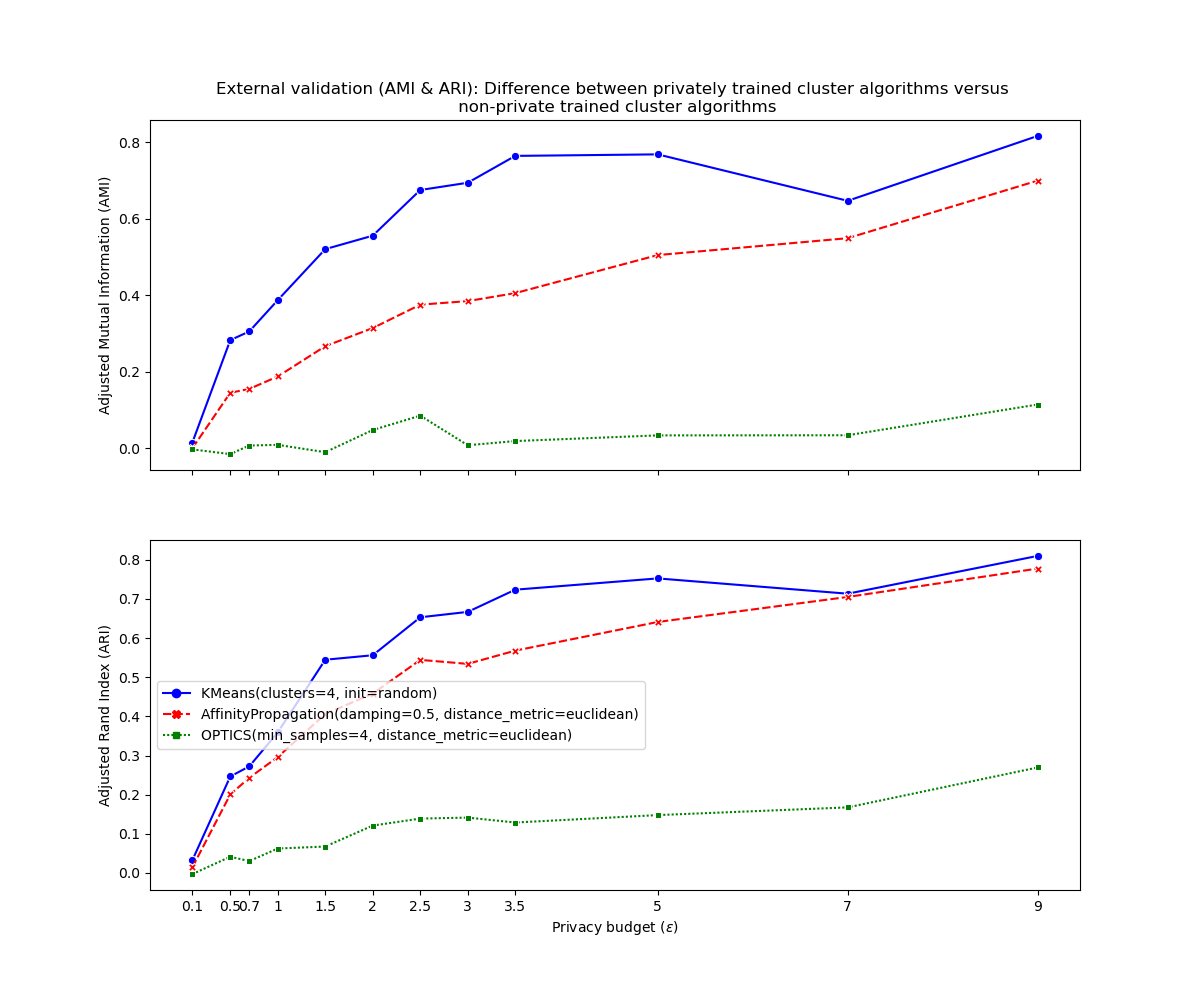
\includegraphics[width=1\textwidth]{Results/2d-laplace-optimal-truncated/seeds-dataset/ami-and-ari.png}
        \caption{External validation (ARI/ AMI) for the 2-dimensional data seeds-dataset for kd-Laplace with optimal truncation}
        \label{fig:external-validation-seeds-dataset_comparison_2d-laplace}
    \end{minipage}
    \begin{minipage}[c]{0.49\textwidth}
        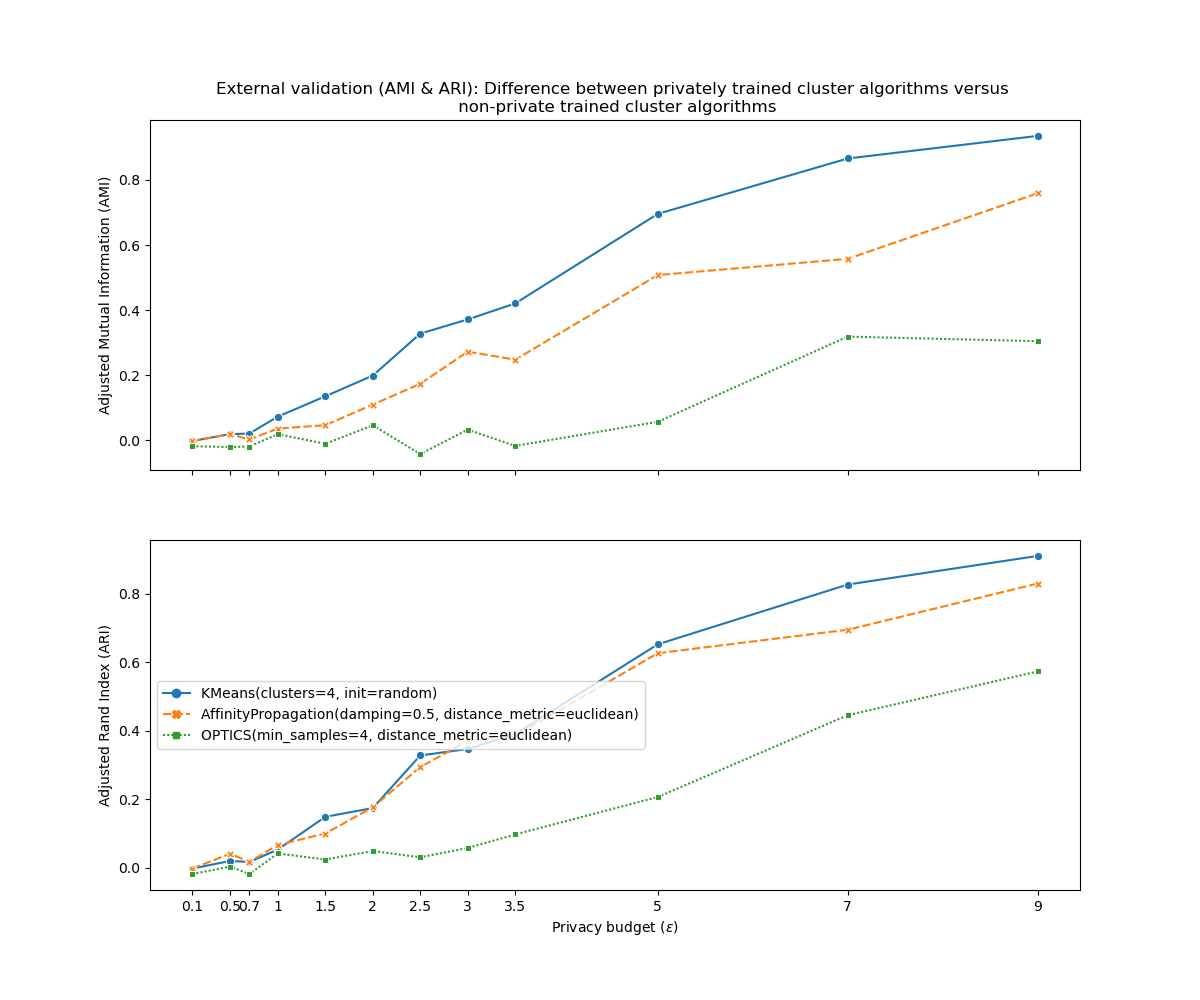
\includegraphics[width=1\textwidth]{Results/2d-piecewise/seeds-dataset/ami-and-ari.png}
        \caption{External validation (ARI/ AMI) for the 2-dimensional data seeds-dataset for piecewise mechanism}
        \label{fig:external-validation-seeds-dataset_comparison_2d-piecewise}
    \end{minipage}

\end{figure}
The above plots show the AMI and ARI scores for the seeds-dataset with kd-laplace/grid/optimal (left-side) and piecewise (right-side).
Piecewise shows a higher AMI / ARI for epsilons 7 and 9. In contrast, the kd-Laplace mechanism scores higher for all the other epsilons (0.1 onward 7).
K-Means achieves the best score for kd-Laplace with a slight margin compared to AP.
However, for the Piecewise mechanism, K-Means performs better.
For both the mechanisms, OPTICS underperforms heavily but still scores the same as AP for Piecewise.
\begin{figure}[H]
    \caption{External validation piecewise \& kd-Laplace/grid/optimal mechanisms for the 2-dimensional data heart-dataset}
    \centering
    \begin{minipage}[c]{0.49\textwidth}
        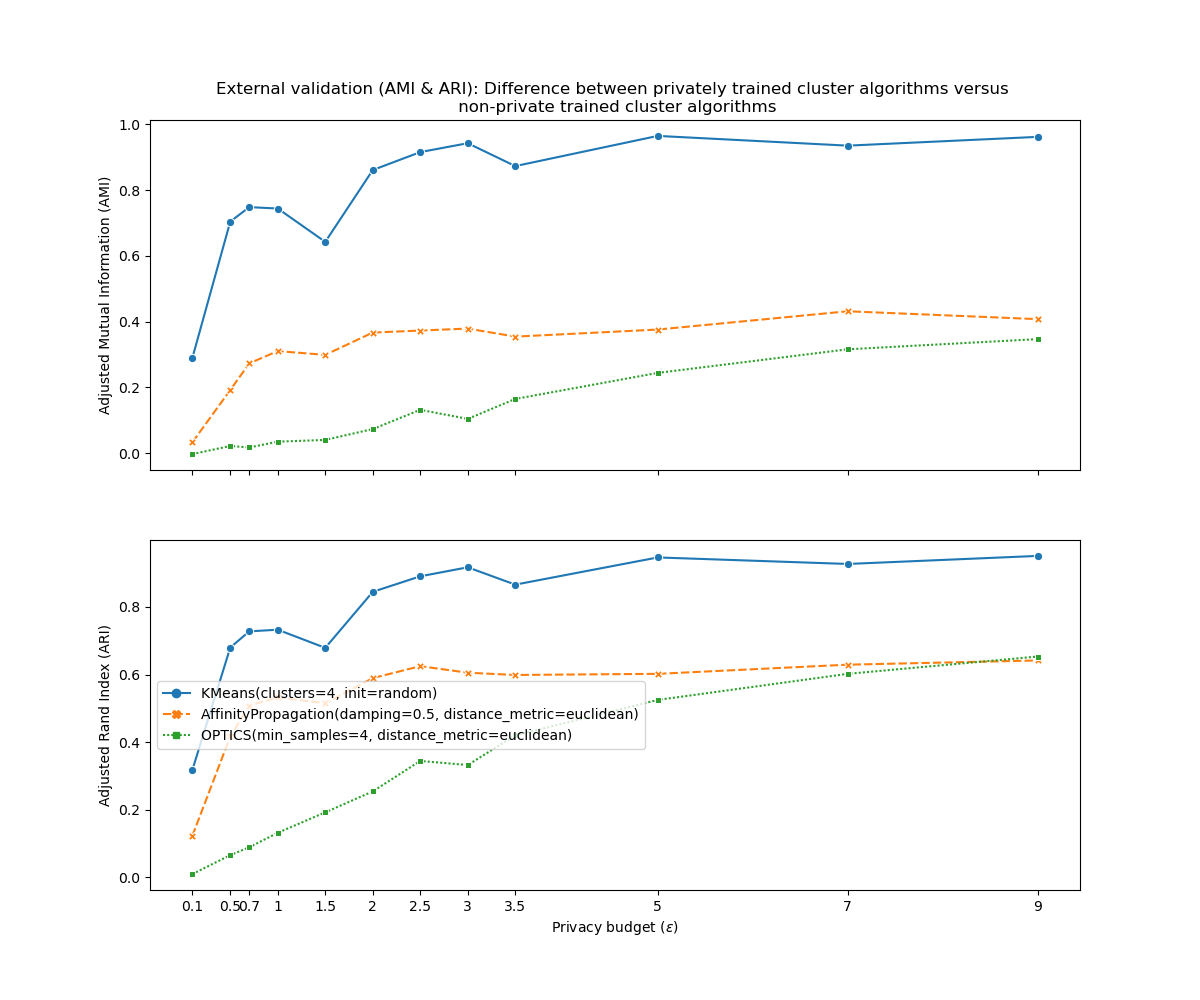
\includegraphics[width=1\textwidth]{Results/2d-laplace-optimal-truncated/heart-dataset/ami-and-ari.png}
        \caption{External validation (ARI/ AMI) for the 2-dimensional data heart-dataset for kd-Laplace with optimal truncation}
        \label{fig:external-validation-heart-dataset_comparison_2d-laplace}
    \end{minipage}
    \begin{minipage}[c]{0.49\textwidth}
        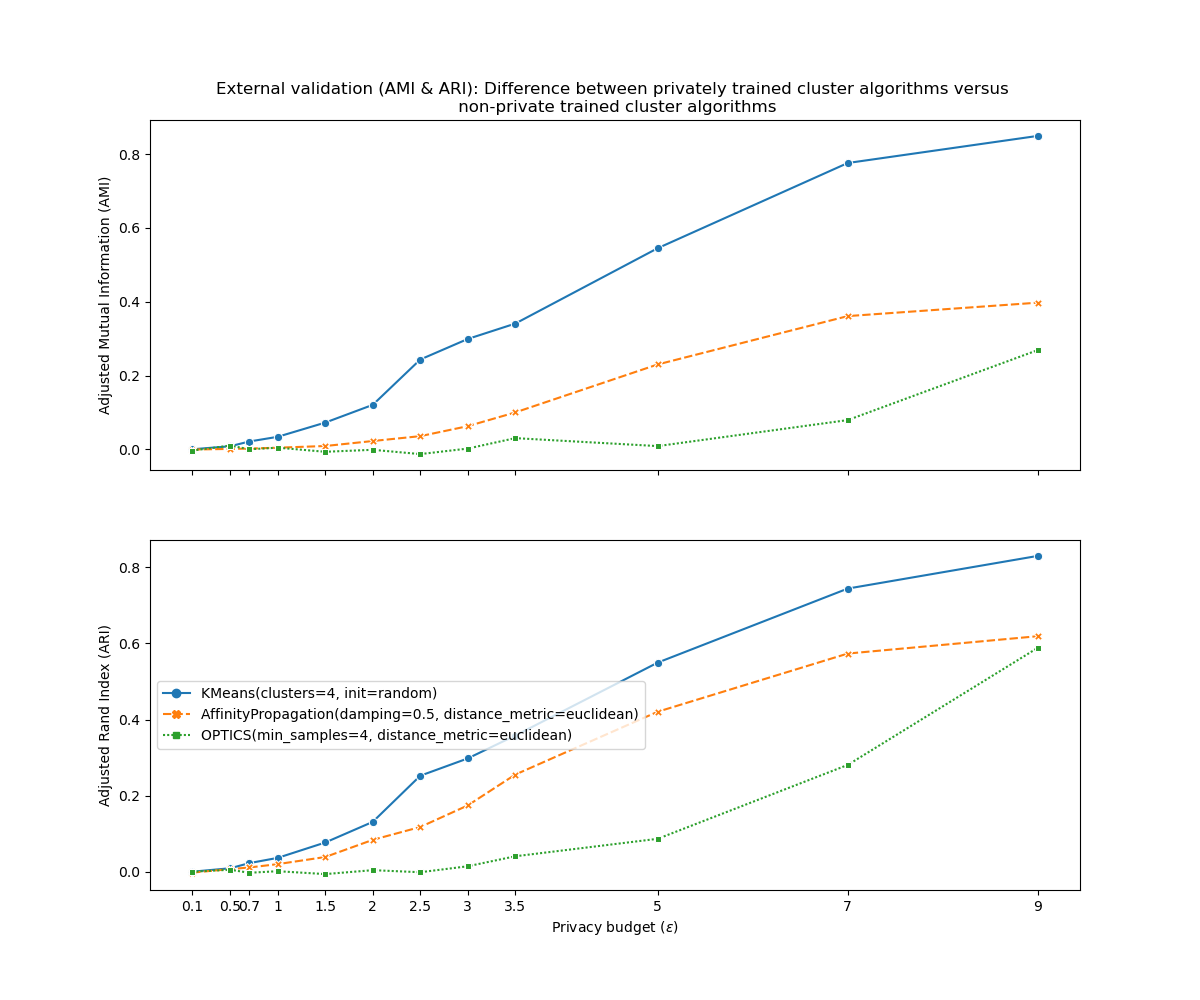
\includegraphics[width=1\textwidth]{Results/2d-piecewise/heart-dataset/ami-and-ari.png}
        \caption{External validation (ARI/ AMI) for the 2-dimensional data heart-dataset for piecewise mechanism}
        \label{fig:external-validation-heart-dataset_comparison_2d-piecewise}
    \end{minipage}
\end{figure}
The kd-Laplace mechanism performs better (0.8 - 1.0 from epsilon 1.0 to 9) for all epsilons for K-Means.
\gls{ap} and OPTICS show the same trend, reaching their peaks around epsilon 7 and 9.
Both underperform by delivering maximum results for these epsilons below 0.3-0.4 AMI/ARI.\newline
\newpage
\subsection{3-dimensional data}
\begin{figure}[H]
    \caption{External validation piecewise \& kd-Laplace/grid/optimal for the 3-dimensional data seeds-dataset}
    \centering
    \begin{minipage}[c]{0.60\textwidth}
        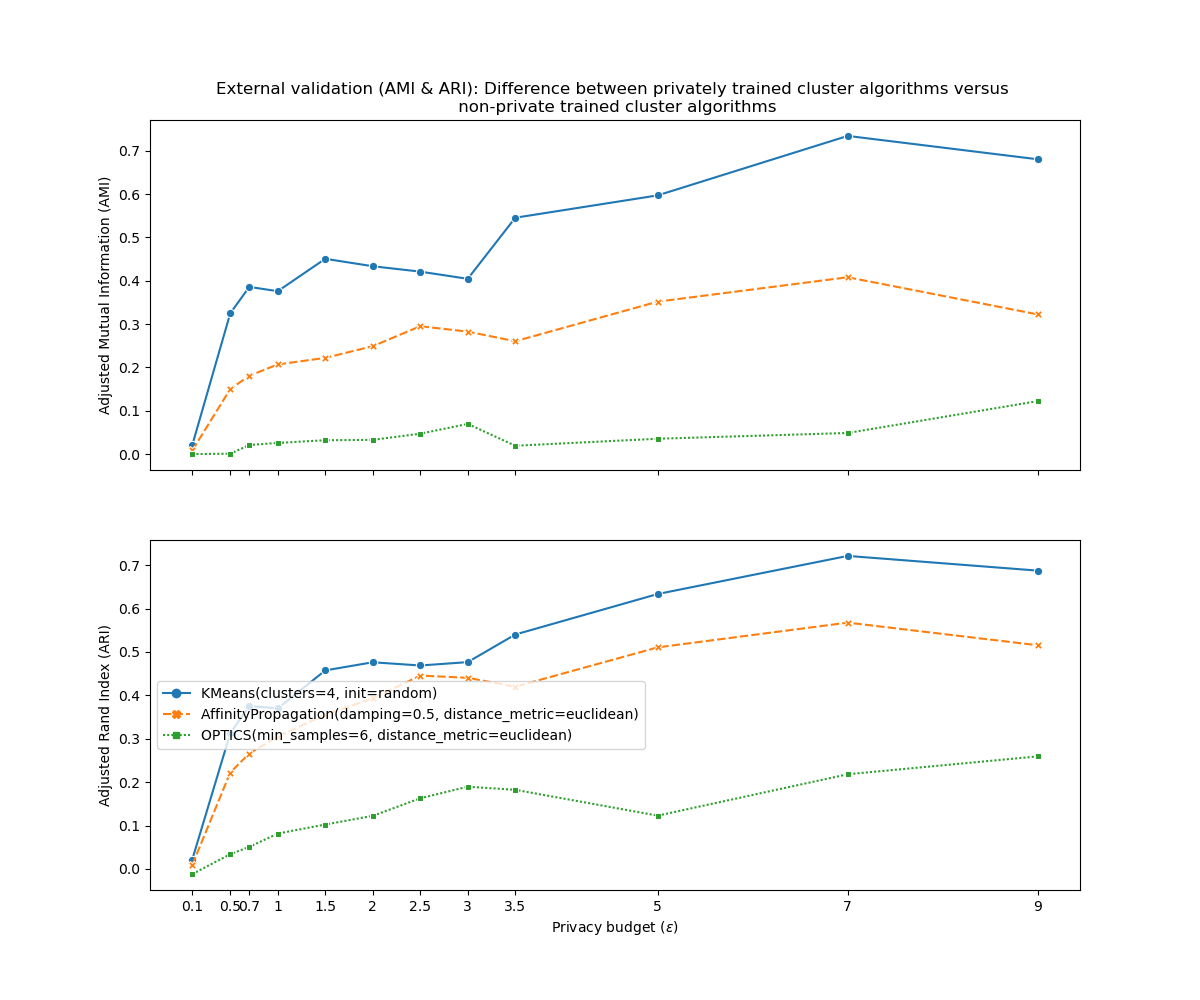
\includegraphics[width=1\textwidth]{Results/3d-laplace-optimal-truncated/seeds-dataset/ami-and-ari.png}
        \caption{External validation (ARI/ AMI) for the 3-dimensional data seeds-dataset for kd-Laplace}
        \label{fig:external-validation-seeds-dataset_comparison_3d-laplace}
    \end{minipage}
    \begin{minipage}[c]{0.60\textwidth}
        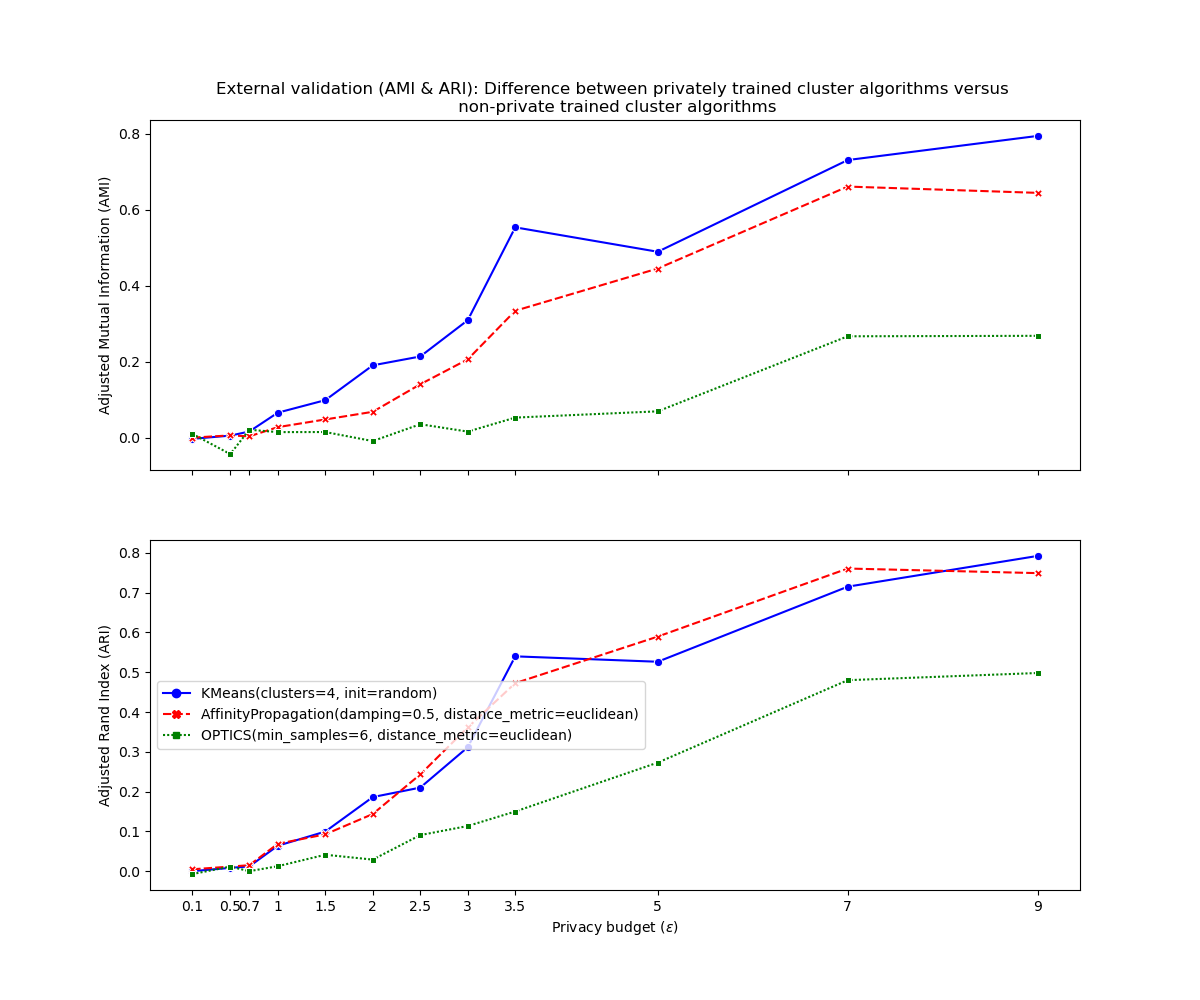
\includegraphics[width=1\textwidth]{Results/3d-piecewise/seeds-dataset/ami-and-ari.png}
        \caption{External validation (ARI/ AMI) for the 3-dimensional data seeds-dataset for piecewise mechanism}
        \label{fig:external-validation-seeds-dataset_comparison_3d-piecewise}
    \end{minipage}
\end{figure}
Piecewise performs better for epsilon 9 but worse for the lower epsilons (0.1 - 5).
K-Means scores 0.7 - 0.8 AMI/ARI, followed by \gls{ap}, which is 0.6.
The kd-Laplace mechanism, on the other hand, shows more difference (K-Means 0.65 - 0.7 and AP 0.3 - 0.2).
OPTICS scores are again low but show a slight upwards trend when the epsilon increases.

\begin{figure}[H]
    \caption{External validation piecewise \& kd-Laplace/grid/optimal mechanisms for the 3-dimensional data heart-dataset}
    \centering
    \begin{minipage}[c]{0.60\textwidth}
        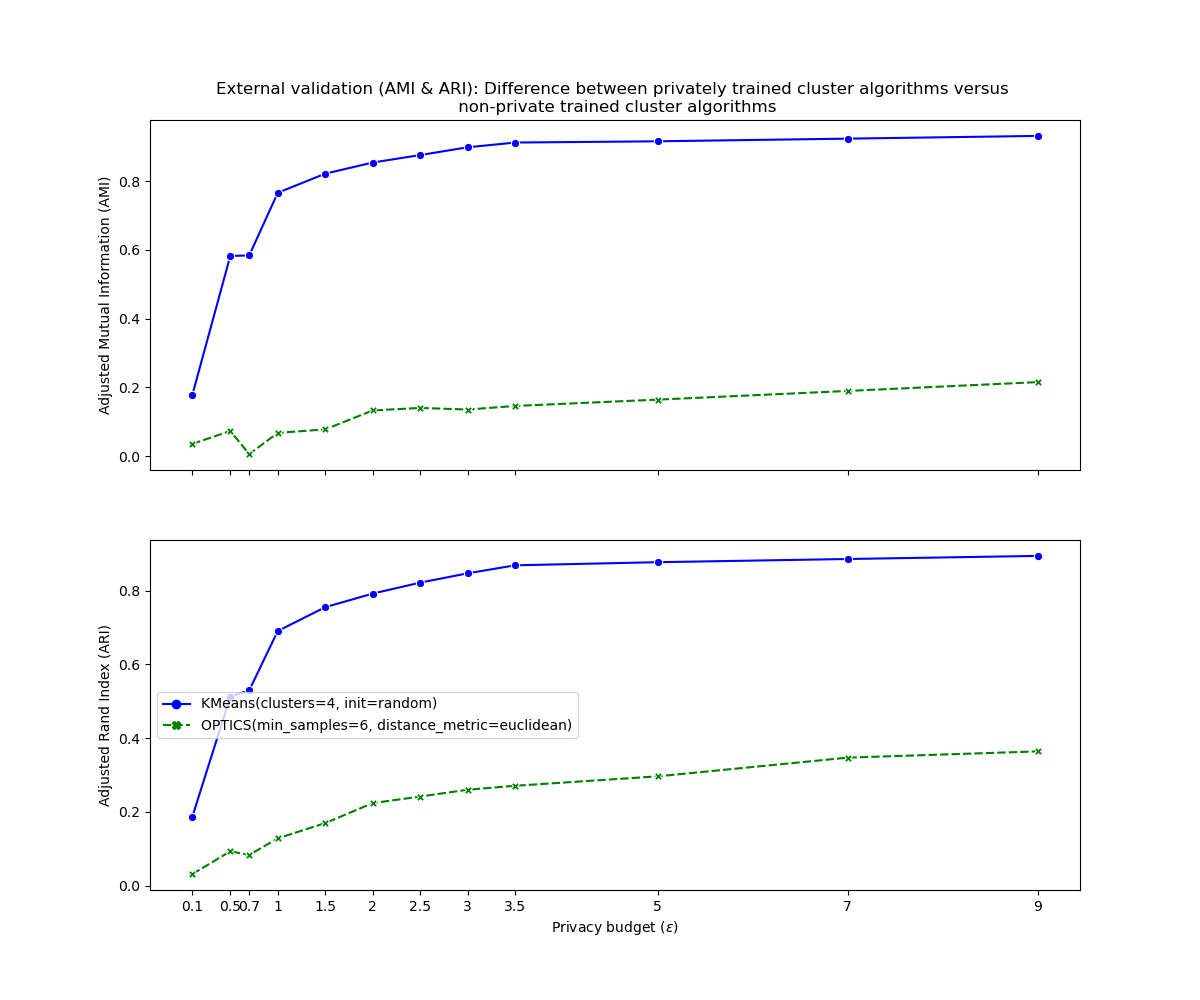
\includegraphics[width=1\textwidth]{Results/3d-laplace-optimal-truncated/heart-dataset/ami-and-ari.png}
        \caption{External validation (ARI/ AMI) for the 3-dimensional data heart-dataset for kd-Laplace with optimal truncation}
        \label{fig:external-validation-heart-dataset_comparison_3d-laplace}
    \end{minipage}
    \begin{minipage}[c]{0.60\textwidth}
        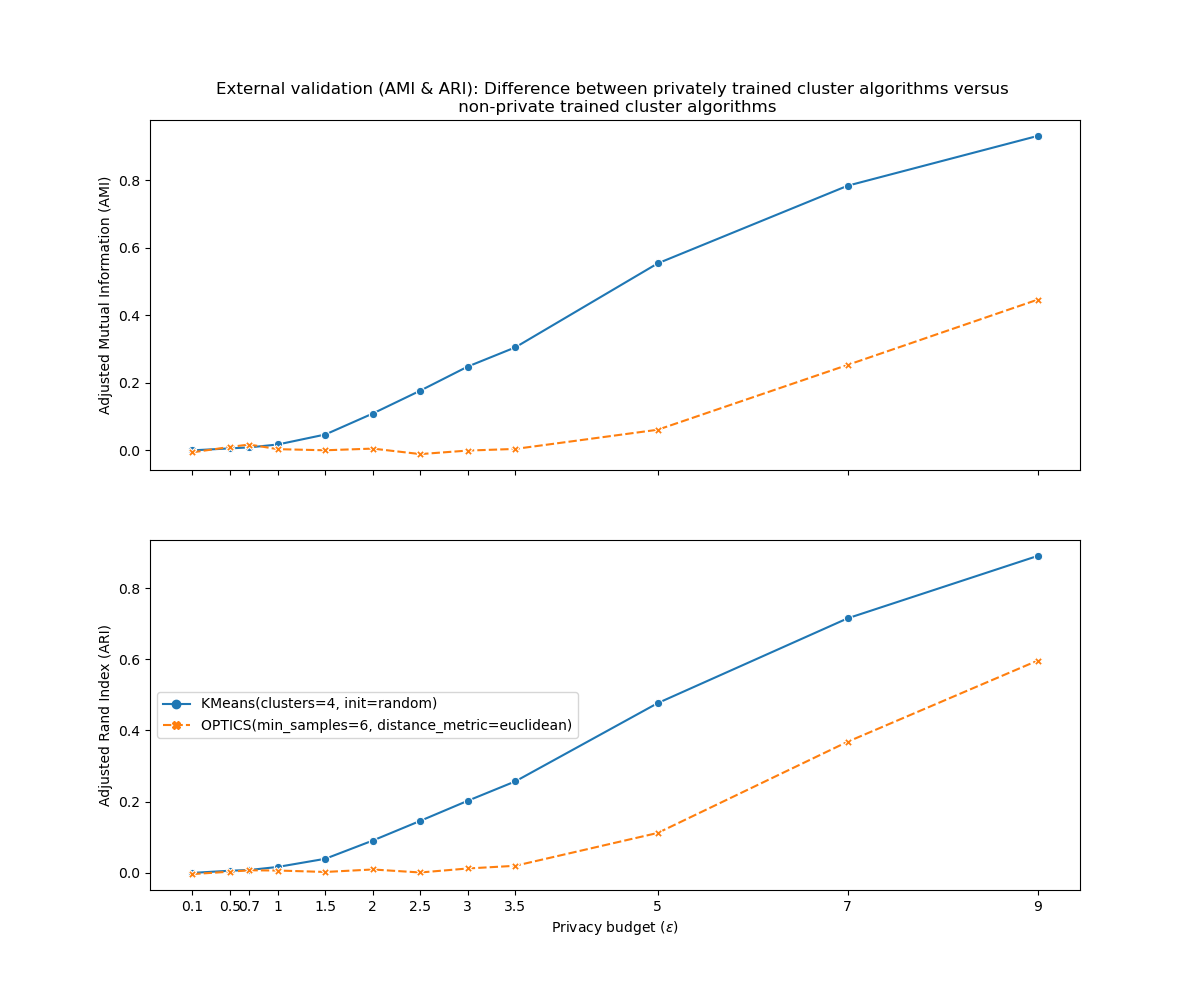
\includegraphics[width=1\textwidth]{Results/3d-piecewise/heart-dataset/ami-and-ari.png}
        \caption{External validation (ARI/ AMI) for the 3-dimensional data heart-dataset for piecewise mechanism}
        \label{fig:external-validation-heart-dataset_comparison_3d-piecewise}
    \end{minipage}
\end{figure}
Piecewise for K-Means performs well (0.78 and 0.93 ARI) for epsilon 7 and 9, respectively.
However, from epsilon 1 onwards kd-Laplace scores 0.77 to 0.93 ARI for K-Means.
On the other hand, OPTICS scores low for kd-Laplace.
It shows an upward trend for Piecewise as the algorithm scores 0.45 ARI and 0.6 AMI for epsilon 9.
While kd-Laplace scores 0.22 ARI and 0.36 AMI for epsilon 9.
OPTICS scores below 0.4 ARI/AMI for both mechanisms if the epsilon is < 9.

\subsection{n-dimensional data}
\begin{figure}[H]
    \caption{External validation piecewise \& kd-Laplace/grid/optimal mechanisms for the n-dimensional data seeds-dataset}
    \centering
    \begin{minipage}[c]{0.60\textwidth}
        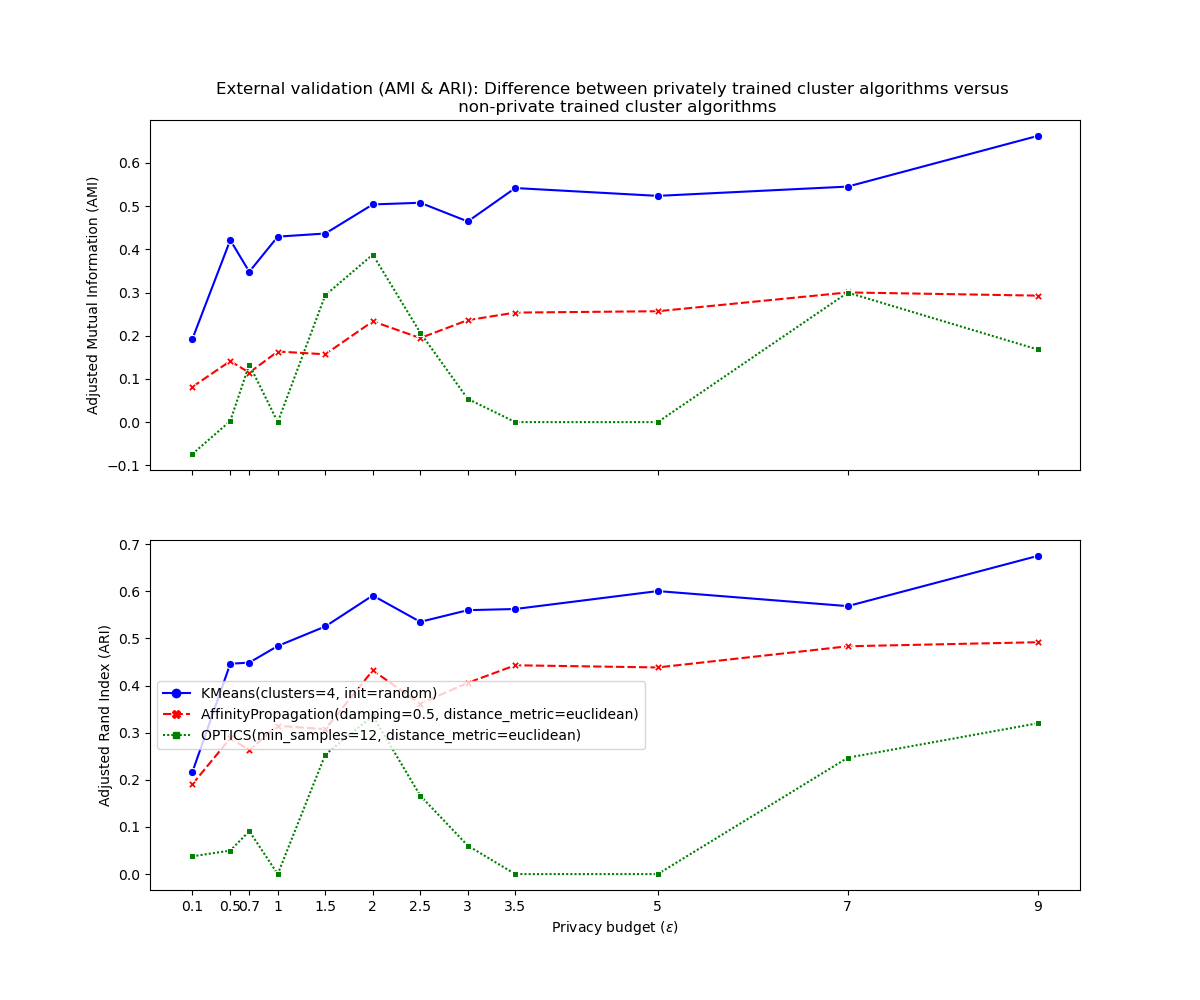
\includegraphics[width=1\textwidth]{Results/nd-laplace-optimal-truncated/seeds-dataset/ami-and-ari.png}
        \caption{External validation (ARI/ AMI) for the n-dimensional data seeds-dataset for kd-Laplace with optimal truncation}
        \label{fig:external-validation-seeds-dataset_comparison_nd-laplace}
    \end{minipage}
    \begin{minipage}[c]{0.60\textwidth}
        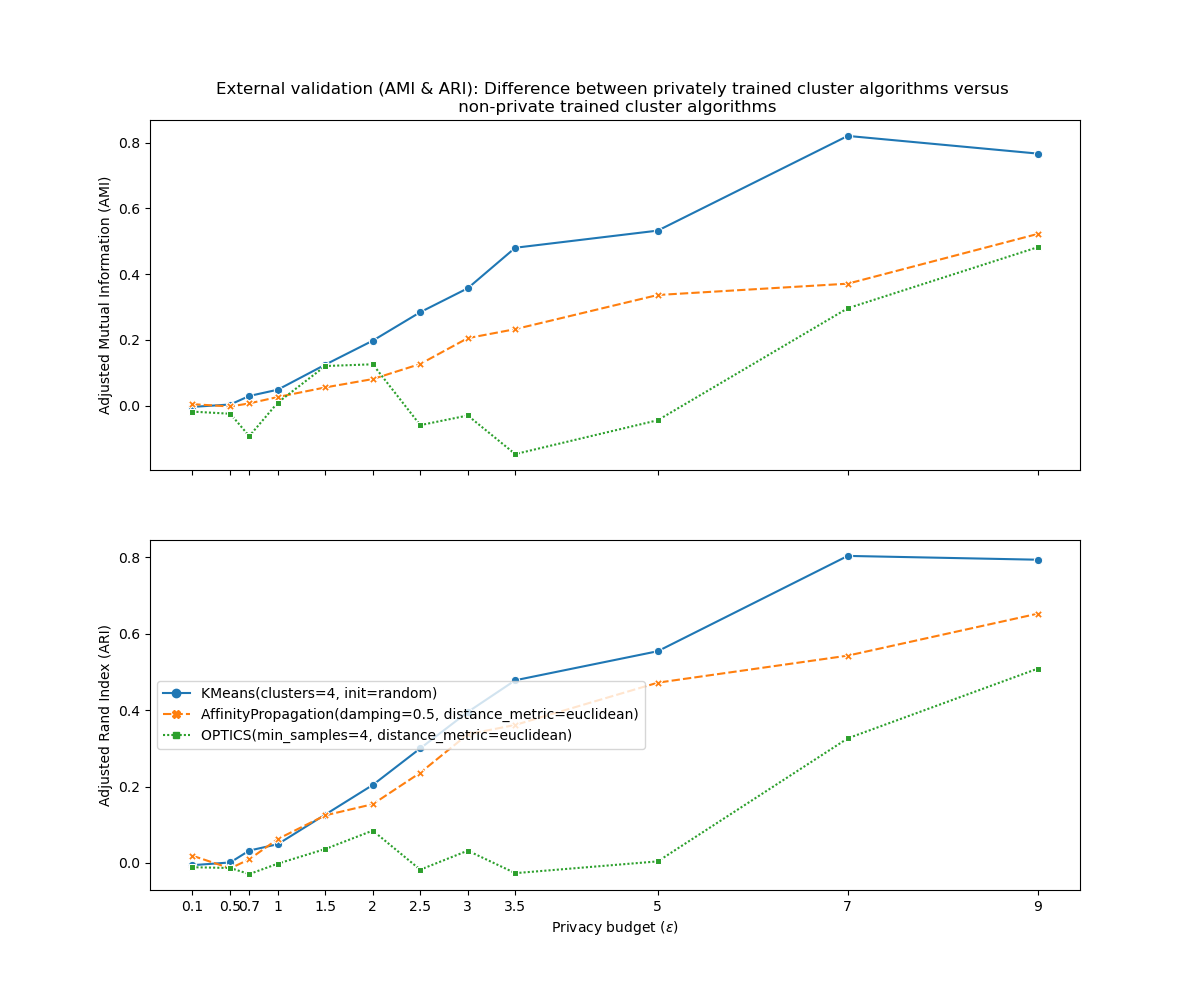
\includegraphics[width=1\textwidth]{Results/nd-piecewise/seeds-dataset/ami-and-ari.png}
        \caption{External validation (ARI/ AMI) for the n-dimensional data seeds-dataset for piecewise mechanism}
        \label{fig:external-validation-seeds-dataset_comparison_nd-piecewise}
    \end{minipage}
\end{figure}
The above plots show the ARI and AMI scores for the heart dataset with kd-laplace/grid/optimal (left-side) and piecewise (right-side).
Piecewise performs well (0.89 and 0.87 ARI) for epsilon 9 and 7 for K-Means, respectively.
In comparison, kd-Laplace scores worse for the same epsilon values (0.56 and 0.51 ARI); on the other hand, kd-Laplace scores better for all the other epsilons.
After K-Means, the best scoring cluster algorithm is OPTICS for Piecewise, with a score of 0.62 ARI for 9 epsilon.
However, the other epsilons \gls{ap} scores better. For kd-Laplace, \gls{ap} is second after K-Means, and OPTICS scores much worse for AMI.
But, for ARI, the scores for OPTICS and \gls{ap} lay close together for epsilon 9.
\begin{figure}[H]
    \caption{External validation piecewise \& kd-Laplace/grid/optimal mechanisms for the n-dimensional data heart-dataset}
    \centering
    \begin{minipage}[c]{0.60\textwidth}
        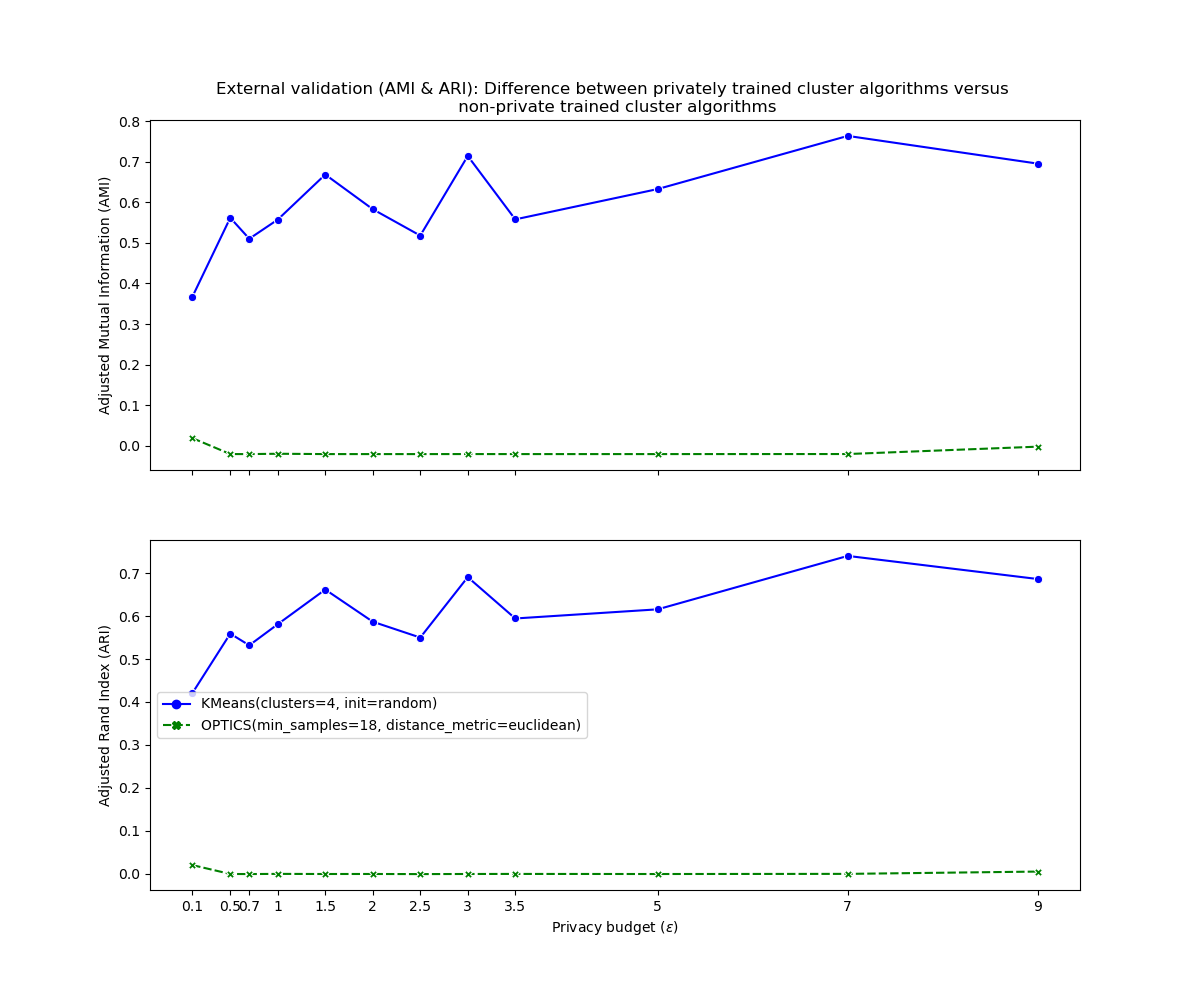
\includegraphics[width=1\textwidth]{Results/nd-laplace-optimal-truncated/heart-dataset/ami-and-ari.png}
        \caption{External validation (ARI/ AMI) for the n-dimensional data heart-dataset for kd-Laplace with optimal truncation}
        \label{fig:external-validation-heart-dataset_comparison_nd-laplace}
    \end{minipage}
    \begin{minipage}[c]{0.60\textwidth}
        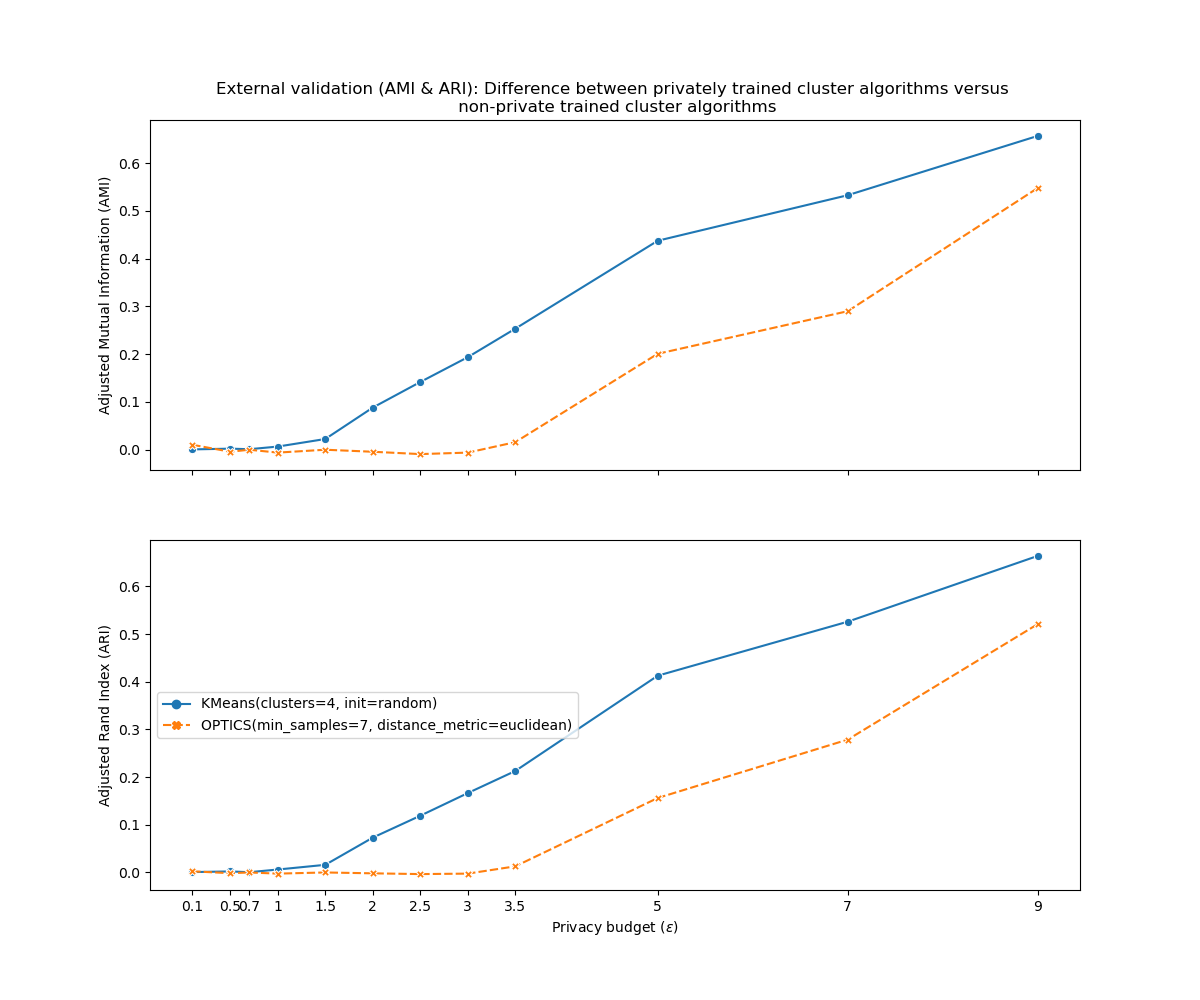
\includegraphics[width=1\textwidth]{Results/nd-piecewise/heart-dataset/ami-and-ari.png}
        \caption{External validation (ARI/ AMI) for the n-dimensional data heart-dataset for piecewise mechanism}
        \label{fig:external-validation-heart-dataset_comparison_nd-piecewise}
    \end{minipage}
\end{figure}
Piecewise shows similar trends for K-Means and OPICS. But, K-Means scores better (0.65 ARI) for epsilon 9, while OPTICS peaks at 0.5 ARI.
However, Piecewise scores (<0.2 ARI) for epsilon 0.1 til 3.5.
In contrast, kd-Laplace scores more evenly (0.6 - 0.7 ARI) between epsilon 3.5 and 9. Conversely, OPTICS scores lower (< 0.2 ARI) for all epsilon values.
\section{Mechanism utility}
In the sections below, the different types of Laplace mechanisms and piecewise are compared using a barplot.
Since ARI and AMI provide the same information, we show only the Adjusted Mutual Information (AMI) to avoid redundant information.
For the same reason, only the K-Means algorithm was used to calculate the AMI.
The x-axis displays the privacy budget, and the y-axis shows the corresponding AMI.
The privacy mechanisms are displayed as follows:
\begin{enumerate}
    \item \textbf{Piecewise:} Displayed as a yellow bar or line.
    \item \textbf{kd-Laplace:} Displayed as a red bar or line.
    \item \textbf{kd-Laplace/grid:} Displayed as a blue bar or line.
    \item \textbf{kd-Laplace/grid/optimal:} Displayed as a green bar or line.
\end{enumerate}

Please refer to the plots in the appendix for internal validation: \ref{appendix:results-cluster-utility}.
\newpage
\subsection{2-dimensional data}
\begin{figure}[H]
    \centering
    \begin{minipage}[c]{0.8\textwidth}
        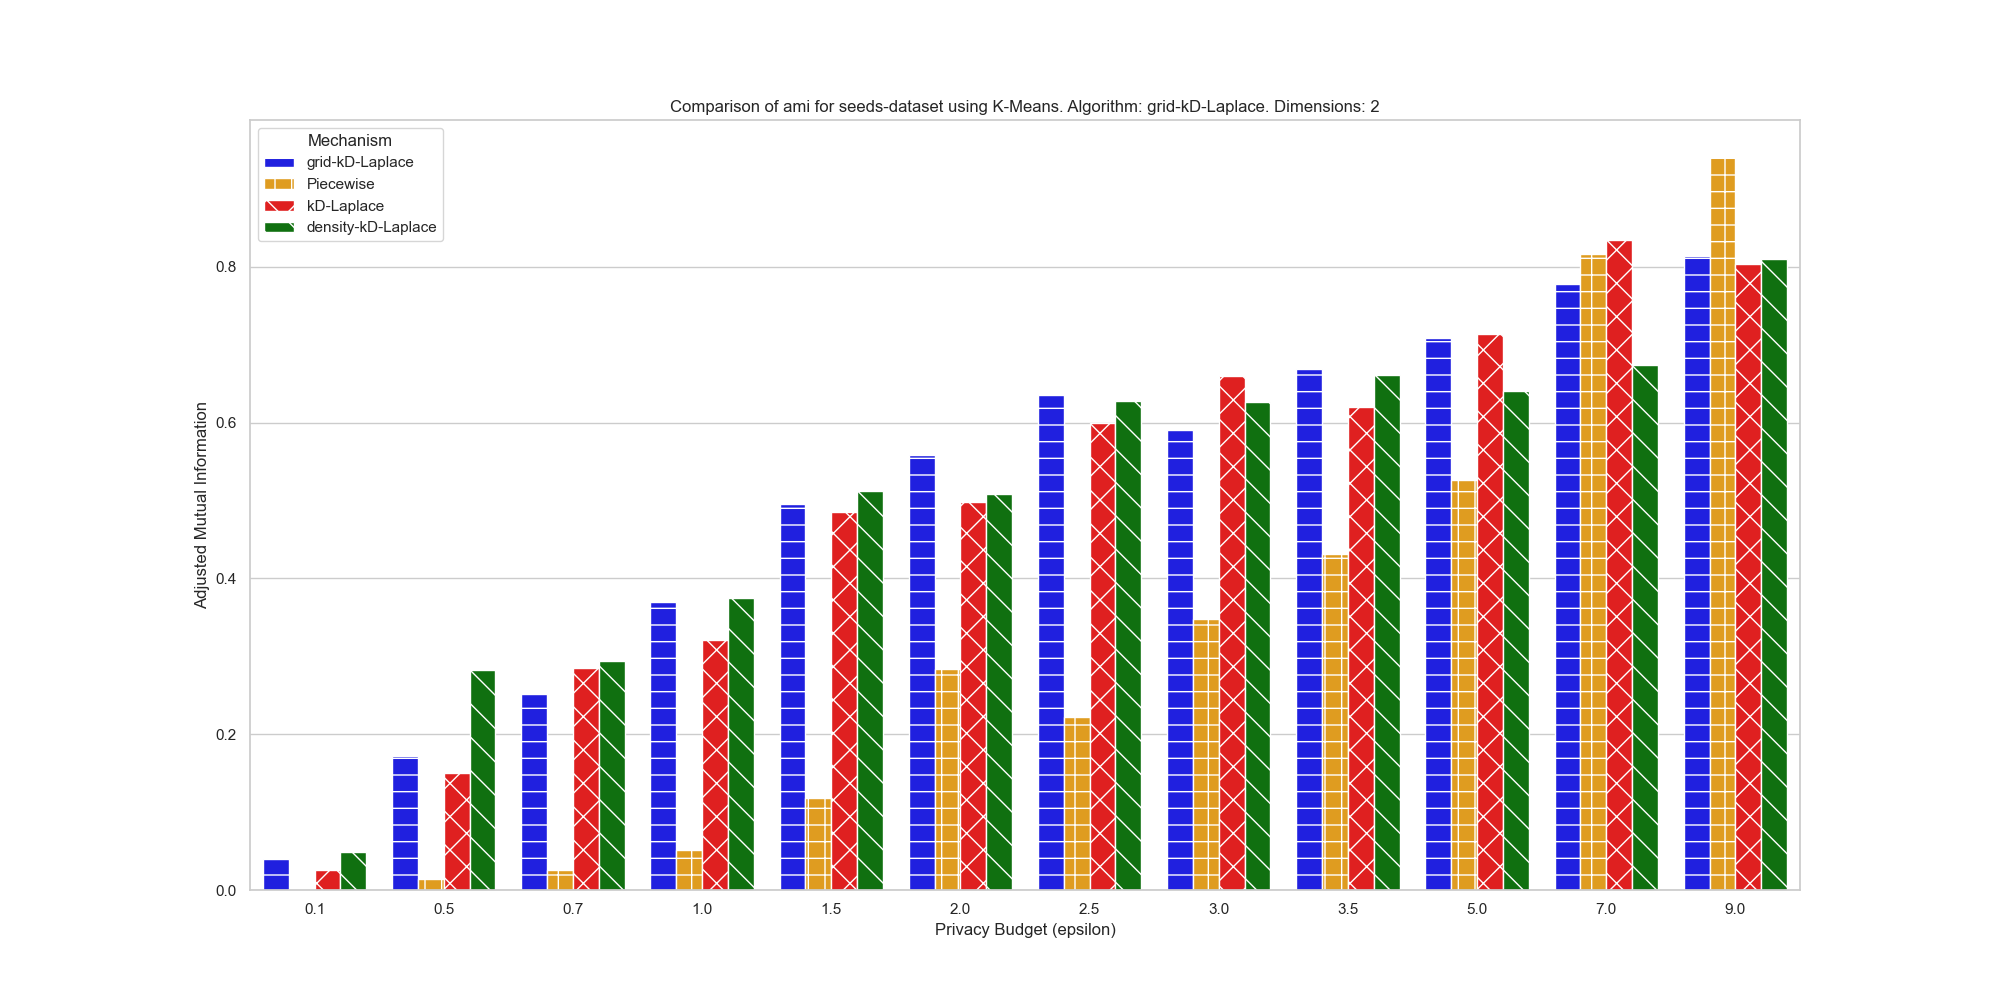
\includegraphics[width=1\textwidth]{Results/RQ1/seeds-dataset/ami_seeds-dataset_comparison.png}
        \caption{Adjusted Mutual Information comparison for the seeds-dataset}
        \label{fig:ami_seeds-dataset_comparison_2d}
    \end{minipage}
    \begin{minipage}[c]{0.8\textwidth}
        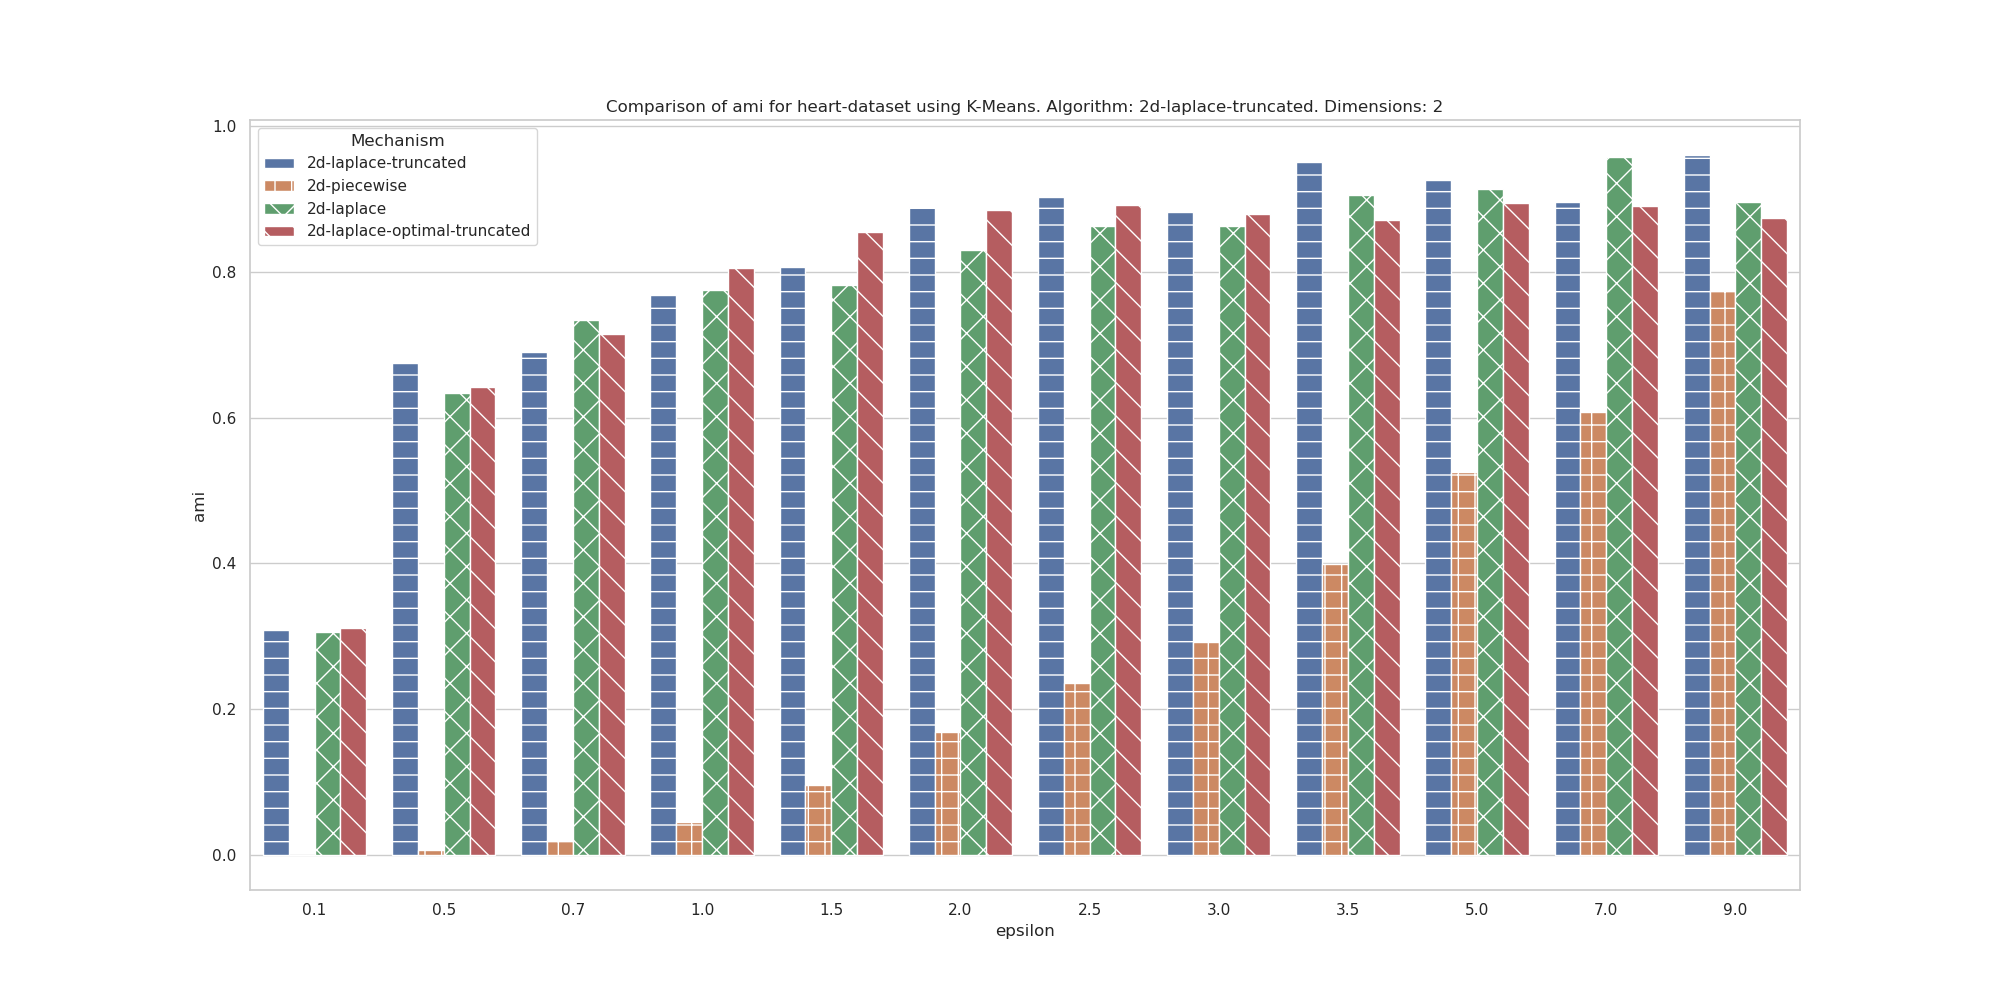
\includegraphics[width=1\textwidth]{Results/RQ1/heart-dataset/ami_heart-dataset_comparison.png}
        \caption{Adjusted Mutual Information comparison for the heart-dataset}
        \label{fig:ami_heart-dataset_comparison_2d}
    \end{minipage}

\end{figure}
The two plots compare external validation (AMI) between the two privacy frameworks, Piecewise, and kd-Laplace, with three variants.
A clear trend in AMI can be observed in the top plot, with the lowest epsilon (0.1) yielding the lowest score for the mechanisms.
Piecewise consistently scores lower for all epsilons, except for epsilons 7 and 9.
Additionally, we notice minimal differences among the variants of kd-Laplace, but kd-Laplace/grid/optimal performs slightly better for epsilon 0.1 while scoring worse for 7 and 9.
\newpage
\subsection{3-dimensional data}
\begin{figure}[H]
    \centering
    \begin{minipage}[c]{0.8\textwidth}
        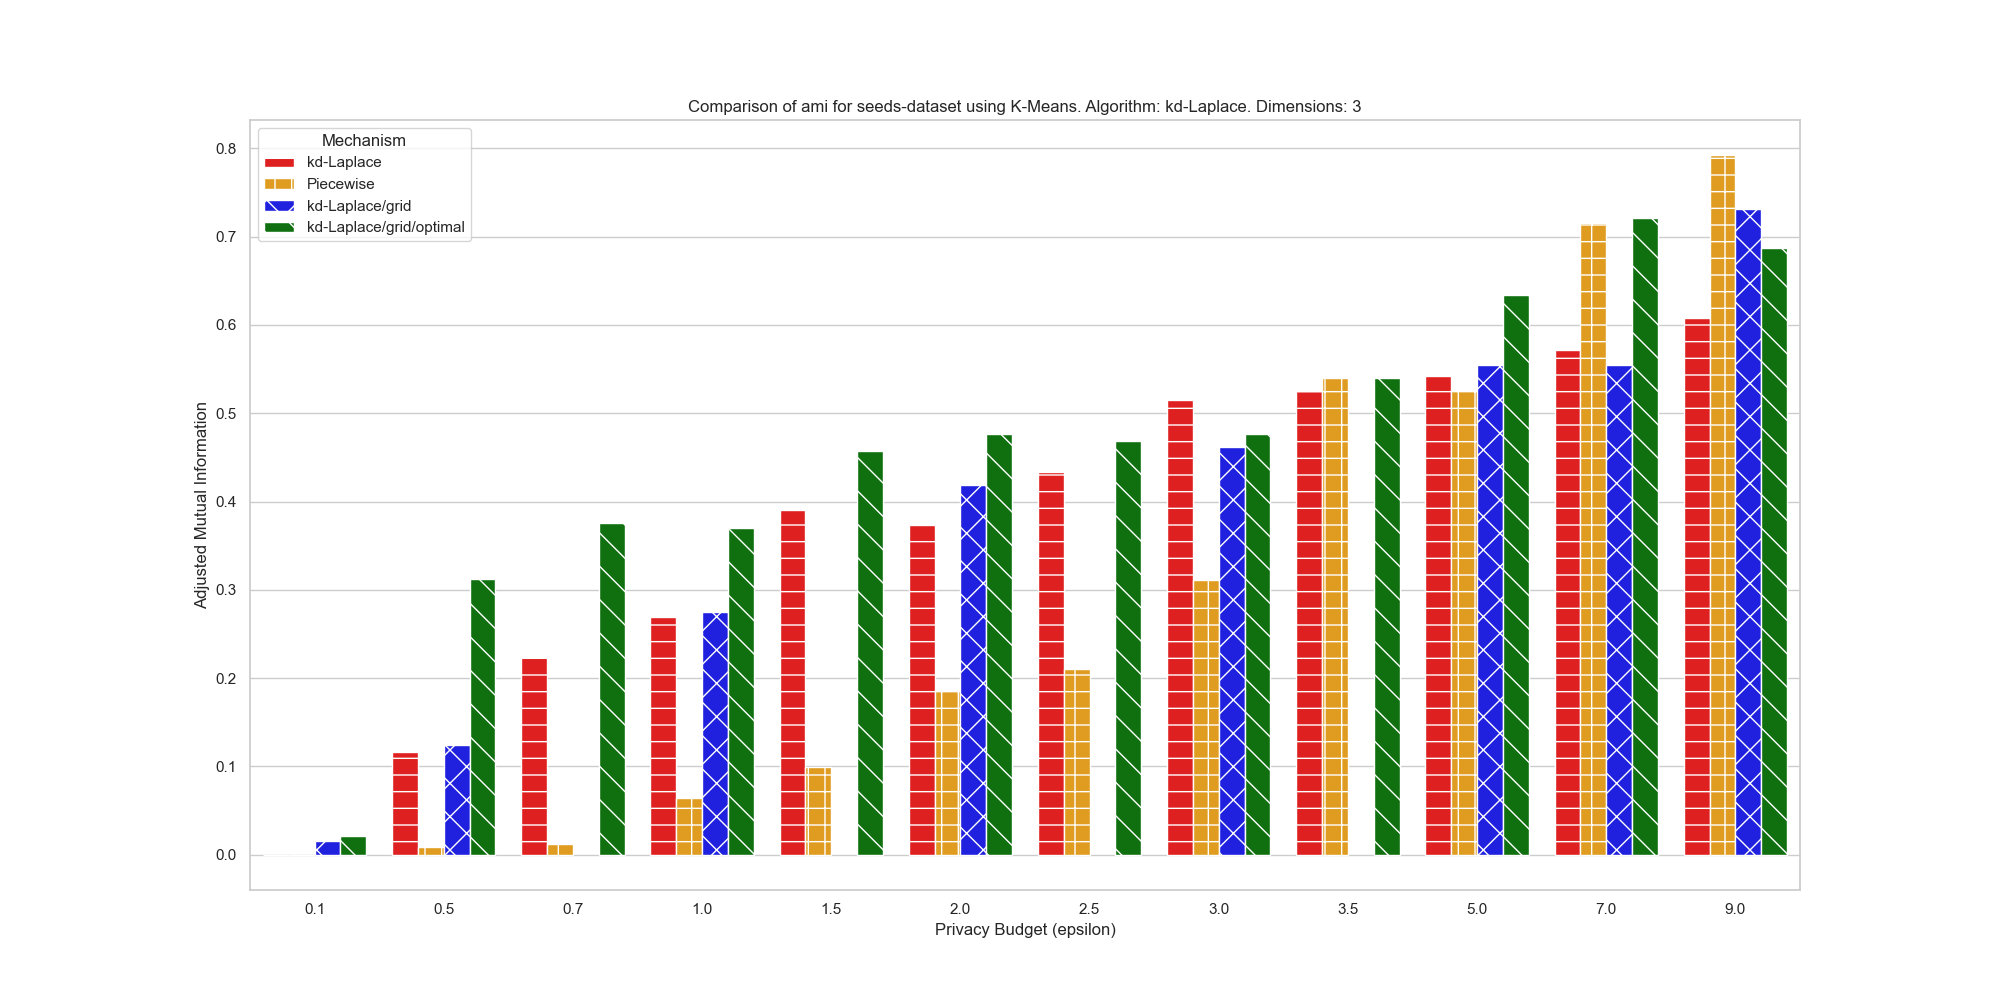
\includegraphics[width=1\textwidth]{Results/RQ2/seeds-dataset/ami_seeds-dataset_comparison.png}
        \caption{Adjusted Mutual Information comparison for the 3-dimensional seeds-dataset}
        \label{fig:ami_seeds-dataset_comparison_3d}
    \end{minipage}
    \begin{minipage}[c]{0.8\textwidth}
        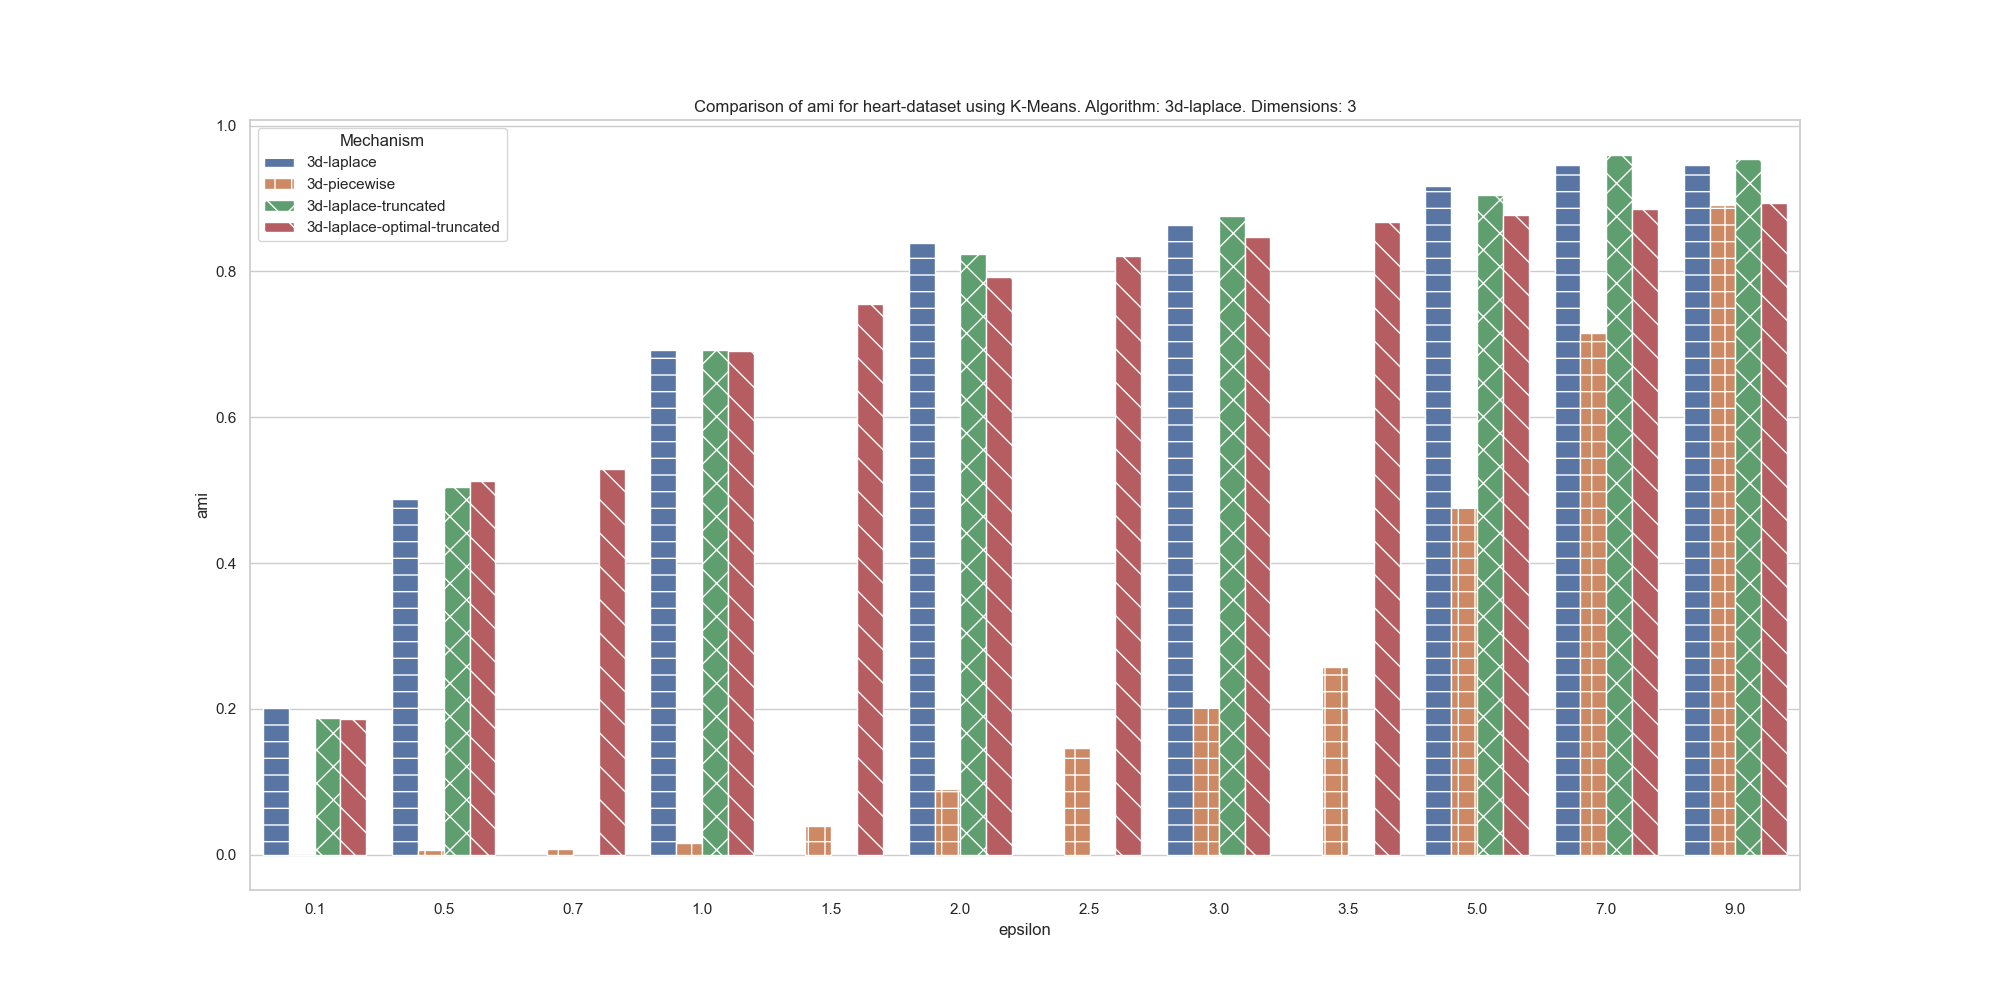
\includegraphics[width=1\textwidth]{Results/RQ2/heart-dataset/ami_heart-dataset_comparison.png}
        \caption{Adjusted Mutual Information comparison for the 3-dimensional heart-dataset}
        \label{fig:ami_heart-dataset_comparison_3d}
    \end{minipage}

\end{figure}
Between the seeds and heart datasets, the kd-Laplace mechanism with variants scored better overall than the piecewise mechanism.
The Piecewise mechanism scores low (< 0.5 ARI) for the epsilons 0.1 to 3.5 in the seeds dataset.
In contrast, kd-Laplace with variants reach this score for around epsilon 3.0.
For epsilon 7 and 9, the Piecewise mechanism catches up with kd-Laplace and scores around equal (0.7 \& 0.8 AMI).
Kd-Laplace/grid/optimal scores are a little better for epsilon 5 and 7, but the difference between the variants is minimal overall.

The kd-Laplace mechanism with variants score > 0.6 AMI for epsilon 1 and higher.
As with the seeds dataset, the Piecewise mechanism scores low (< 0.5 ARI) for the epsilons 0.1 to 7.0.
For epsilon 9, the Piecewise mechanism scores around 0.8 AMI, which equals kd-Laplace.
Between the different kd-Laplace variants, the difference is small. But, kd-Laplace/grid/optimal scores are slightly worse for all epsilons.

\newpage
\subsection{n-dimensional data}
\begin{figure}[H]
    \centering
    \begin{minipage}[c]{0.8\textwidth}
        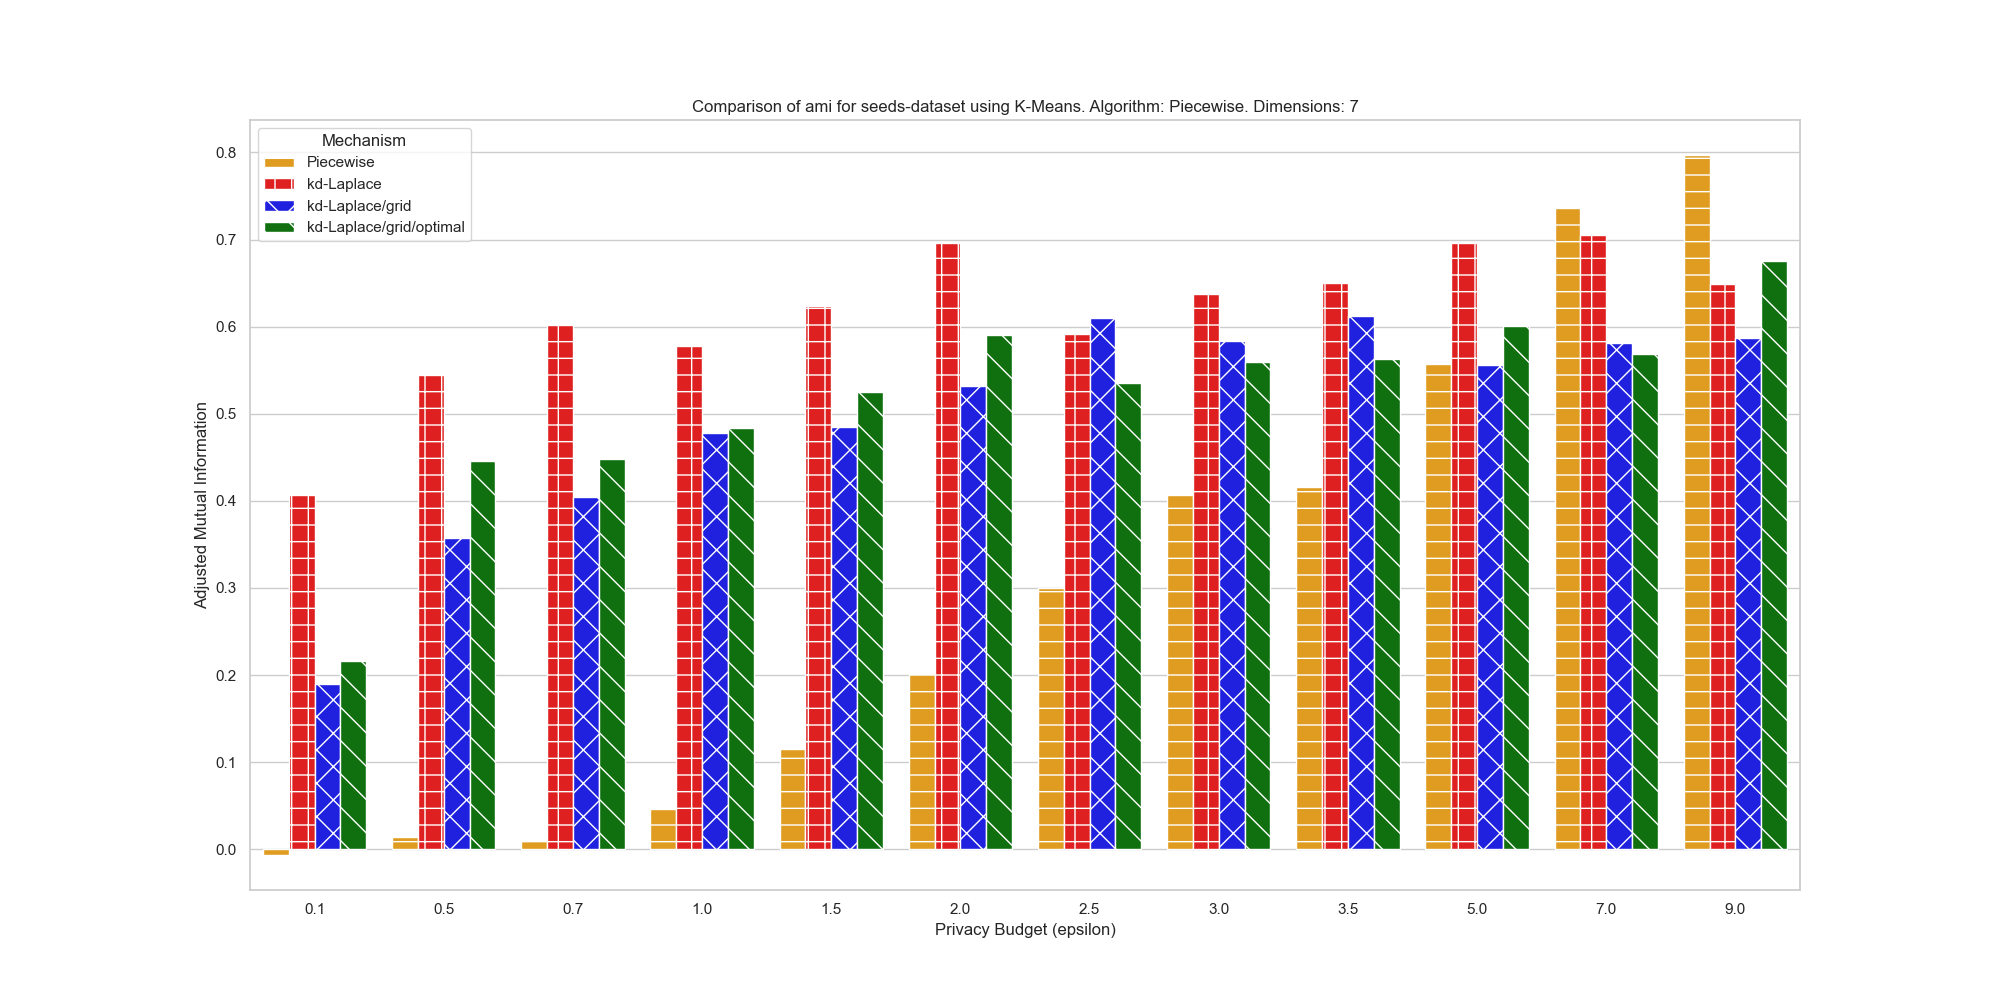
\includegraphics[width=1\textwidth]{Results/RQ2-nd/seeds-dataset/ami_seeds-dataset_comparison.png}
        \caption{Adjusted Mutual Information comparison for all numerical features for the seeds-dataset}
        \label{fig:ami_seeds-dataset_comparison_nd}
    \end{minipage}
    \begin{minipage}[c]{0.8\textwidth}
        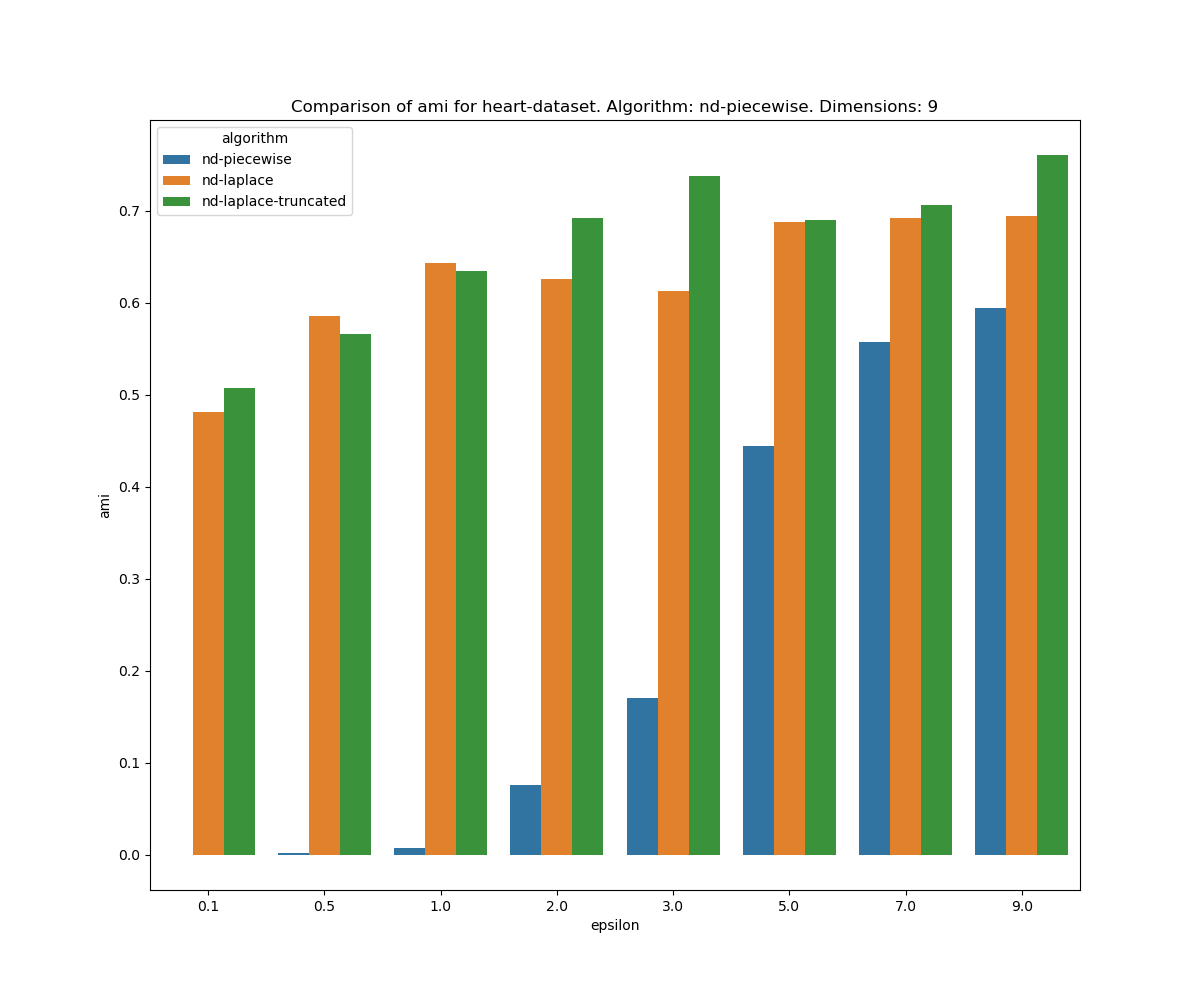
\includegraphics[width=1\textwidth]{Results/RQ2-nd/heart-dataset/ami_heart-dataset_comparison.png}
        \caption{Adjusted Mutual Information comparison for all numerical features for the heart-dataset}
        \label{fig:ami_heart-dataset_comparison_nd}
    \end{minipage}
\end{figure}
The above plot represents the Adjusted Mutual Information (AMI) for n-dimensional data. The seeds dataset (top) shows a clear peak for kd-Laplace without any optimization. Piecewise consistently scores lower than the kd-Laplace variants for most epsilon values, except for epsilon 7 and 9 where Piecewise performs better (AMI > 0.7). The latter performs slightly better among kd-Laplace/grid and kd-Laplace/grid/optimal variants.

For the heart dataset (bottom graph), the scores are relatively similar across all kd-Laplace variants. Piecewise scores below 0.5 AMI until epsilon 7 and performs at an equivalent level as the kd-Laplace variants for epsilon 9. The kd-Laplace variants score significantly better, as they already surpass 0.5 AMI from epsilon 0.5. Among the kd-Laplace variants, kd-Laplace without optimization stands slightly higher (AMI > 0.7).

\newpage
\section{Privacy}
The images below display bar plots for the membership advantage and TPR of membership inference attacks as described in the methodology.
We use the same color scheme in the previous section to display the different mechanisms.
In addition, a red line was drawn to indicate the baseline TPR (the non-private dataset's TPR). \newline
\subsection{2-dimensional data}
\mycomment{\begin{figure}[H]
        \centering
        \begin{minipage}[c]{0.49\textwidth}
            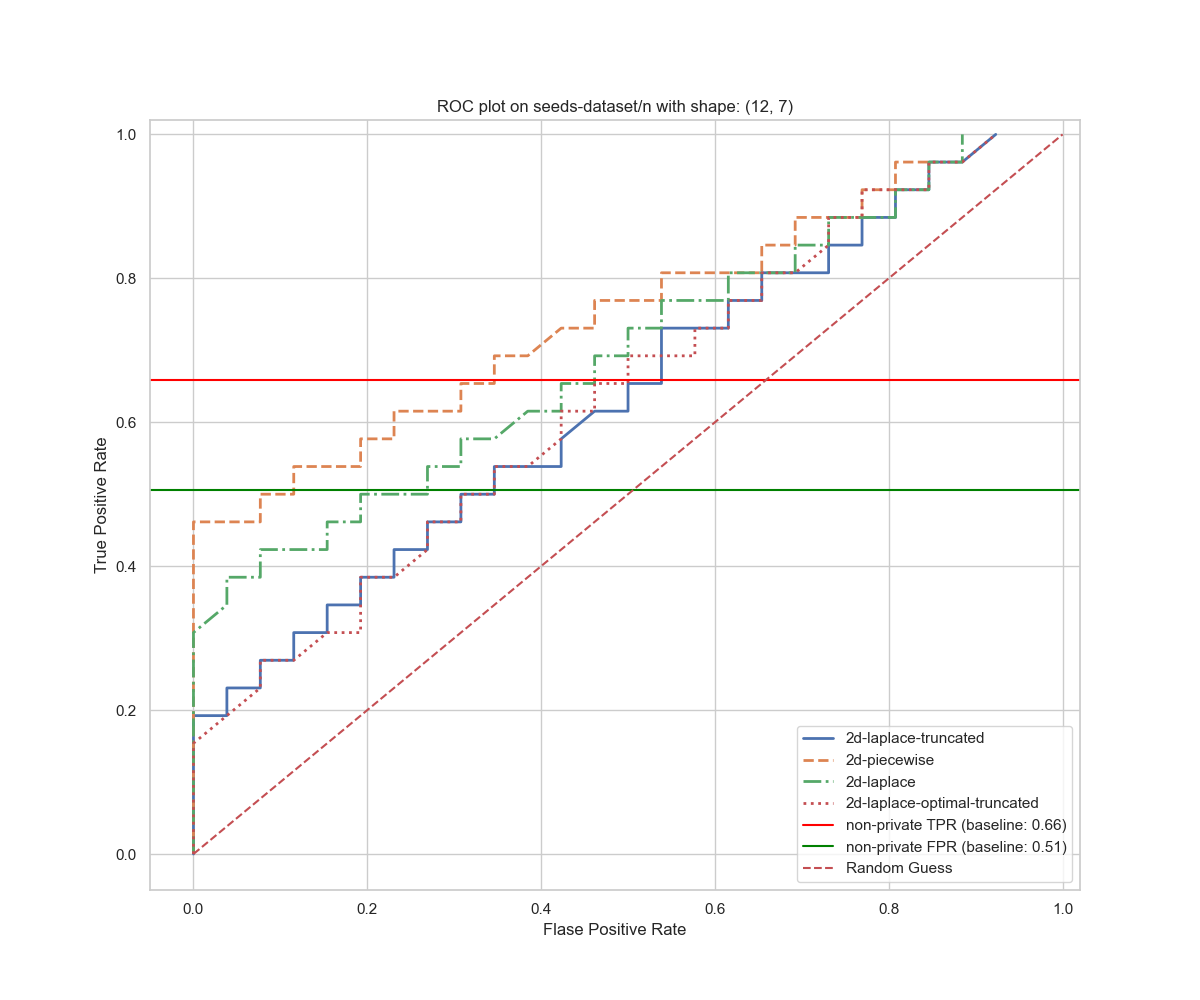
\includegraphics[width=1\textwidth]{Results/RQ1/seeds-dataset/roc_plot.png}
            \caption{ROC-curve for privacy per privacy mechanism for seeds-dataset.}
            \label{fig:privacy_seeds-dataset_comparison_2d_roc_plot}
        \end{minipage}
        \begin{minipage}[c]{0.49\textwidth}
            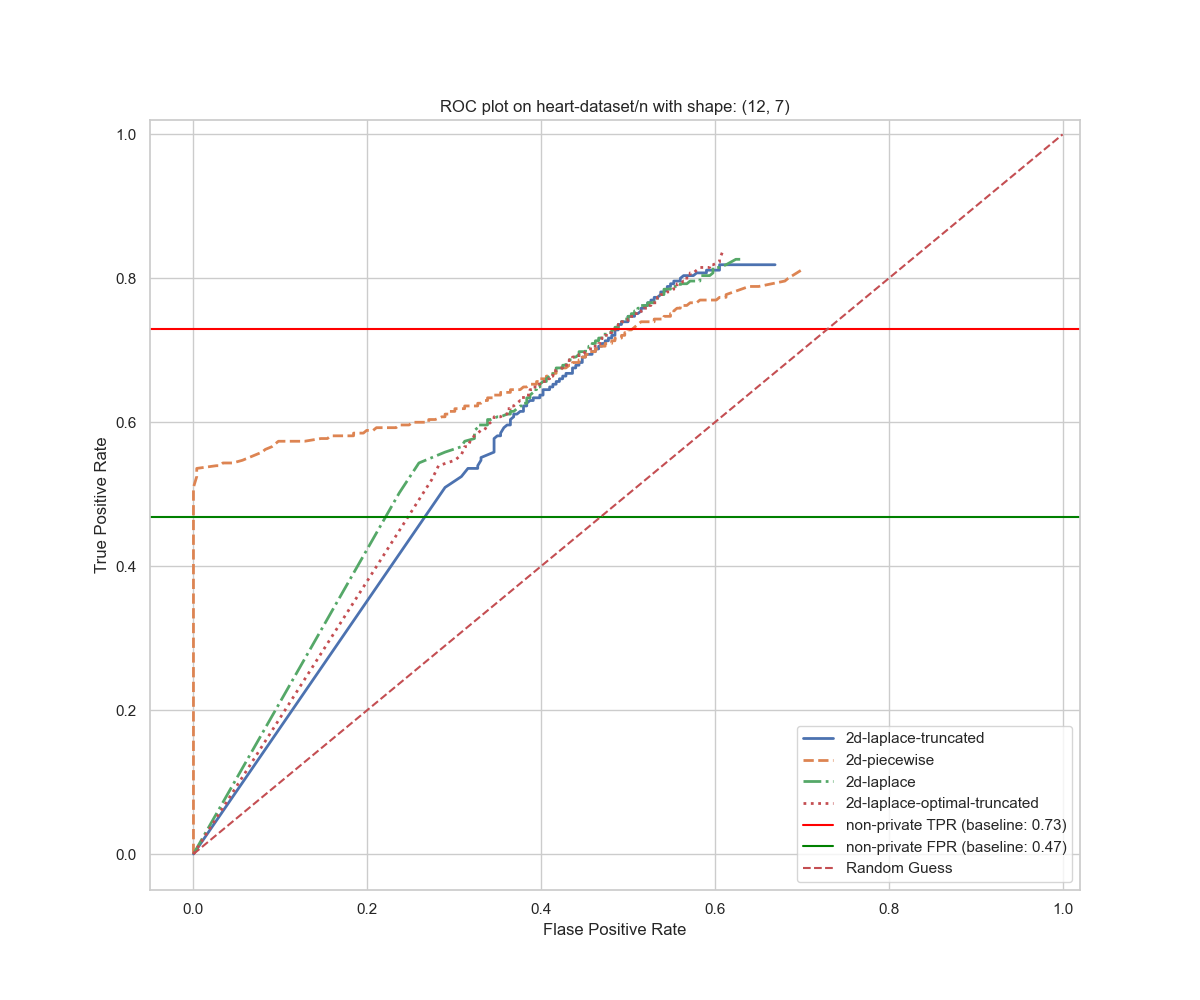
\includegraphics[width=1\textwidth]{Results/RQ1/heart-dataset/roc_plot.png}
            \caption{ROC-curve for privacy per privacy mechanism for heart-dataset.}
            \label{fig:privacy_heart-dataset_comparison_2d_roc_plot}
        \end{minipage}
    \end{figure}}
\begin{figure}[H]
    \centering
    \begin{minipage}[c]{1.1\textwidth}
        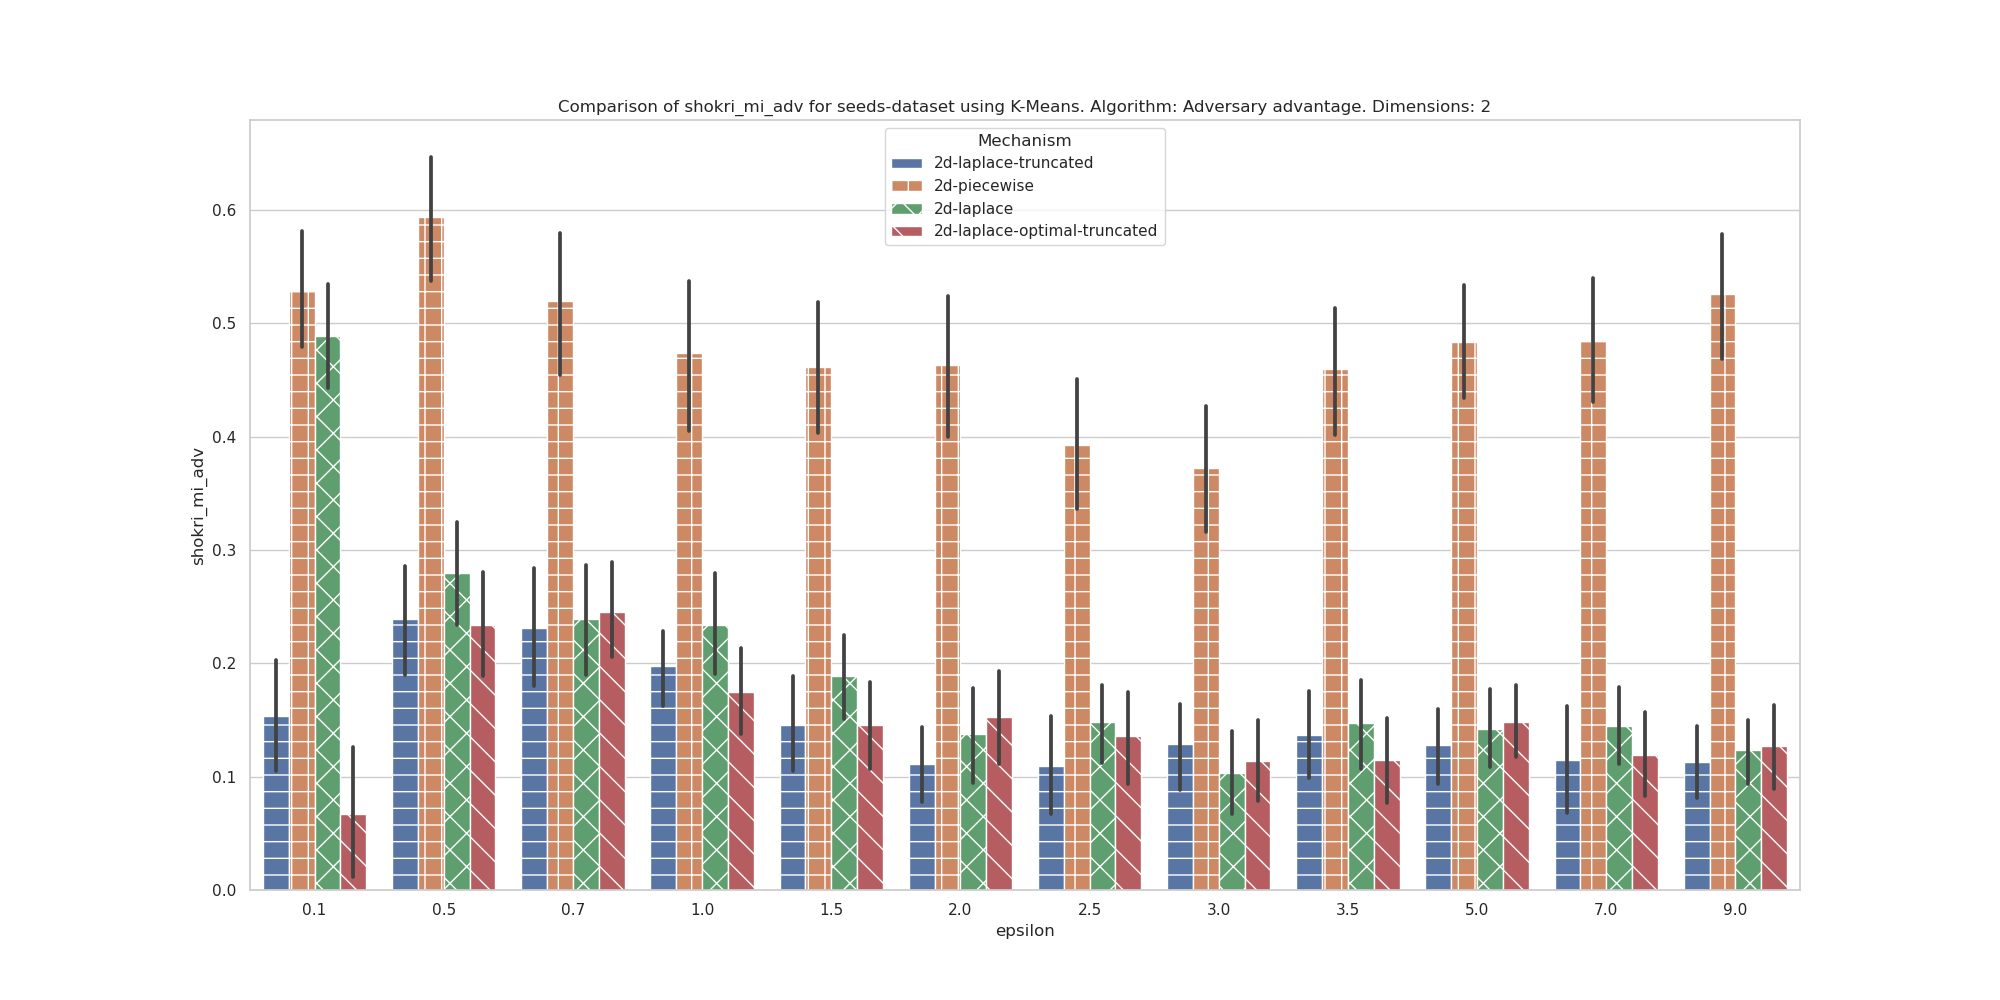
\includegraphics[width=0.50\textwidth]{Results/RQ1/seeds-dataset/shokri_mi_adv_seeds-dataset_comparison.png}
        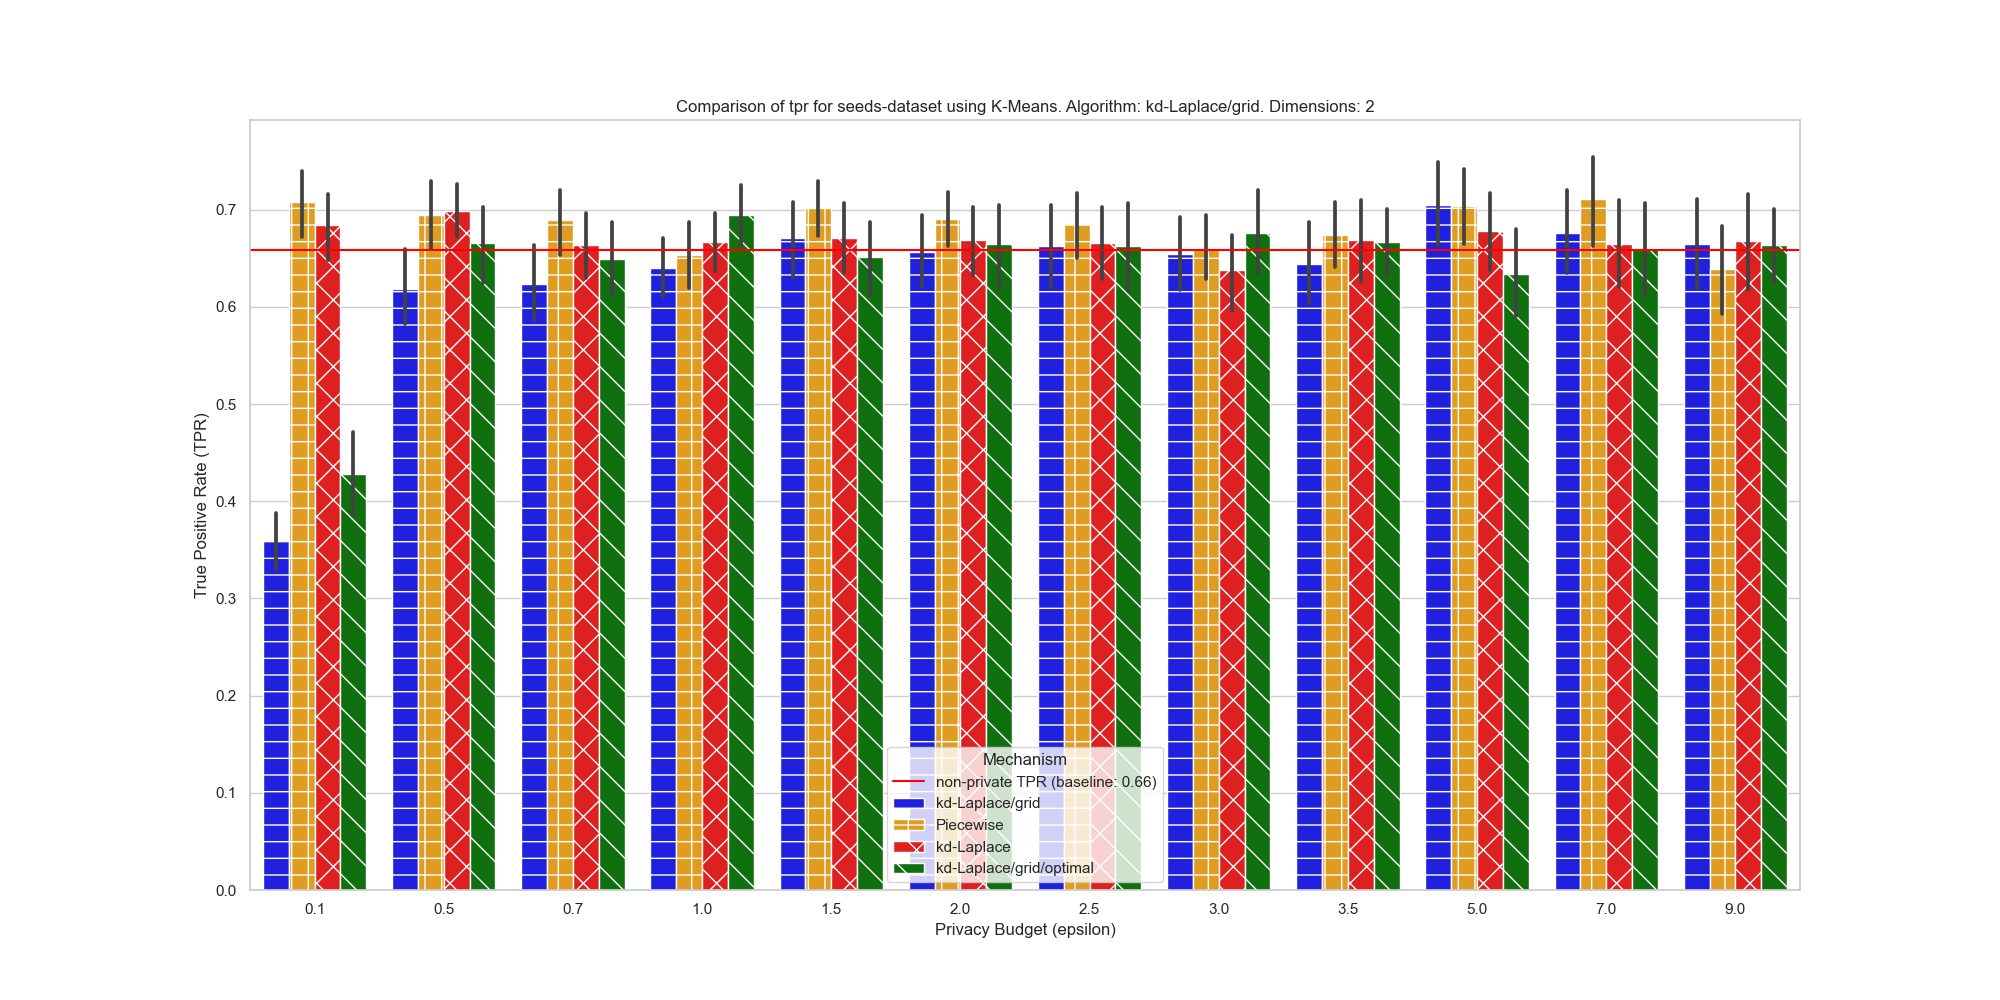
\includegraphics[width=0.50\textwidth]{Results/RQ1/seeds-dataset/tpr_seeds-dataset_comparison.png}
        \caption{Barplot for adversary advantage (left) and TPR (right) per privacy mechanism for seeds-dataset.}
        \label{fig:privacy_seeds-dataset_comparison_2d_aa_plot}
    \end{minipage}
    \begin{minipage}[c]{1.1\textwidth}
        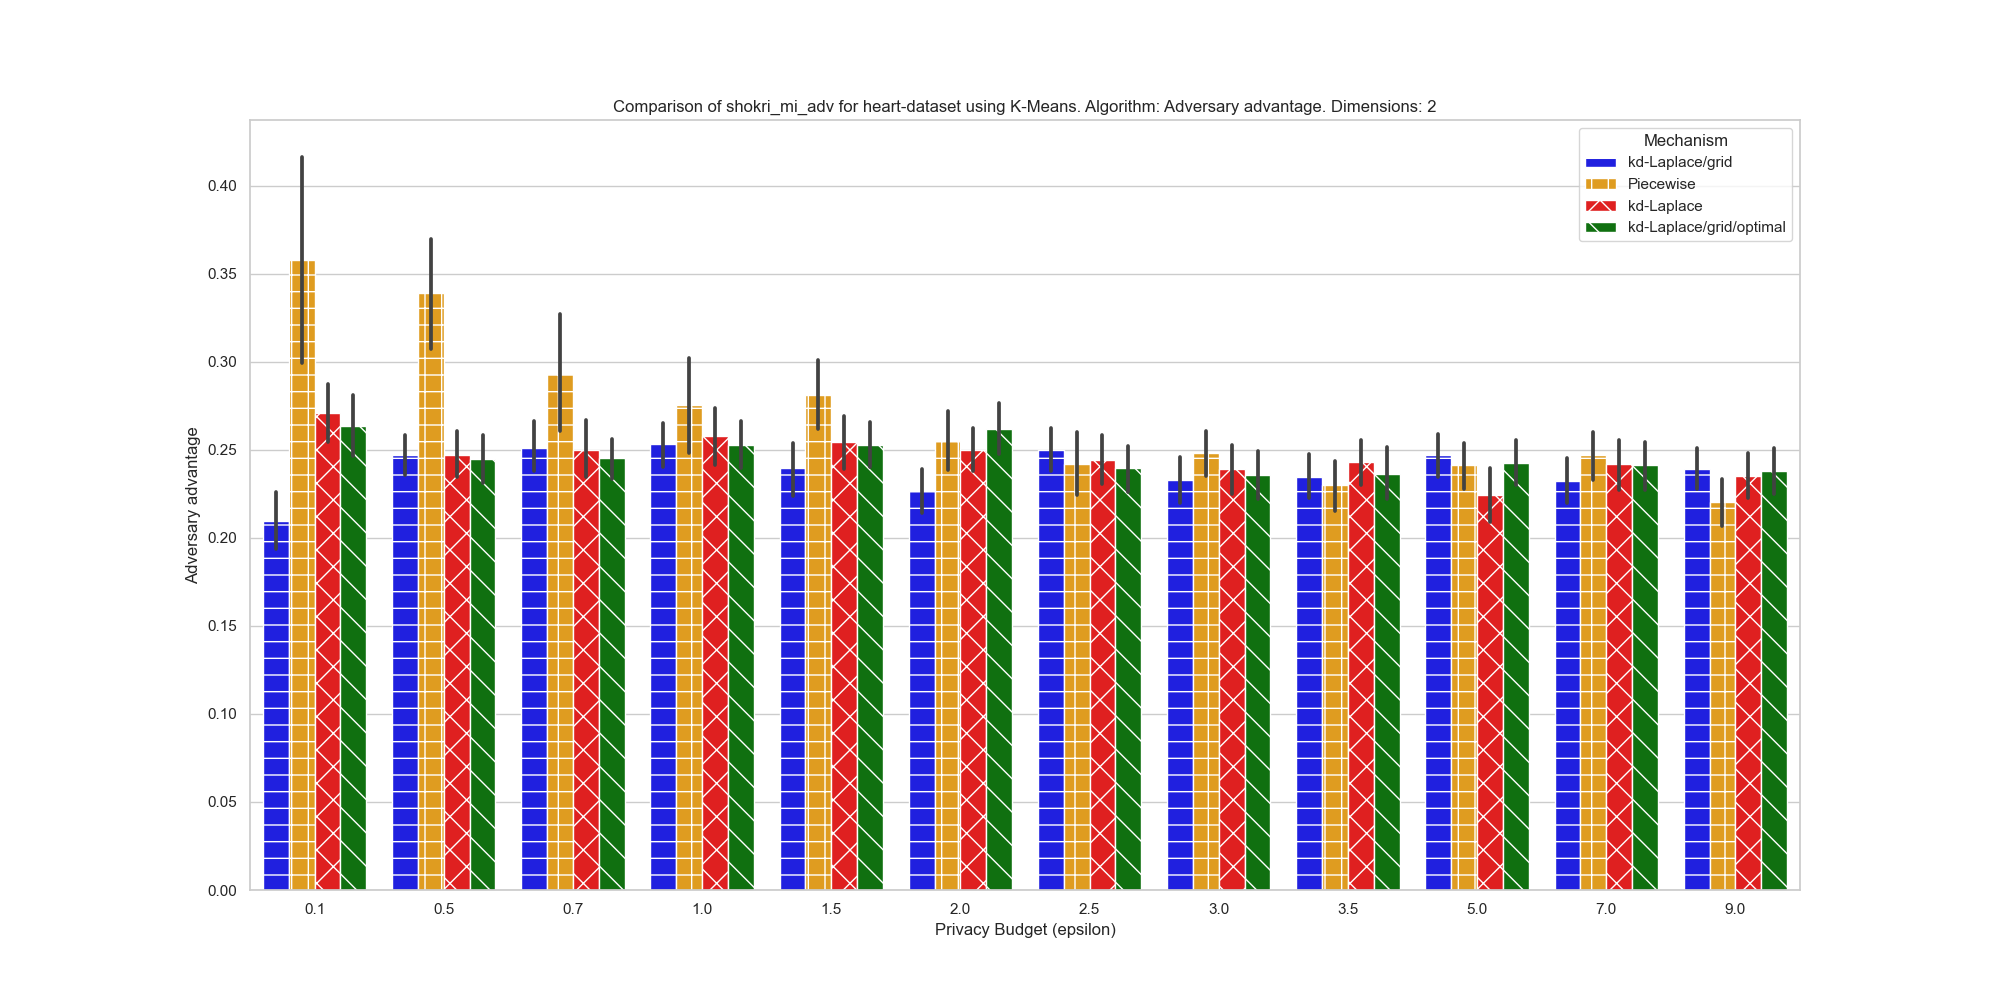
\includegraphics[width=0.50\textwidth]{Results/RQ1/heart-dataset/shokri_mi_adv_heart-dataset_comparison.png}
        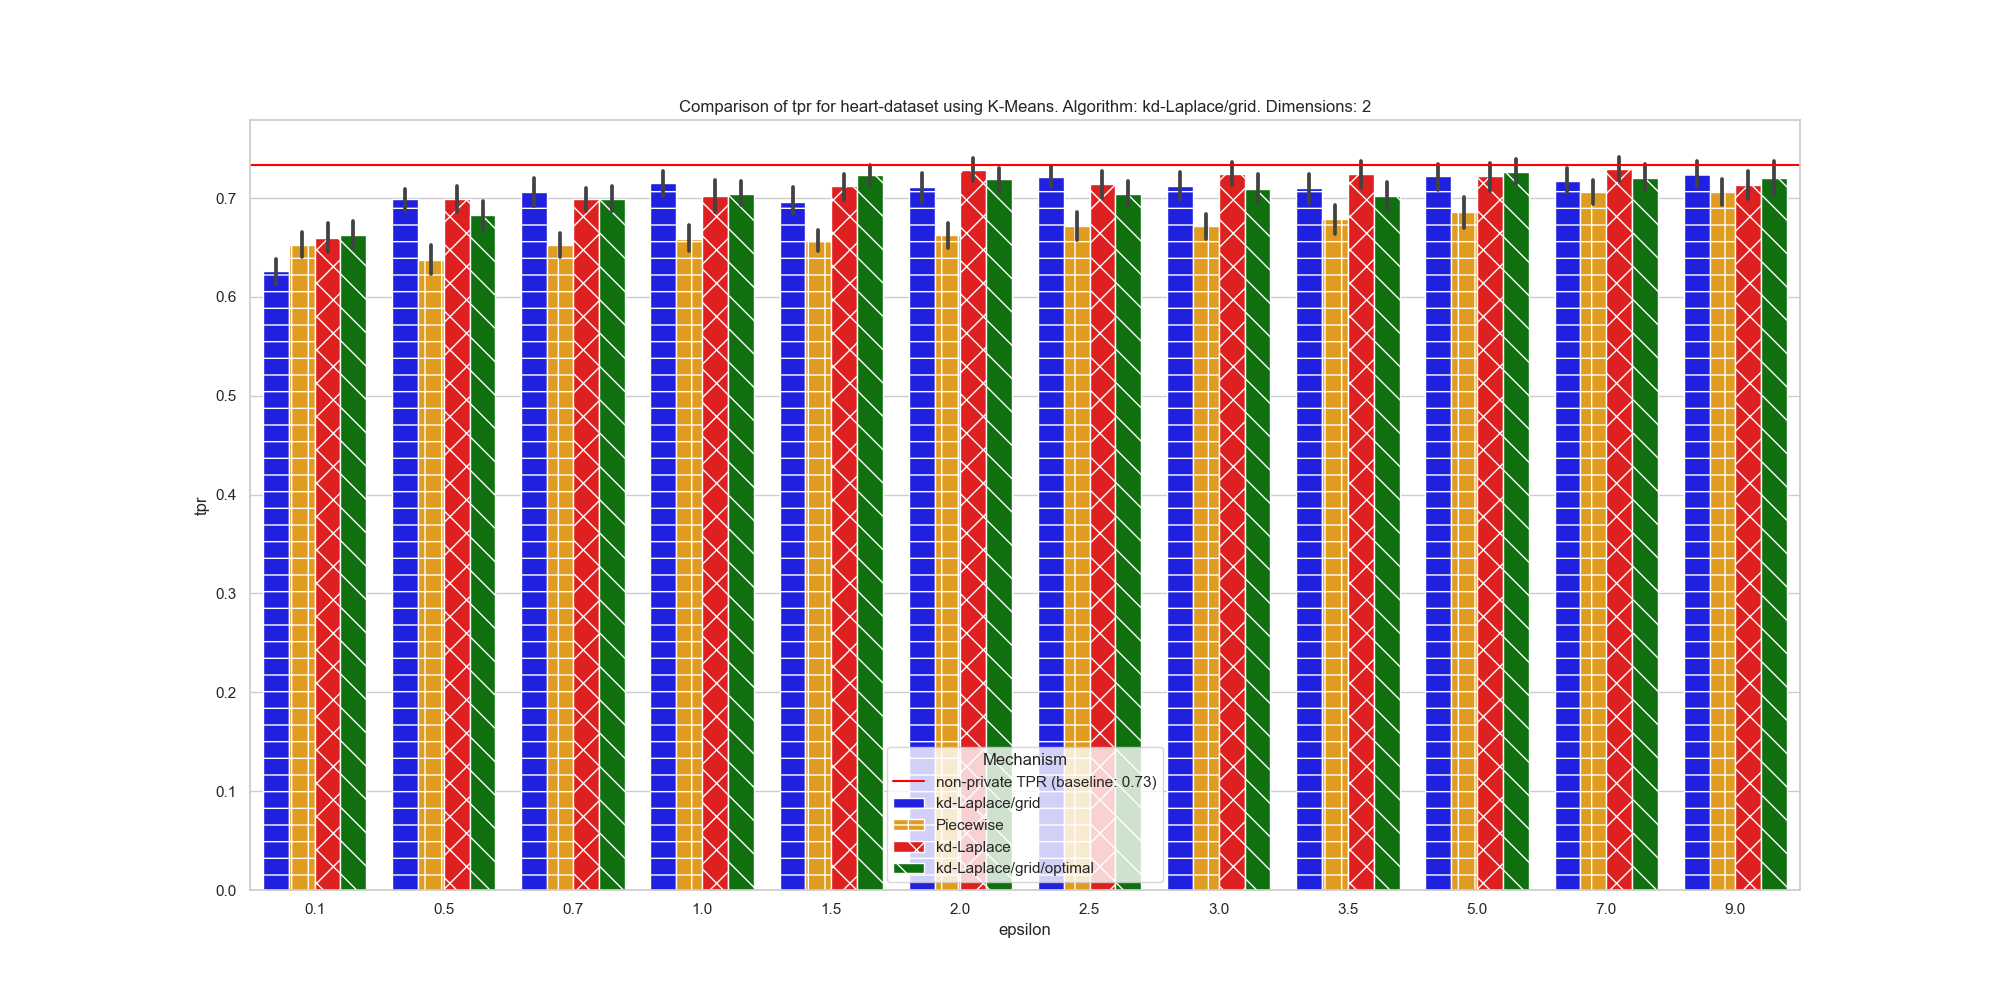
\includegraphics[width=0.50\textwidth]{Results/RQ1/heart-dataset/tpr_heart-dataset_comparison.png}
        \caption{Barplot for adversary advantage (left) and TPR (right) per privacy mechanism for heart-dataset.}
        \label{fig:privacy_heart-dataset_comparison_2d_add_plot}
    \end{minipage}
\end{figure}
The above bar plot shows the adversary advantage based on the membership inference attack. The first graph displays the attack on the seeds dataset, where a clear peak of 0.5 adversary advantage is visible for both Piecewise and kd-Laplace at epsilon 0.1. The other variants of kd-Laplace score similarly, and all fall below 0.2. Piecewise reaches below 0.2 at epsilon 3, while kd-Laplace reaches it at epsilon 2.

For the heart dataset, the difference is slightly smaller, but Piecewise spikes to 0.36 and 0.34 adversary advantage at epsilon 0.1 and 0.5, respectively. Furthermore, kd-Laplace and Piecewise hover around 0.25 adversary advantage for the remaining epsilons.
\newpage
\begin{figure}[H]
    \centering
    \begin{minipage}[c]{\textwidth}
        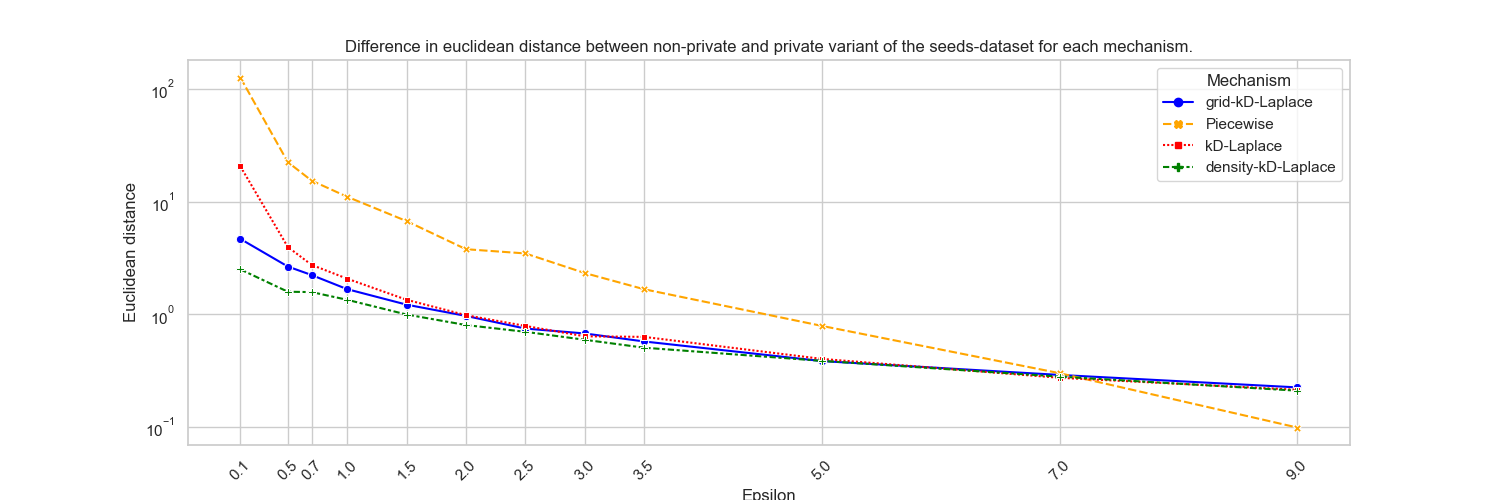
\includegraphics[width=\textwidth]{Results/RQ1/seeds-dataset/privacy_distance_plot.png}
        \caption{Privacy distance for each mechanism for seeds-dataset.}
        \label{fig:privacy_seeds-dataset_comparison_2d_privacy_distance_plot}
    \end{minipage}
    \begin{minipage}[c]{\textwidth}
        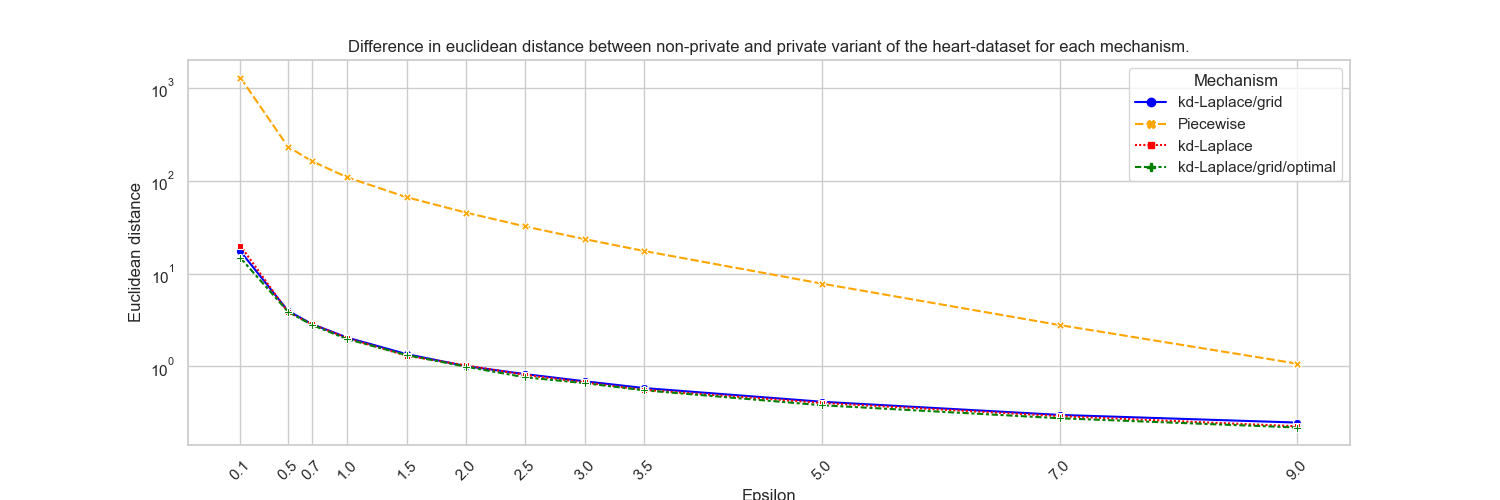
\includegraphics[width=\textwidth]{Results/RQ1/heart-dataset/privacy_distance_plot.png}
        \caption{Privacy distance for each mechanism for heart-dataset.}
        \label{fig:privacy_heart-dataset_comparison_2d_privacy_distance_plot}
    \end{minipage}
\end{figure}
The above graph represents the average Euclidean distance added by each privacy mechanism compared to the two datasets. We use a logarithmic scale for the Euclidean distance to better visualize the results.
For both datasets, the Piecewise mechanism adds the most privacy. When considering the kd-Laplace variants on the seeds dataset, kd-Laplace without optimizations adds the most distance, followed by kd-Laplace/grid and kd-Laplace/grid/optimal. For the heart dataset, all variants of kd-Laplace are nearly equal.
\newpage
\subsection{3-dimensional data}
\begin{figure}[H]
    \centering
    \begin{minipage}[c]{1.1\textwidth}
        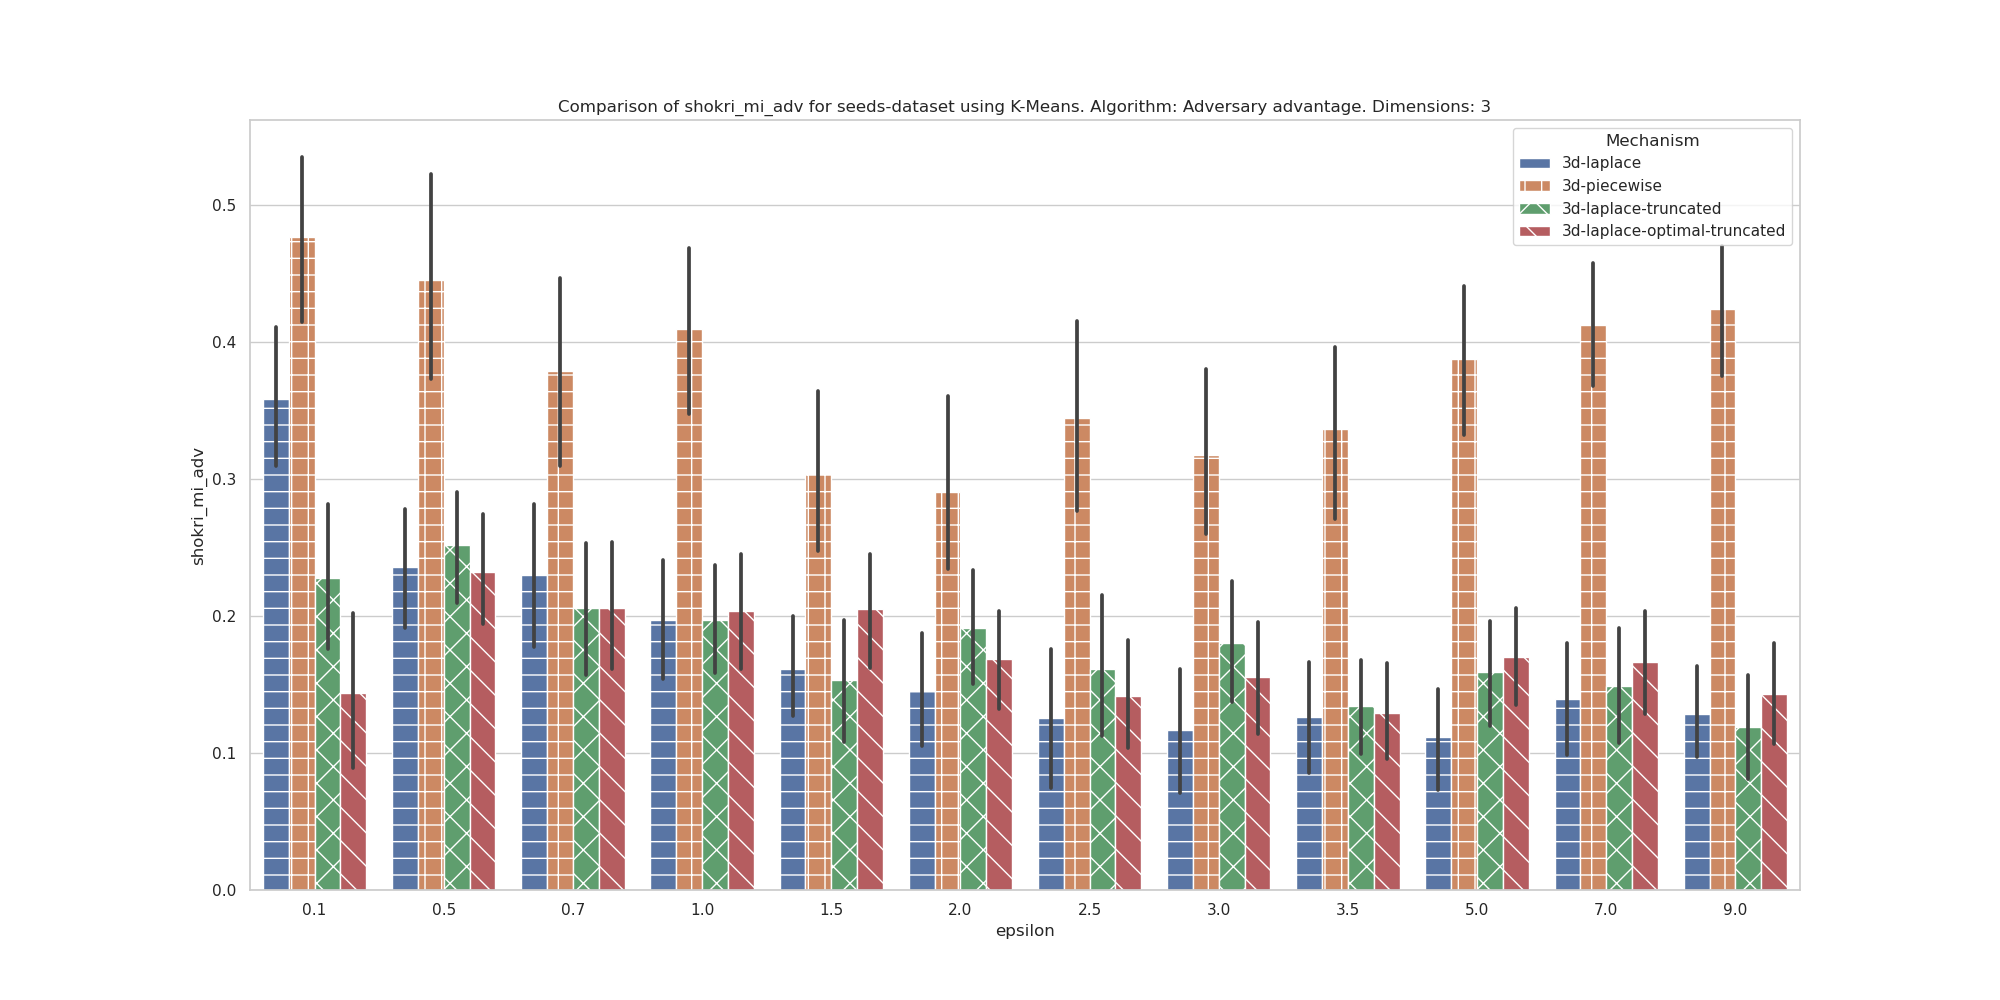
\includegraphics[width=0.50\textwidth]{Results/RQ2/seeds-dataset/shokri_mi_adv_seeds-dataset_comparison.png}
        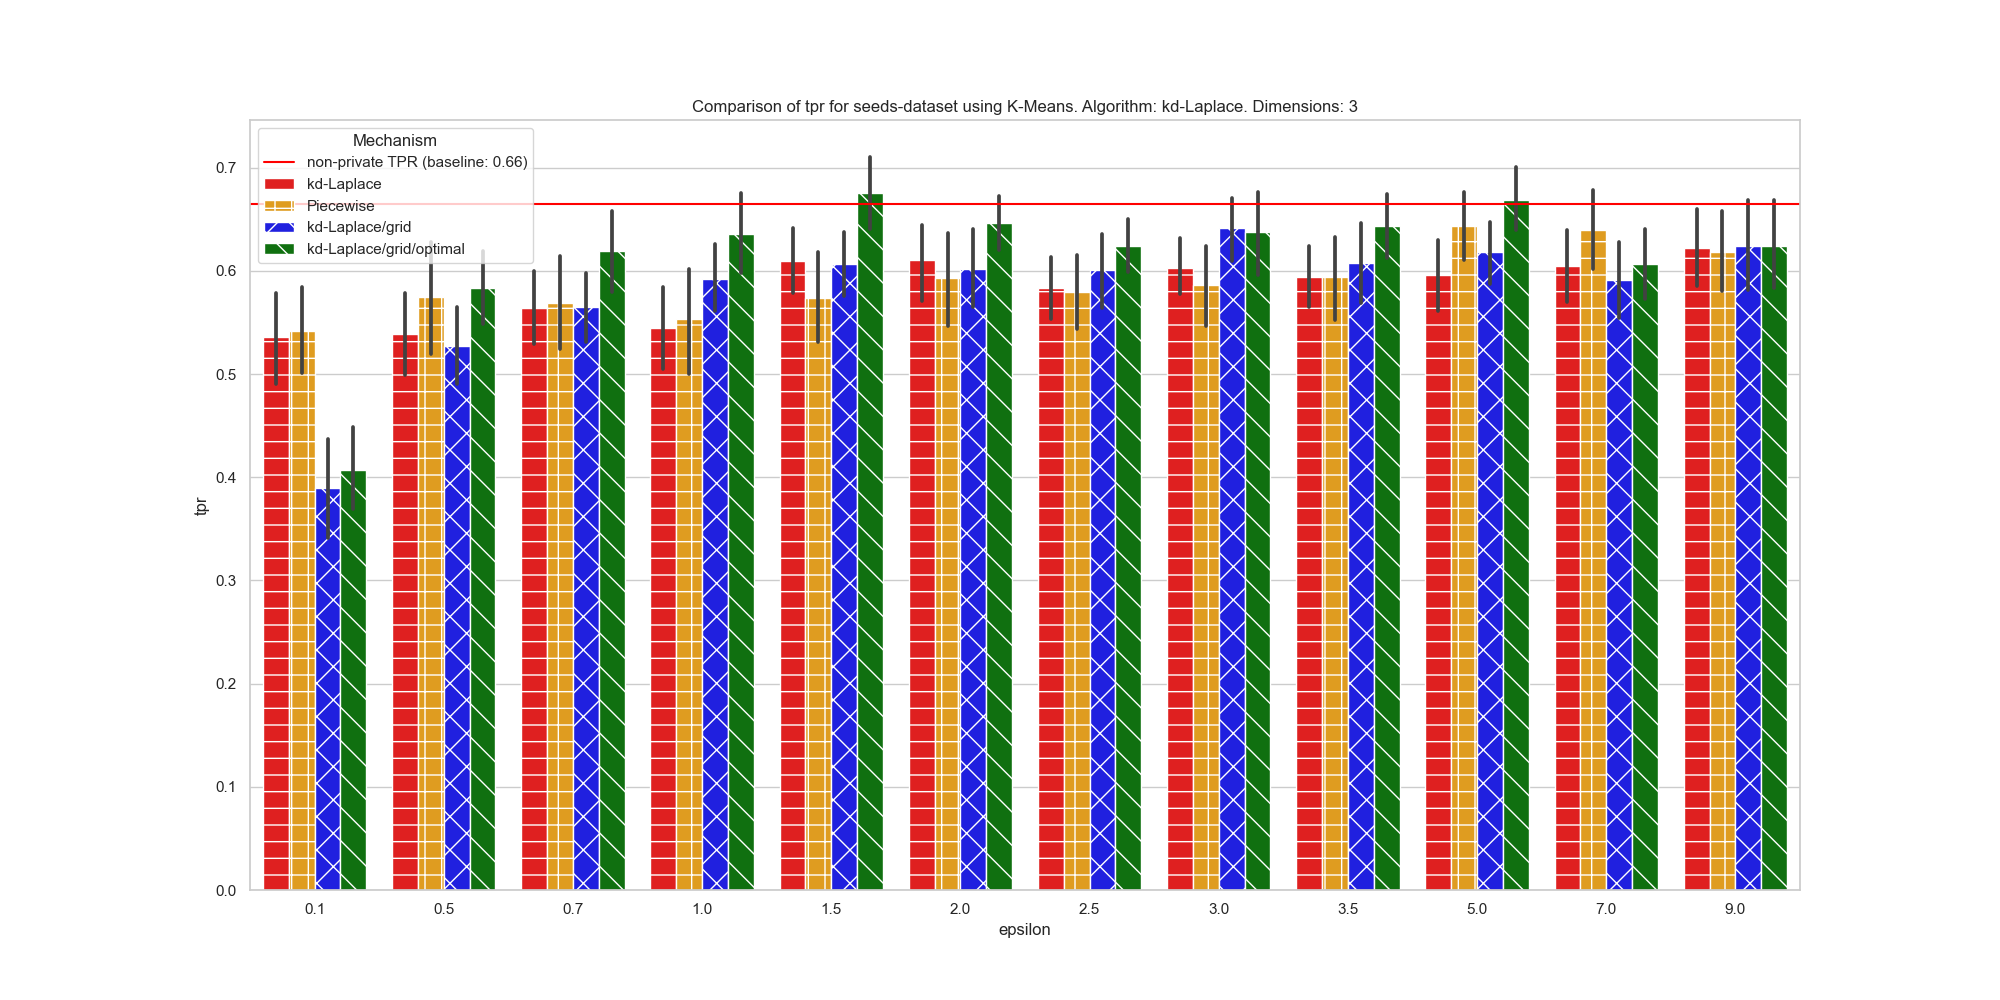
\includegraphics[width=0.50\textwidth]{Results/RQ2/seeds-dataset/tpr_seeds-dataset_comparison.png}
        \caption{Barplot for adversary advantage (left) and TPR (right) per privacy mechanism for seeds-dataset.}
        \label{fig:privacy_seeds-dataset_comparison_3d_aa_plot}
    \end{minipage}
    \begin{minipage}[c]{1.1\textwidth}
        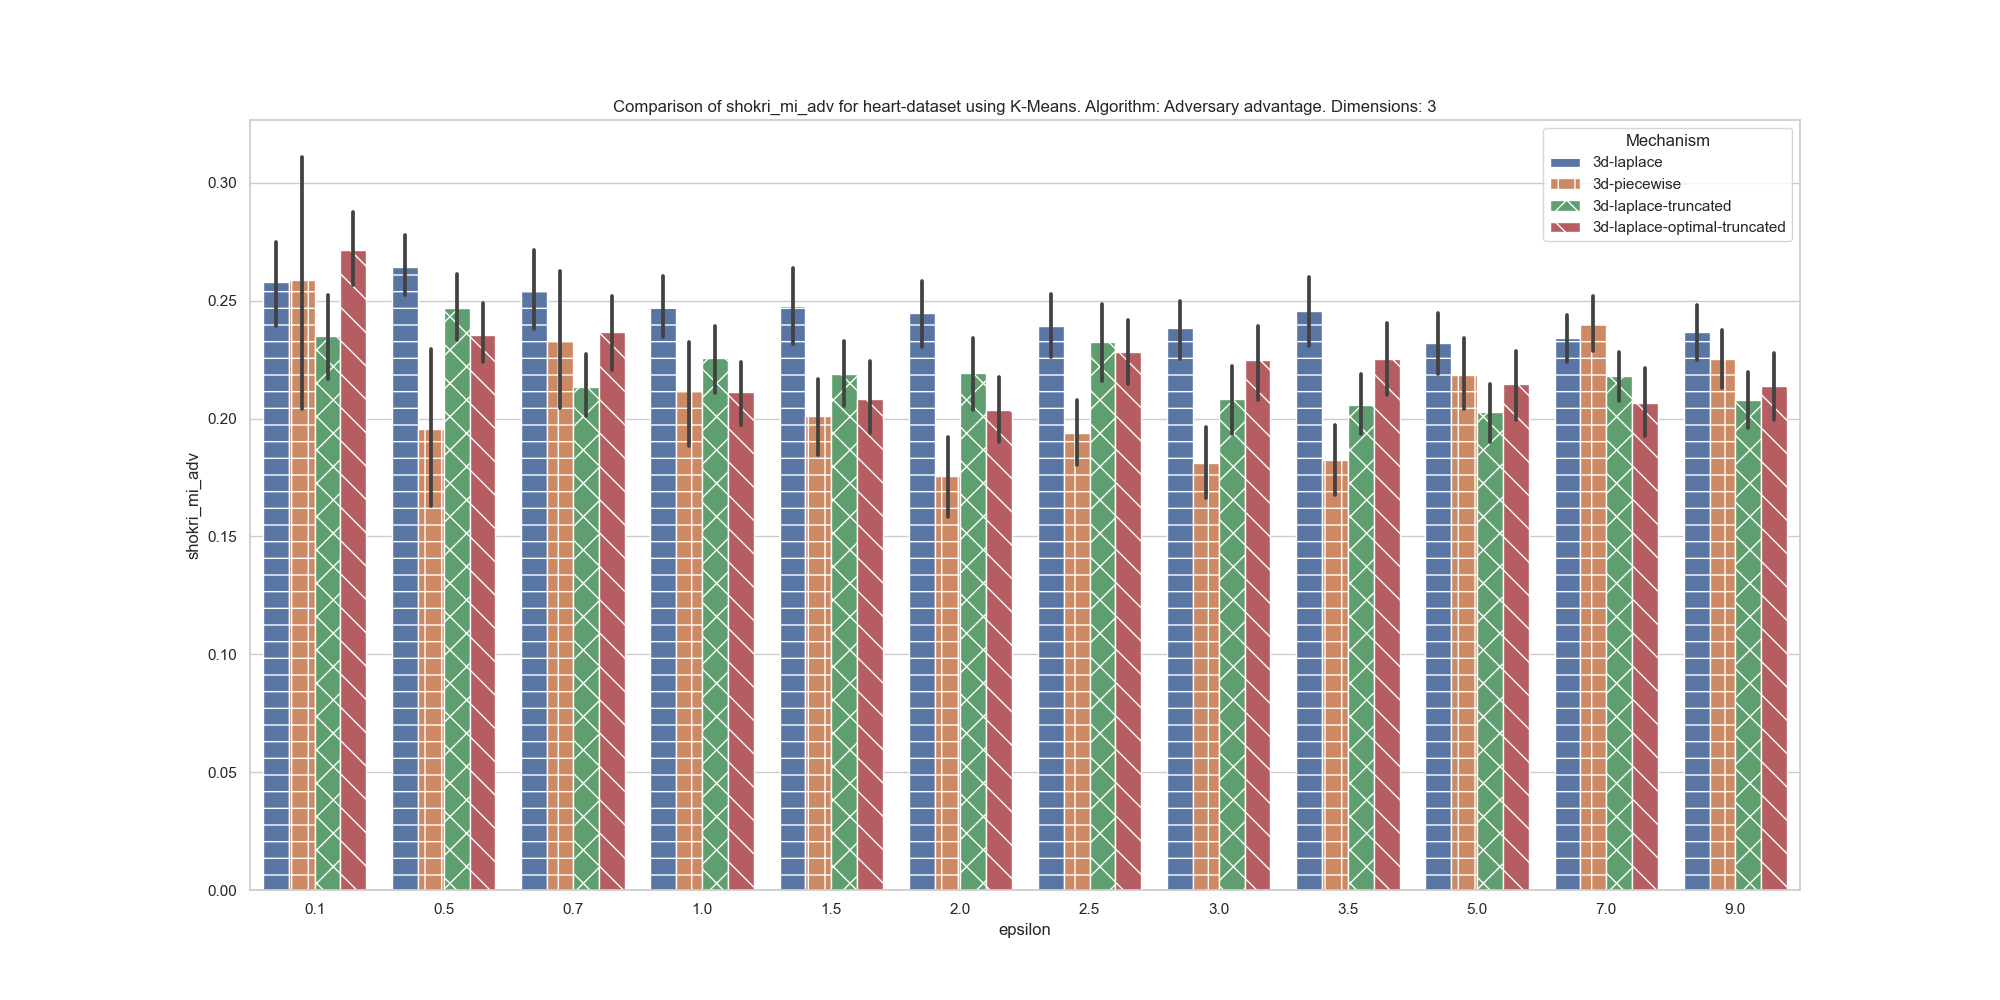
\includegraphics[width=0.50\textwidth]{Results/RQ2/heart-dataset/shokri_mi_adv_heart-dataset_comparison.png}
        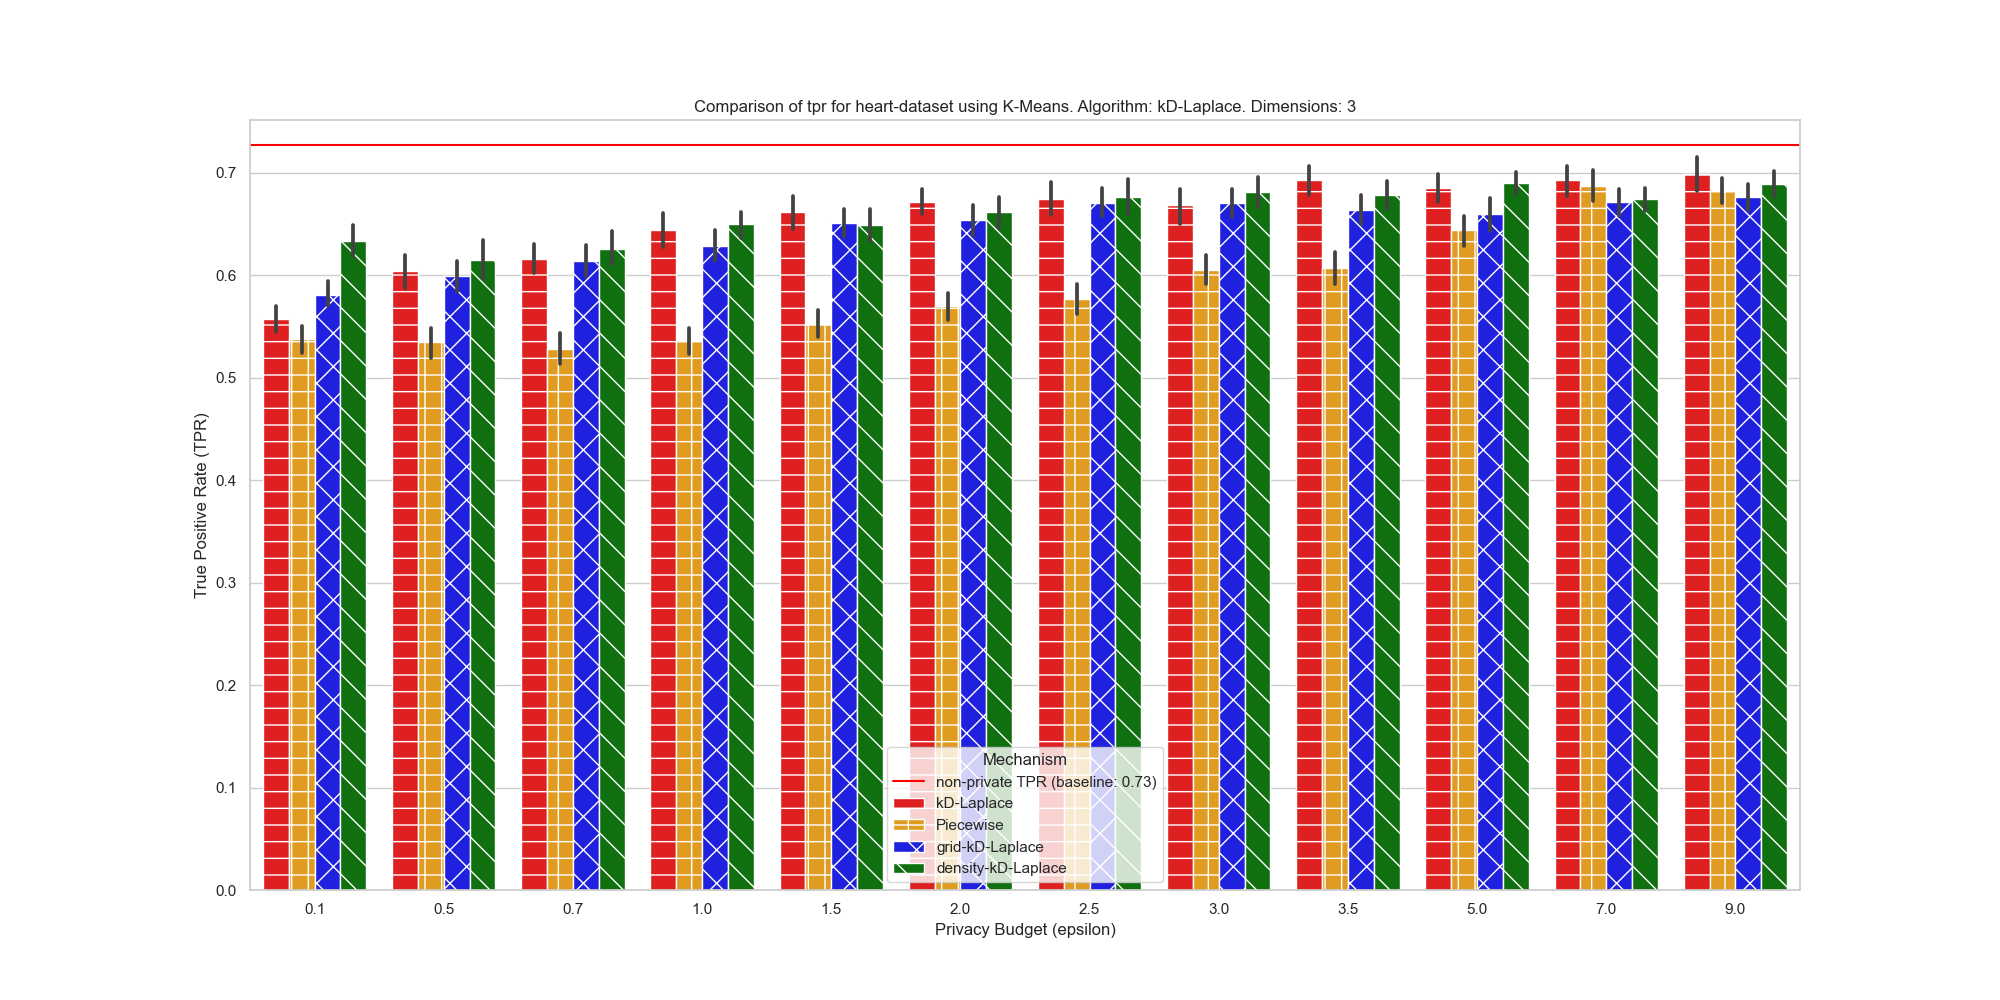
\includegraphics[width=0.50\textwidth]{Results/RQ2/heart-dataset/tpr_heart-dataset_comparison.png}
        \caption{Barplot for adversary advantage (left) and TPR (right) per privacy mechanism for heart-dataset.}
        \label{fig:privacy_heart-dataset_comparison_3d_aa_plot}
    \end{minipage}
\end{figure}
The graphs above show the adversary advantage (left) and TPR (right) for the seeds dataset (top) and heart dataset (bottom).
The first dataset we analyze is the seeds dataset. We can observe a clear pattern for the Piecewise mechanism based on the adversary advantage plot for the seeds dataset. It scores between 0.4 and 0.5 for epsilon values ranging from 0.1 to 0.7 and drops below 0.2 for epsilon values higher than 3.
The kd-Laplace mechanism, particularly the variant without optimizations (red), has a high adversary advantage (0.35) for epsilon 0.1. After that, all kd-Laplace variants perform similarly. When we compare them to the TPR, we still see that Piecewise and the regular kd-Laplace variant have higher scores for epsilon 0.1 (0.5+). After that, the mechanisms perform similarly, but we notice that kd-Laplace/grid/optimal consistently outperforms the others. Additionally, the latter is above the baseline value for epsilon 1.5.

Now, let's turn our attention to the heart dataset. Here, we can see that the adversary advantage shows less variation than the seeds dataset. For all epsilon values, kd-Laplace without optimizations stands out. The mechanisms perform similarly, but the Piecewise mechanism performs better for epsilon values between 1.5 and 5.0.
For the TPR, all mechanisms are below the baseline value. They score the same, but the Piecewise mechanism is approximately 0.05 TPR lower than the kd-Laplace variants for epsilon values 0.1 to 3.5.
\newpage
\begin{figure}[H]
    \centering
    \begin{minipage}[c]{1\textwidth}
        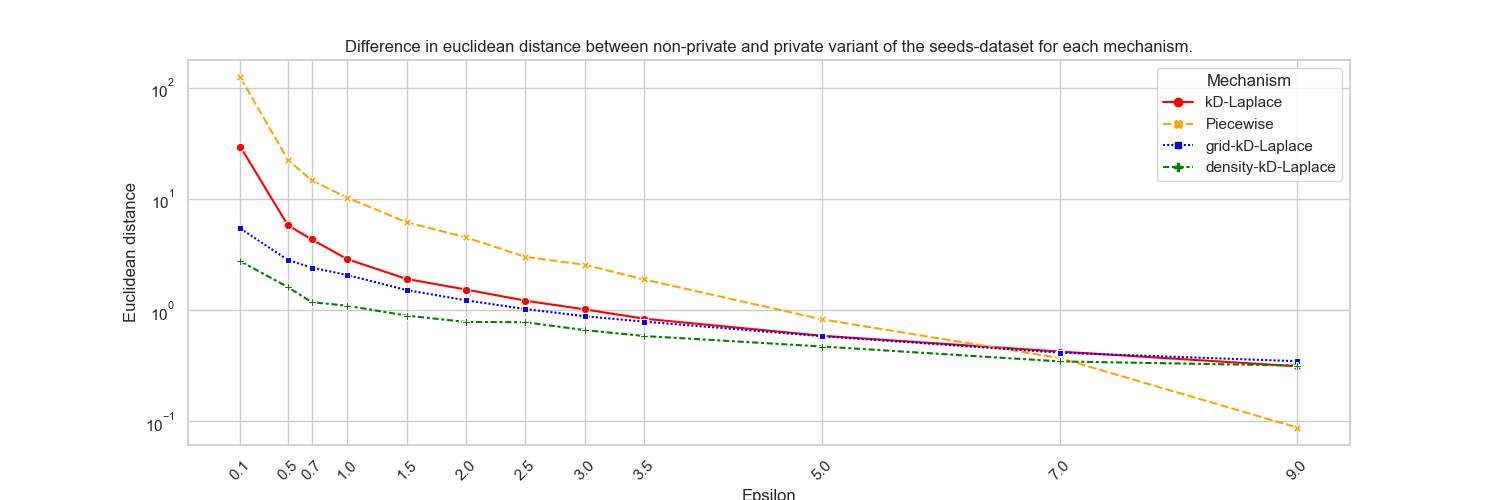
\includegraphics[width=1\textwidth]{Results/RQ2/seeds-dataset/privacy_distance_plot.png}
        \caption{Privacy distance for each mechanism for 3D seeds-dataset.}
        \label{fig:privacy_seeds-dataset_comparison_3d_privacy_distance_plot}
    \end{minipage}
    \begin{minipage}[c]{1\textwidth}
        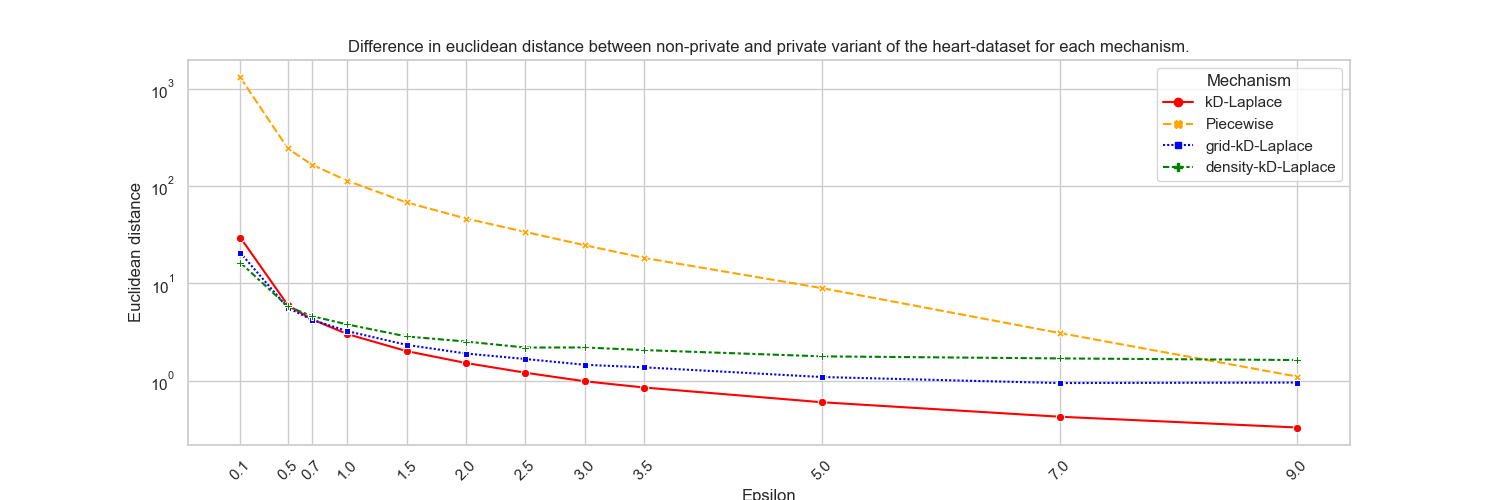
\includegraphics[width=1\textwidth]{Results/RQ2/heart-dataset/privacy_distance_plot.png}
        \caption{Privacy distance for each mechanism for 3D heart-dataset.}
        \label{fig:privacy_heart-dataset_comparison_3d_privacy_distance_plot}
    \end{minipage}
\end{figure}
%#The above graphs depict the average Euclidean distances between the data with privacy mechanisms applied and without them for the seeds dataset (top) and heart dataset (bottom). 
%A clear distinction can be observed among the different distances for the seeds dataset. On average, the Piecewise mechanism adds the most distance. 
At epsilon values 7 and 9, the Piecewise mechanism adds the least distance. Among the various kd-Laplace variants, the variant without optimizations adds the most distance.
This trend continues until epsilon 5, after which the variants become equal.

Similarly, a noticeable difference is observed between the Piecewise mechanism and kd-Laplace for the heart dataset. At epsilon 9, the Piecewise mechanism has the same score as kd-Laplace.
Among the kd-Laplace variants, the variant without optimizations adds the least distance, but it is slightly higher than the other variants for epsilon 0.1.
\newpage
%\subsection{Utility}
%subsubsection*{Cluster comparison}
%\todo[inline]{Add plot}
%\subsubsection*{Mechanism comparison}
%\begin{figure}[H]
%    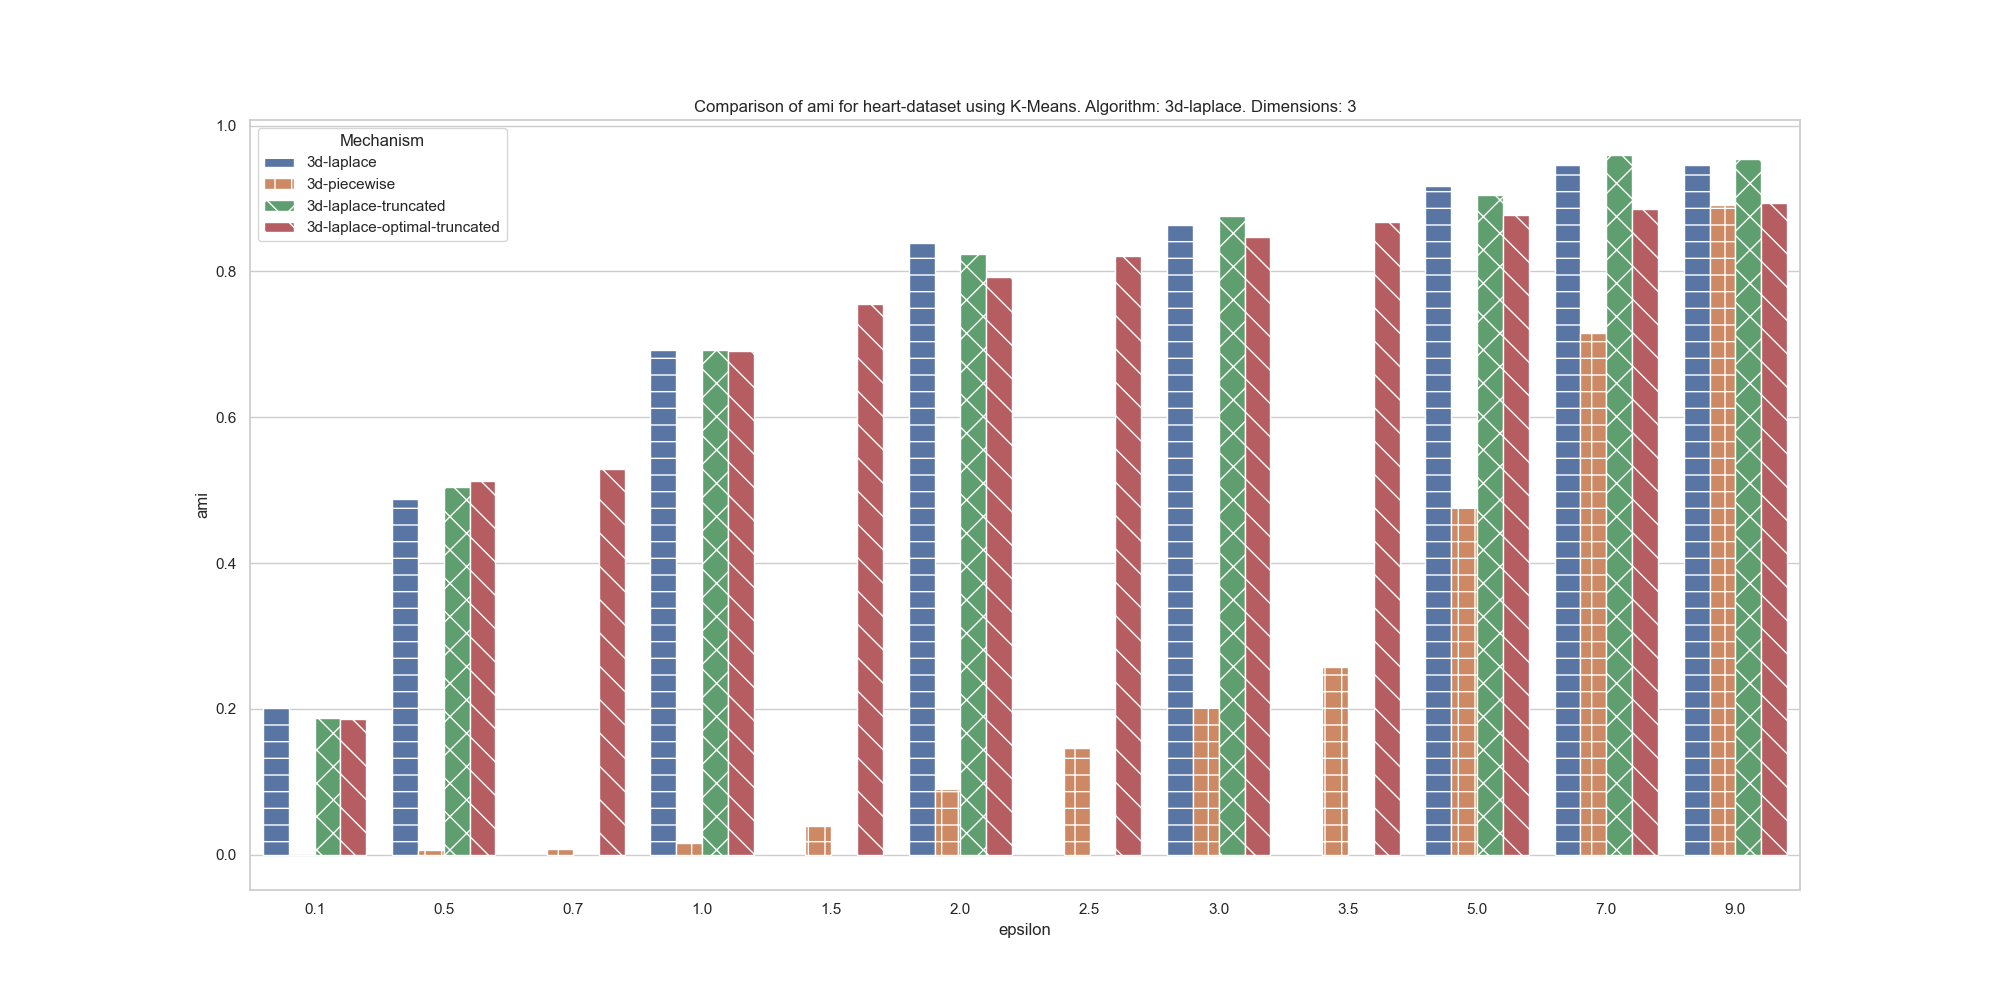
\includegraphics[width=\textwidth]{Results/RQ2/heart-dataset/ami_heart-dataset_comparison.png}
%    \caption{Adjusted Mutual Information comparison for the 3-dimensional heart-dataset}
%    \label{fig:ami_heart-dataset_comparison_3d}
%\end{figure}
%\begin{figure}[H]
%    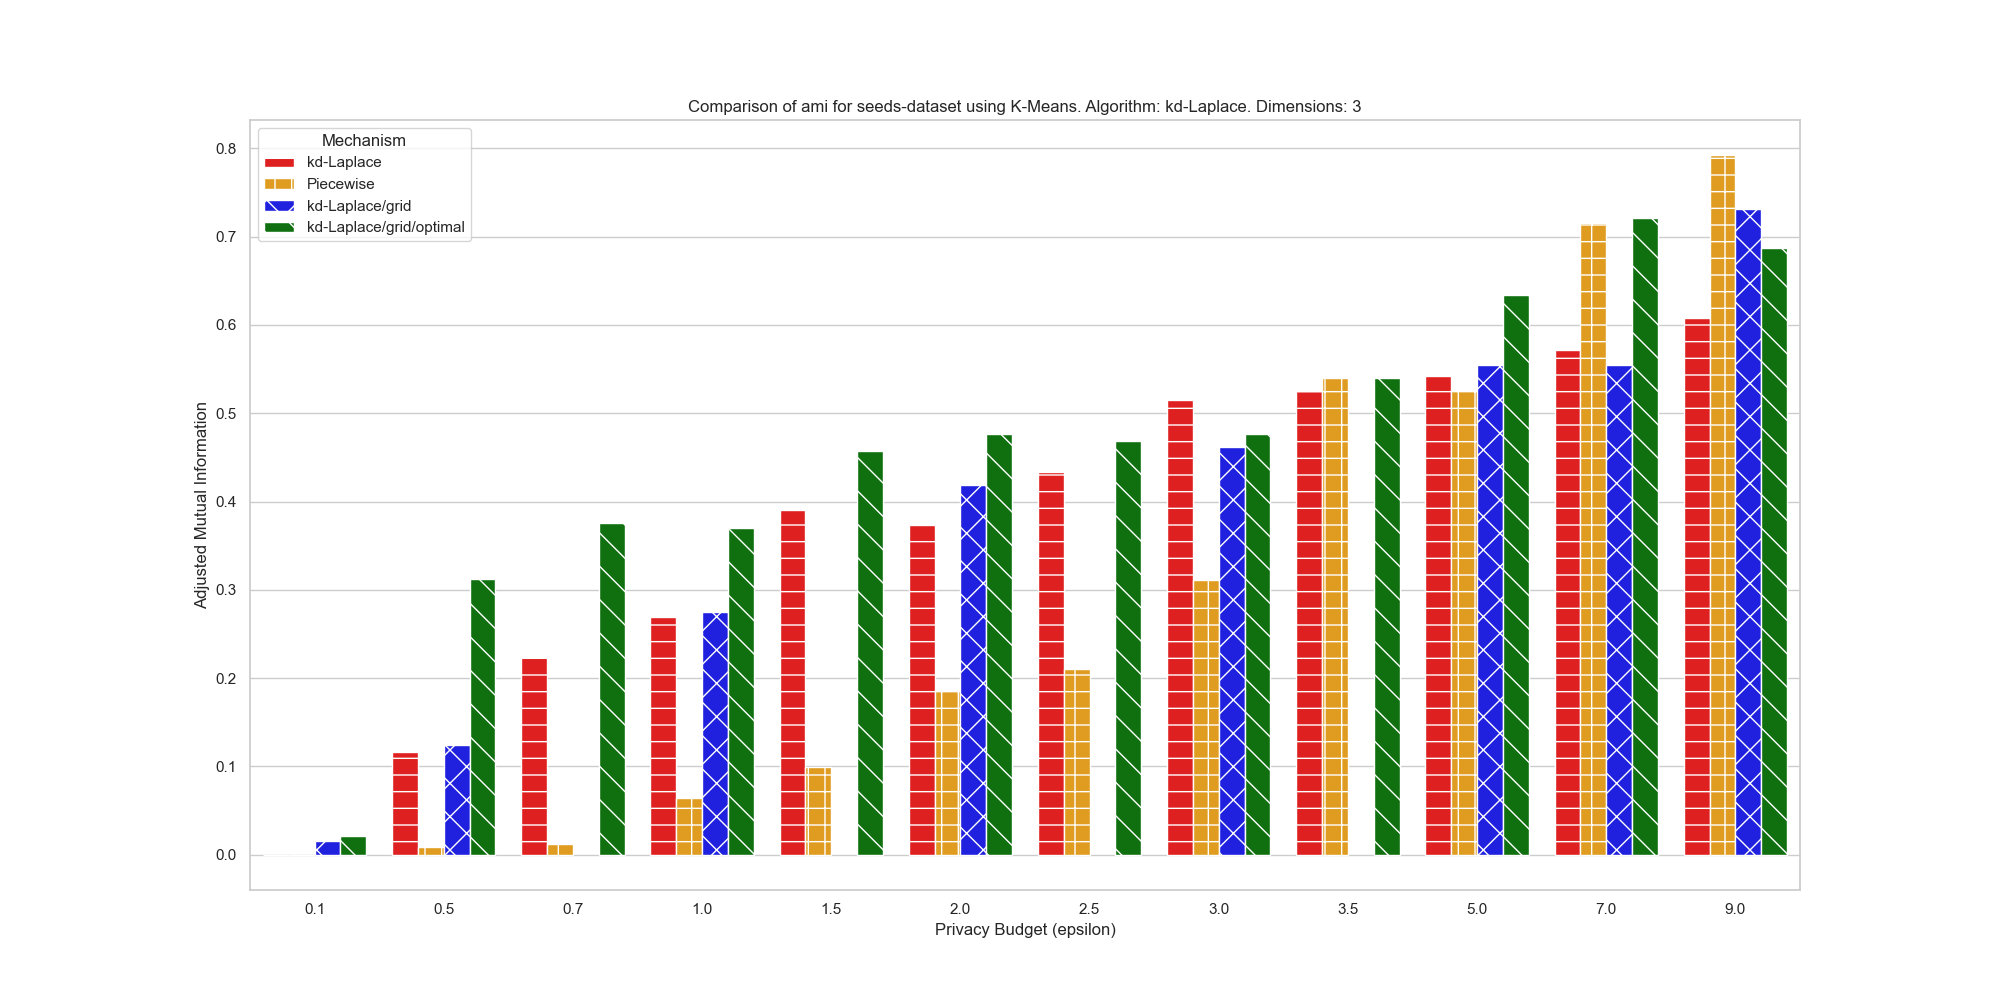
\includegraphics[width=\textwidth]{Results/RQ2/seeds-dataset/ami_seeds-dataset_comparison.png}
%    \caption{Adjusted Mutual Information comparison for the 3-dimensional seeds-dataset}
%    \label{fig:ami_seeds-dataset_comparison_3d}
%\end{figure}
%\todo[inline]{Add links to scilliouette plots and other plots}
\subsection{n-dimensional data}
\begin{figure}[H]
    \centering
    \begin{minipage}[c]{1.1\textwidth}
        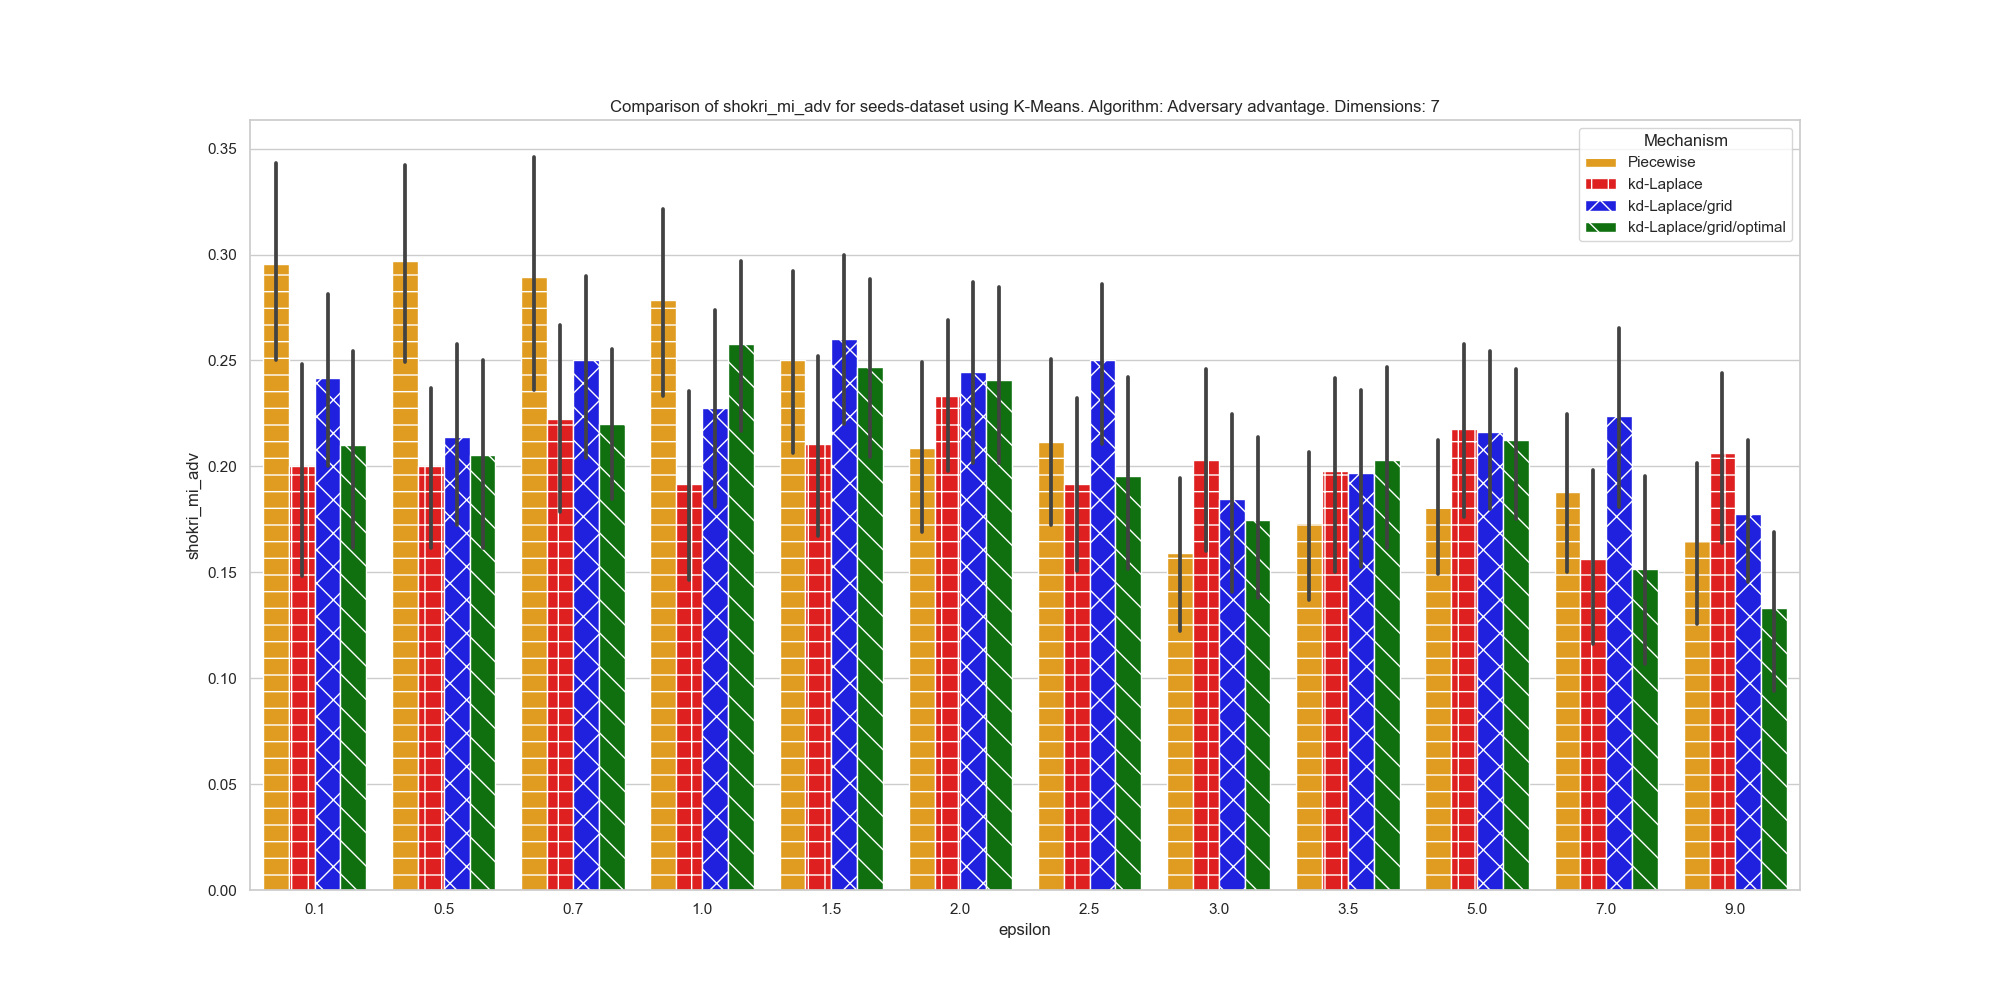
\includegraphics[width=0.50\textwidth]{Results/RQ2-nd/seeds-dataset/shokri_mi_adv_seeds-dataset_comparison.png}
        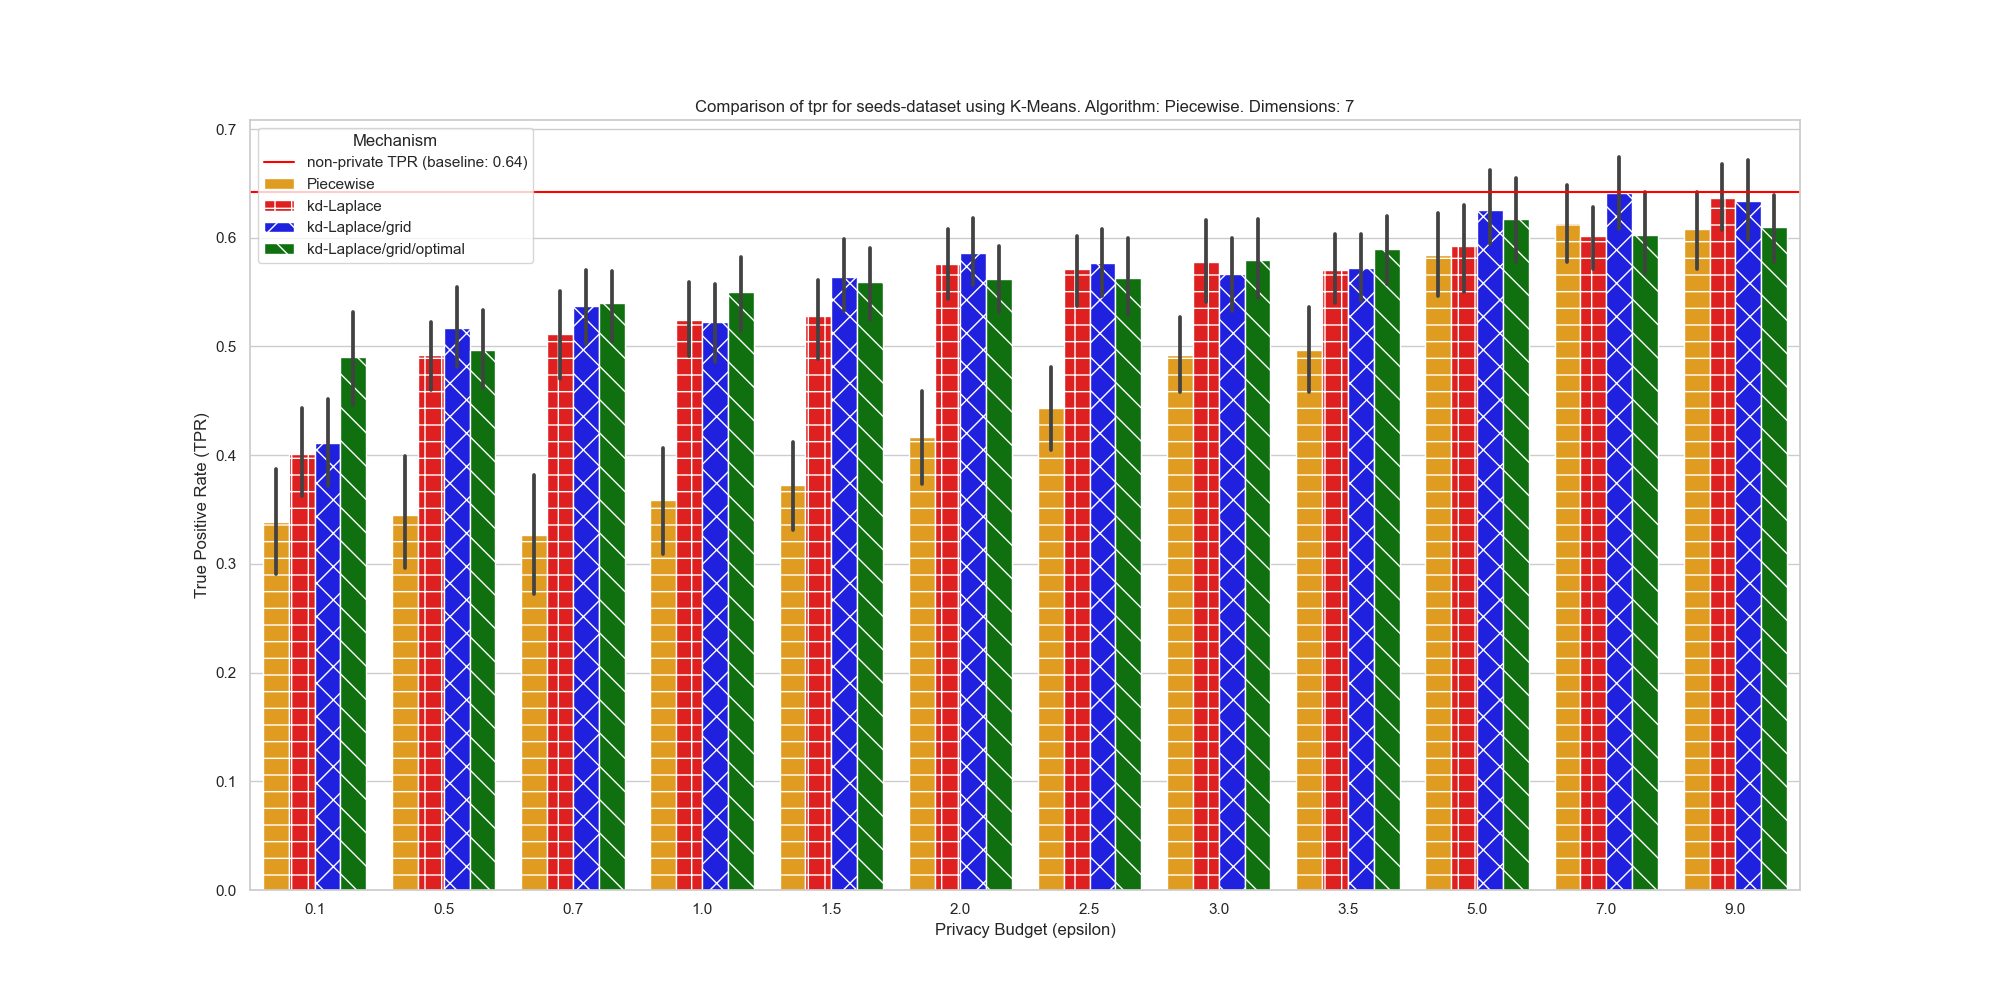
\includegraphics[width=0.50\textwidth]{Results/RQ2-nd/seeds-dataset/tpr_seeds-dataset_comparison.png}
        \caption{Barplot for adversary advantage (left) and TPR (right) per privacy mechanism for seeds-dataset.}
        \label{fig:privacy_seeds-dataset_comparison_nd_aa_plot}
    \end{minipage}
    \begin{minipage}[c]{1.1\textwidth}
        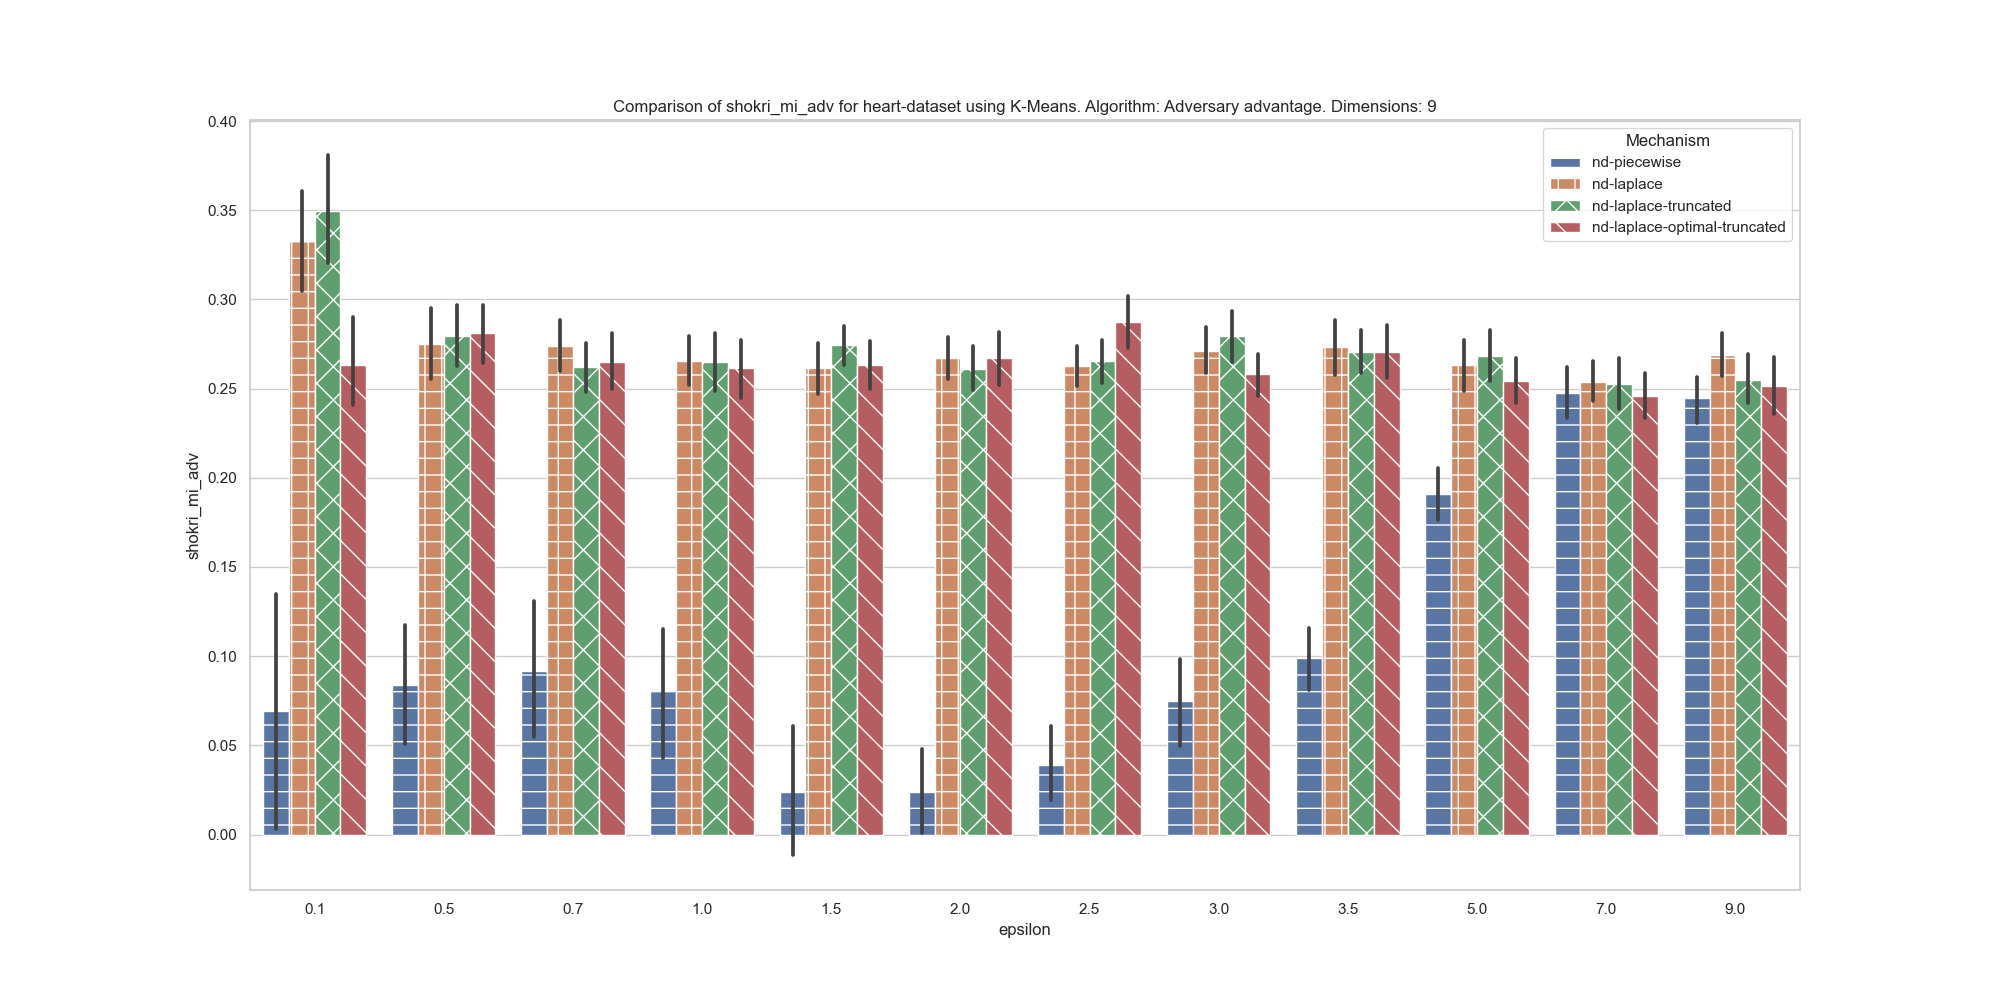
\includegraphics[width=0.50\textwidth]{Results/RQ2-nd/heart-dataset/shokri_mi_adv_heart-dataset_comparison.png}
        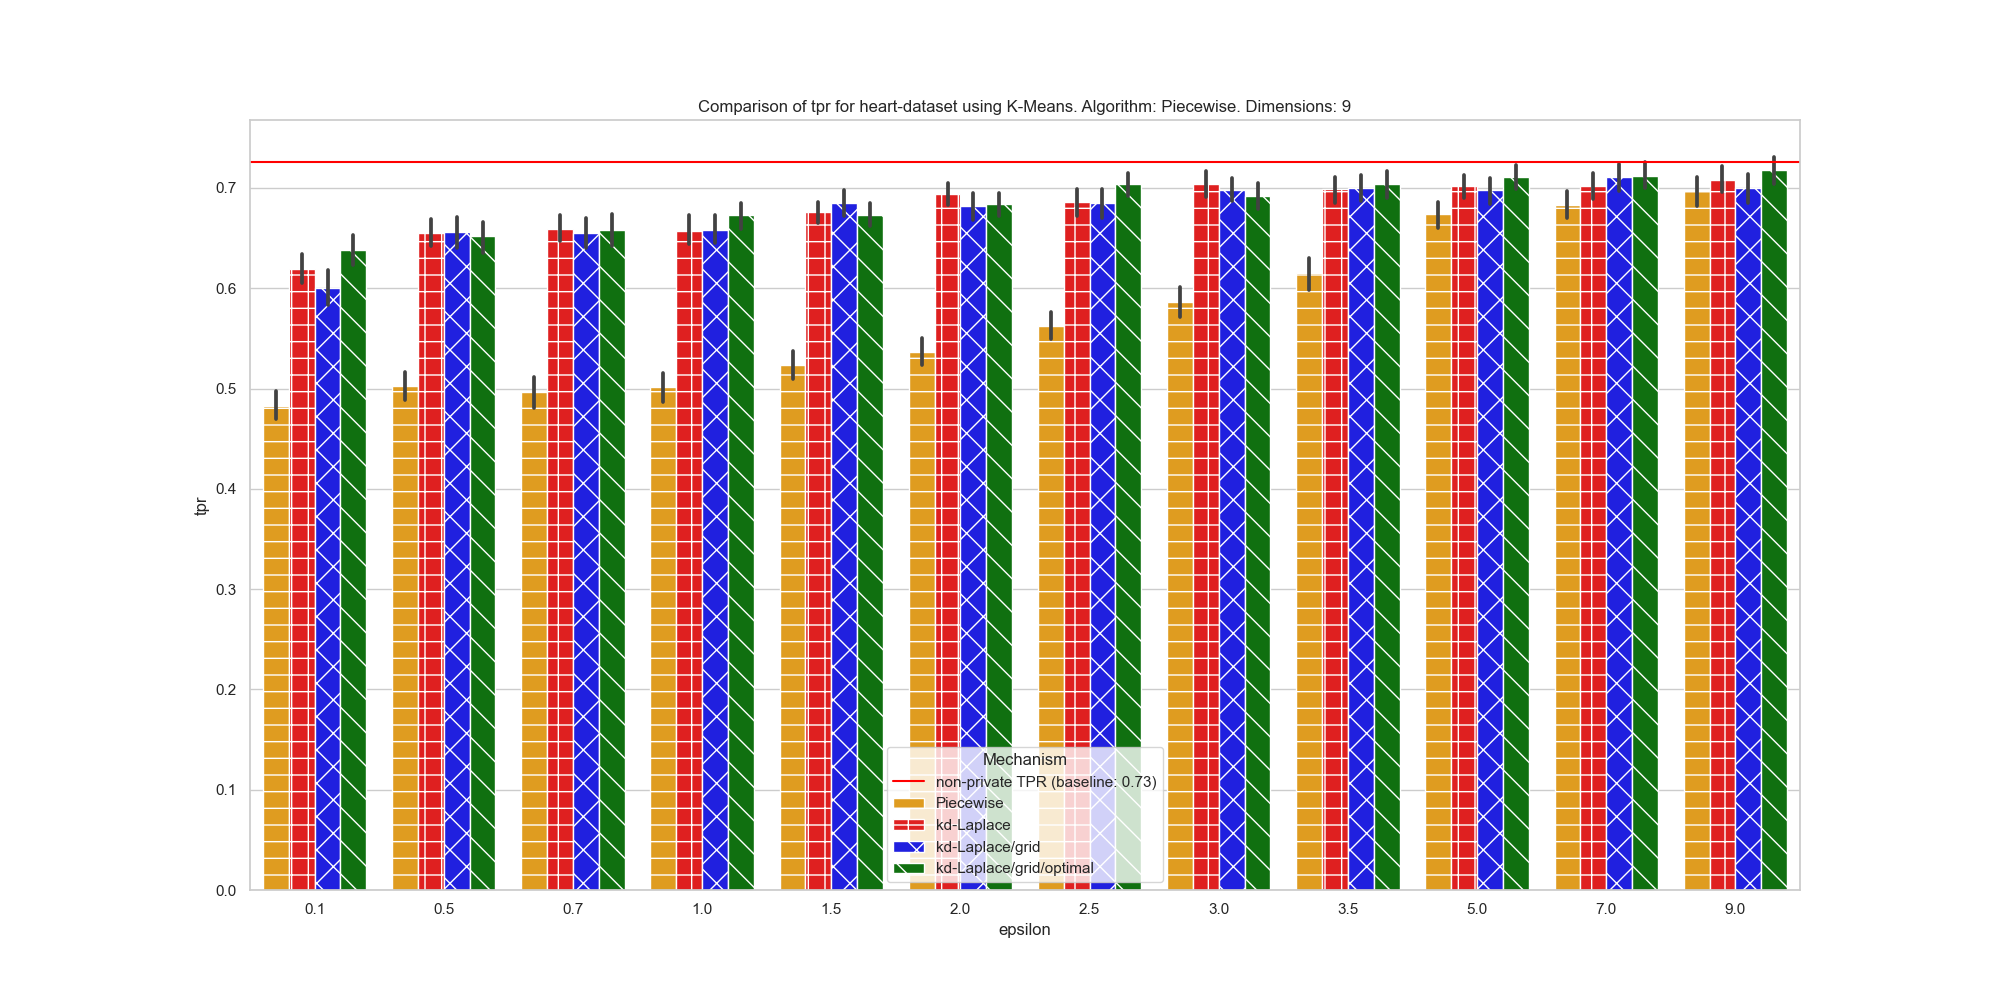
\includegraphics[width=0.50\textwidth]{Results/RQ2-nd/heart-dataset/tpr_heart-dataset_comparison.png}
        \caption{Barplot for adversary advantage (left) and TPR (right) per privacy mechanism for heart-dataset.}
        \label{fig:privacy_heart-dataset_comparison_nd_aa_plot}
    \end{minipage}
\end{figure}
%The above graphs display the adversary advantage (left) and TPR (right) per epsilon for the seeds dataset (top) and heart dataset (bottom).

The seeds dataset shows that Piecewise has a higher adversary advantage for epsilons ranging from 0.1 to 1.
However, the TPR for Piecewise is consistently lower than that of kd-Laplace. There is no clear distinction among the kd-Laplace variants.
However, for epsilon values 7 and 9, kd-Laplace/grid/optimal does not exceed the baseline for TPR, while the other variants do.

For the heart dataset, the Piecewise mechanism scores below 0.10 for adversary advantage for epsilons 0.1 to 3.
In contrast, the kd-Laplace variants yield values above 0.25 for the same epsilon values.
The Piecewise mechanism also scores lower for epsilon values 3.5 and 5, but they have nearly equal scores for epsilons 7 and 9.
Among the variants of kd-Laplace, kd-Laplace, and kd-Laplace/grid perform slightly worse for epsilon 0.1, but for the other epsilons, they function similarly.
The TPR follows a similar trend to the adversary advantage, except for epsilon 0.1, where the kd-Laplace variants have equal scores.

\newpage
%\begin{tabular}{llrr}
\toprule
 &  & True Positive Rate & False Positive Rate \\
algorithm & epsilon &  &  \\
\midrule
\bottomrule
\end{tabular}


\begin{figure}[H]
    \centering
    \begin{minipage}[c]{0.80\textwidth}
        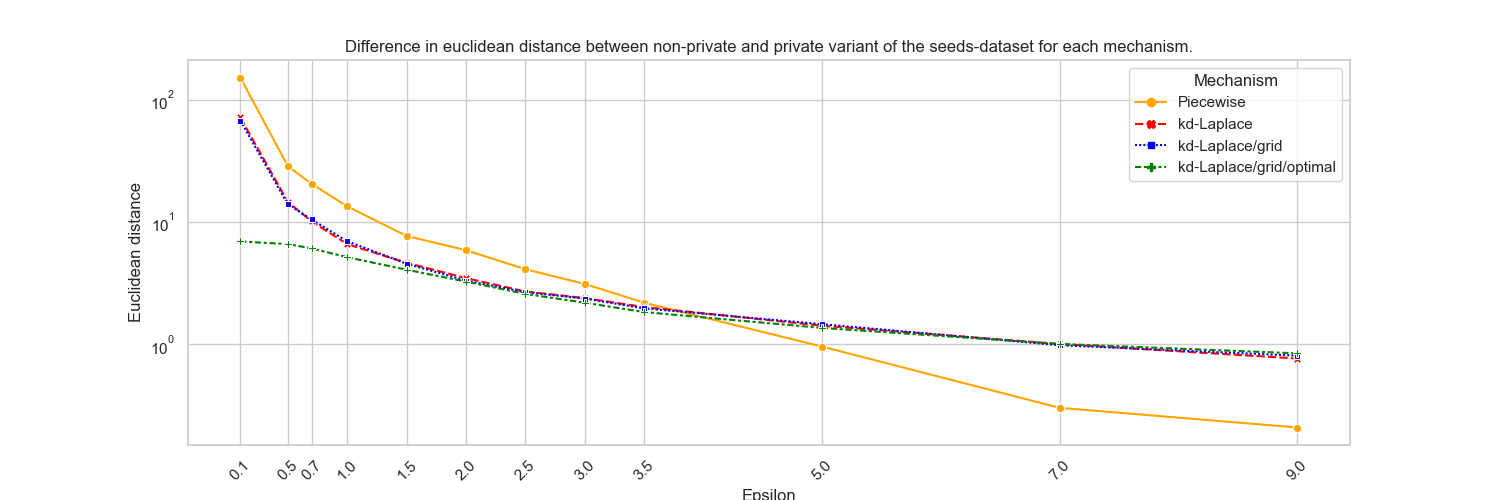
\includegraphics[width=1\textwidth]{Results/RQ2-nd/seeds-dataset/privacy_distance_plot.png}
        \caption{Privacy distance for each mechanism for nD seeds-dataset.}
        \label{fig:privacy_seeds-dataset_comparison_nd_privacy_distance_plot}
    \end{minipage}
    \begin{minipage}[c]{0.80\textwidth}
        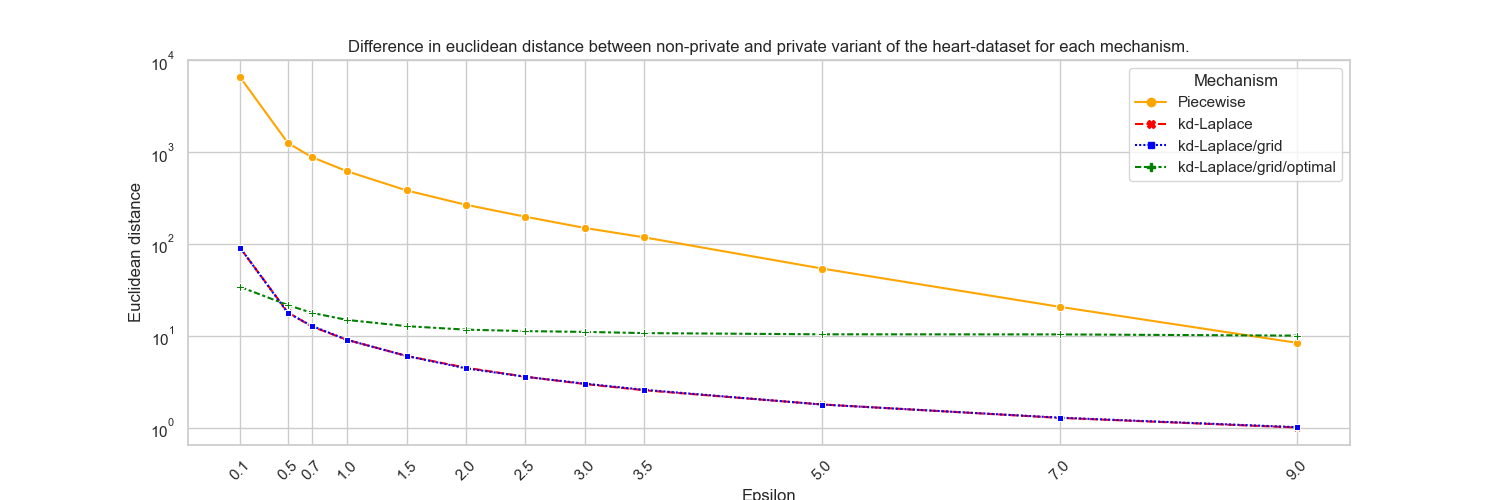
\includegraphics[width=1\textwidth]{Results/RQ2-nd/heart-dataset/privacy_distance_plot.png}
        \caption{Privacy distance for each mechanism for nD heart-dataset.}
        \label{fig:privacy_heart-dataset_comparison_nd_privacy_distance_plot}
    \end{minipage}
\end{figure}
The Piecewise mechanism for epsilon 0.1 to 3.5 for the seeds dataset adds the most Euclidean distance. After that, the Piecewise mechanism decreases significantly and scores lower than the kd-Laplace variants. For kd-Laplace/grid/optimal, the privacy distance starts lowest up to epsilon 1.5. After that, the variants of the kd-Laplace score are almost the same.

For the heart dataset, the Piecewise mechanism also adds the most Euclidean distance, only now for all epsilons. The kd-Laplace/grid/optimal mechanism starts as the lowest again but is then the highest of all variants, and scores for epsilon 9 are almost equal to the Piecewise mechanism. The other two variants of kd-Laplace (grid / no optimization) score the same.

\newpage
\section{Dimensionality}
The chart below provides two heat maps for the seeds dataset (top) and the heart dataset (bottom). The y-axis column represents the privacy budget (epsilon), and the x-axis represents the dimensions. In each cell of the matrix, the TPR (True Positive Rate) is indicated, so the darker the cell, the higher the TPR. A higher value implies that, on average, more information is leaked.
\begin{figure}[H]
    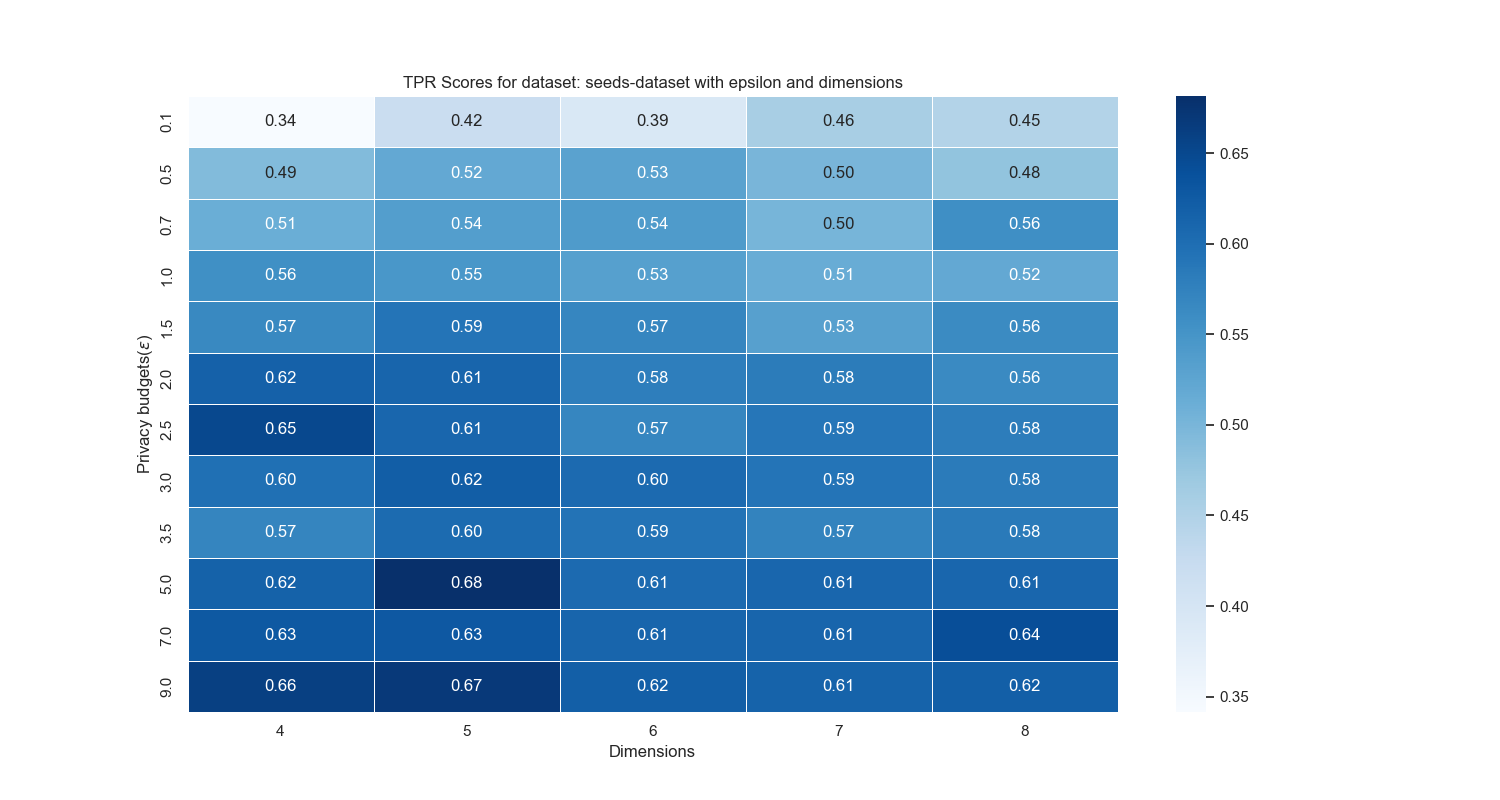
\includegraphics[width=0.8\textwidth]{Results/RQ3/seeds-dataset/security_dimensions_heatmap_nd-laplace-optimal-truncated.png}
    \caption{Heatmap for TPR and dimensionality for the seeds-dataset for kd-Laplace/grid/optimal}
    \label{fig:security_dimensions_heatmap_seeds-dataset_comparison_nd-laplace-optimal-truncated}
    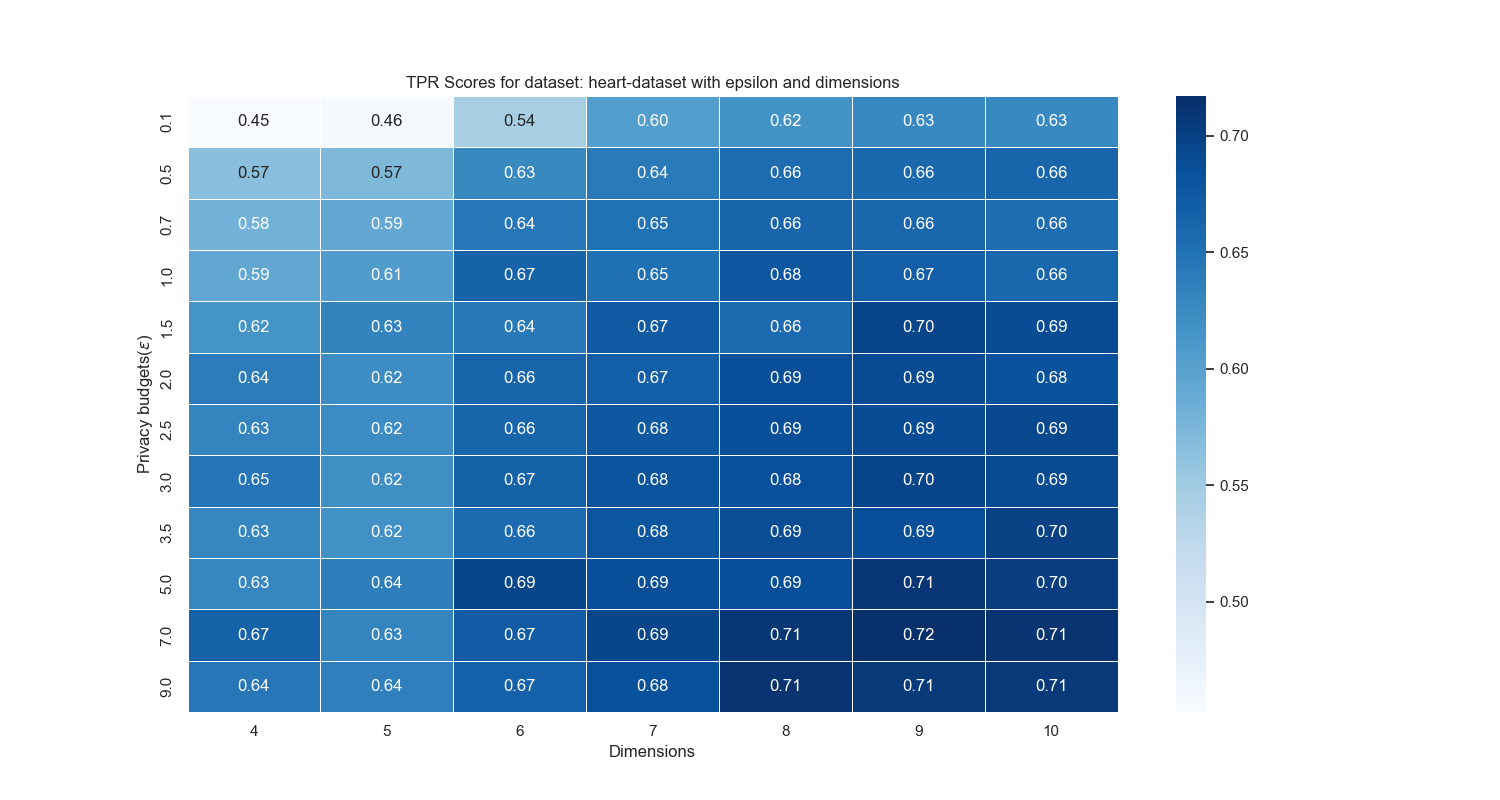
\includegraphics[width=0.8\textwidth]{Results/RQ3/heart-dataset/security_dimensions_heatmap_nd-laplace-optimal-truncated.png}
    \caption{Heatmap for TPR and dimensionality for the heart-dataset for kd-Laplace/grid/optimal}
    \label{fig:security_dimensions_heatmap_hearts-dataset_comparison_nd-laplace-optimal-truncated}
\end{figure}
Generally, a higher epsilon value corresponds to a higher TPR for the seeds dataset. Dimensions 4 and 5 have the highest scores (0.60 >) starting from epsilon 5. The bottom row achieves the highest scores, and for dimensions 4, 5, and 6, TPR values less than 0.40 are reported for epsilon 0.1. No clear trend is visible for the remaining epsilon values based on increasing dimensions.

The heart dataset's lowest scores (< 0.50) are also observed for epsilon 0.1 and dimensions 4 and 5. From epsilon 2 onwards, the values increase (> 0.50 TPR) for dimensions 4 and 5. The heatmap becomes darker for dimensions higher than 5, indicating TPR values higher than 0.60. From epsilon 6 and 8 dimensions, the scores exceed 0.70 TPR.
\newpage

\section{Shape}
\todo[inline]{Uses incorrect k for k-means}
This chapter examines three datasets with a specific shape: circle, line, and left-skewed.
The adversary advantages (privacy) and AMI (utility) are compared between the mechanisms for all three datasets.
We compare kd-Laplace/grid/optimal (green) and Piecewise (yellow).
\begin{figure}[H]
    \begin{minipage}[c]{0.55\textwidth}
        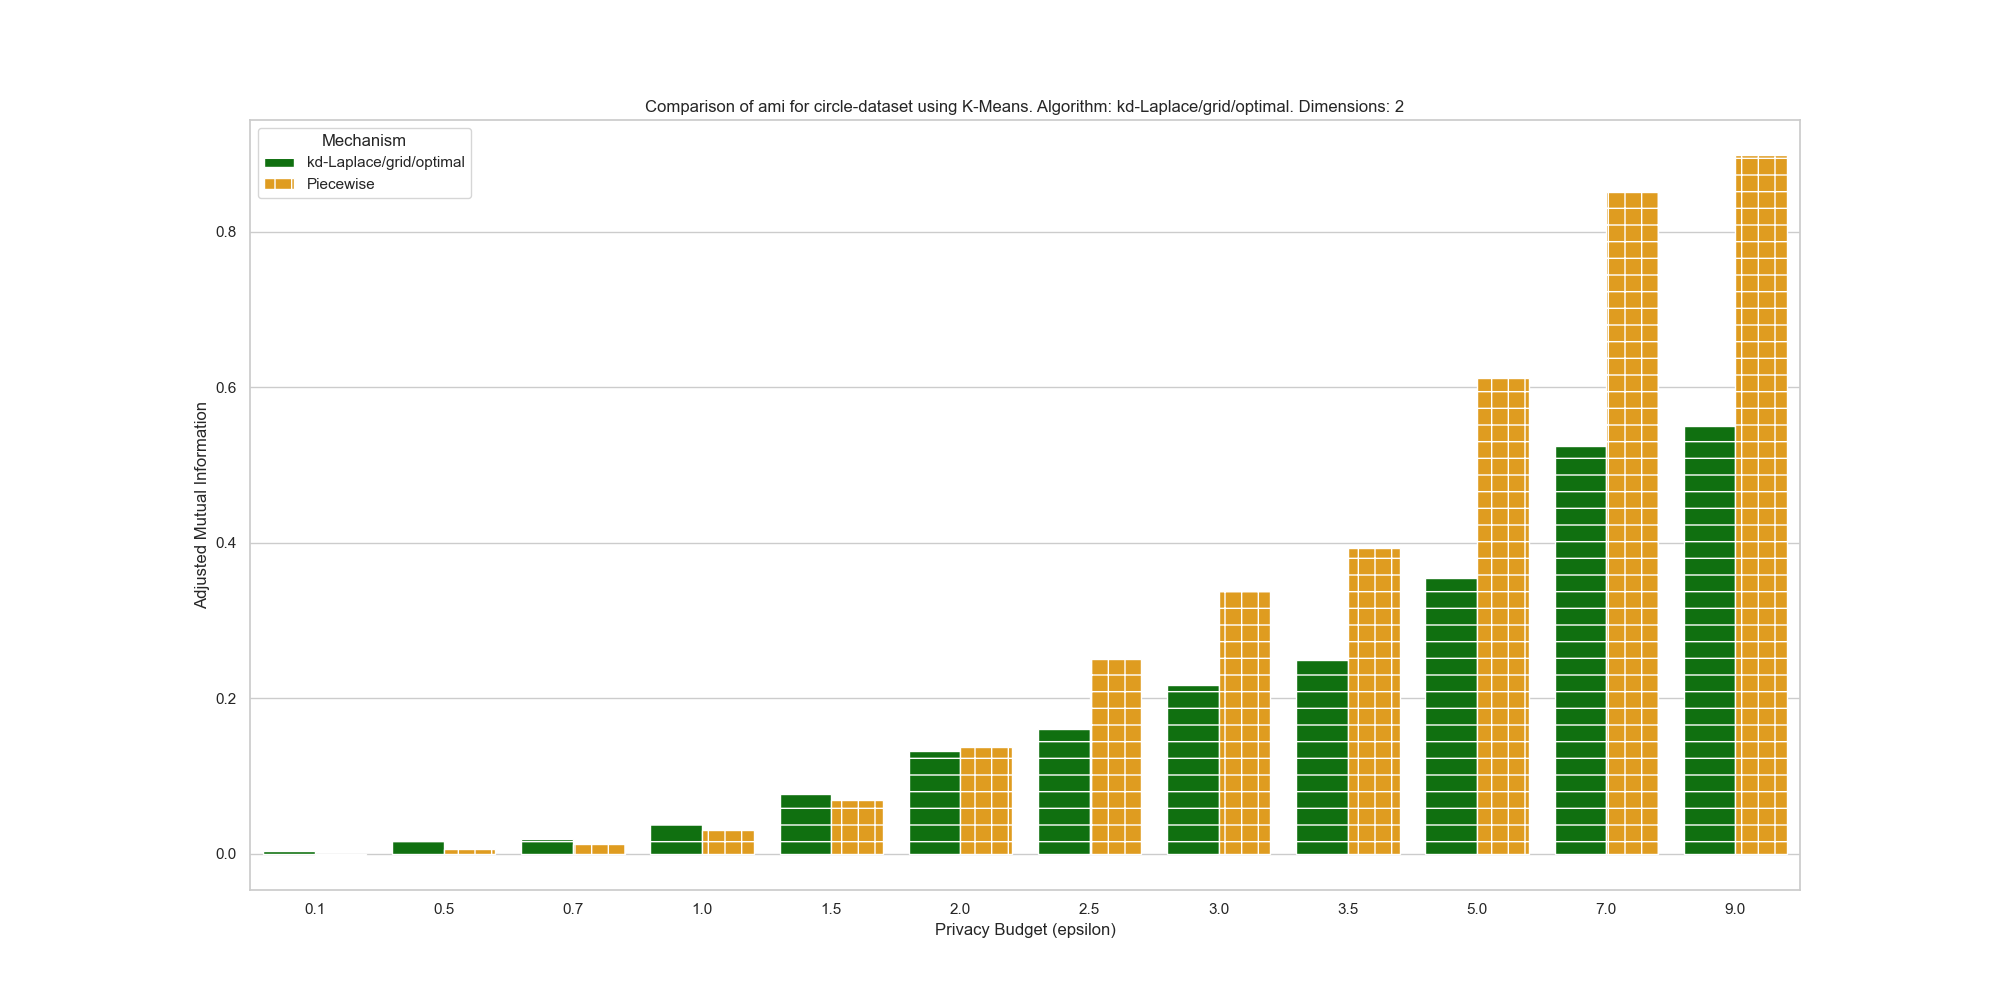
\includegraphics[width=\textwidth]{Results/RQ3/circle-dataset/ami_circle-dataset_comparison.png}
    \end{minipage}
    \begin{minipage}[c]{0.55\textwidth}
        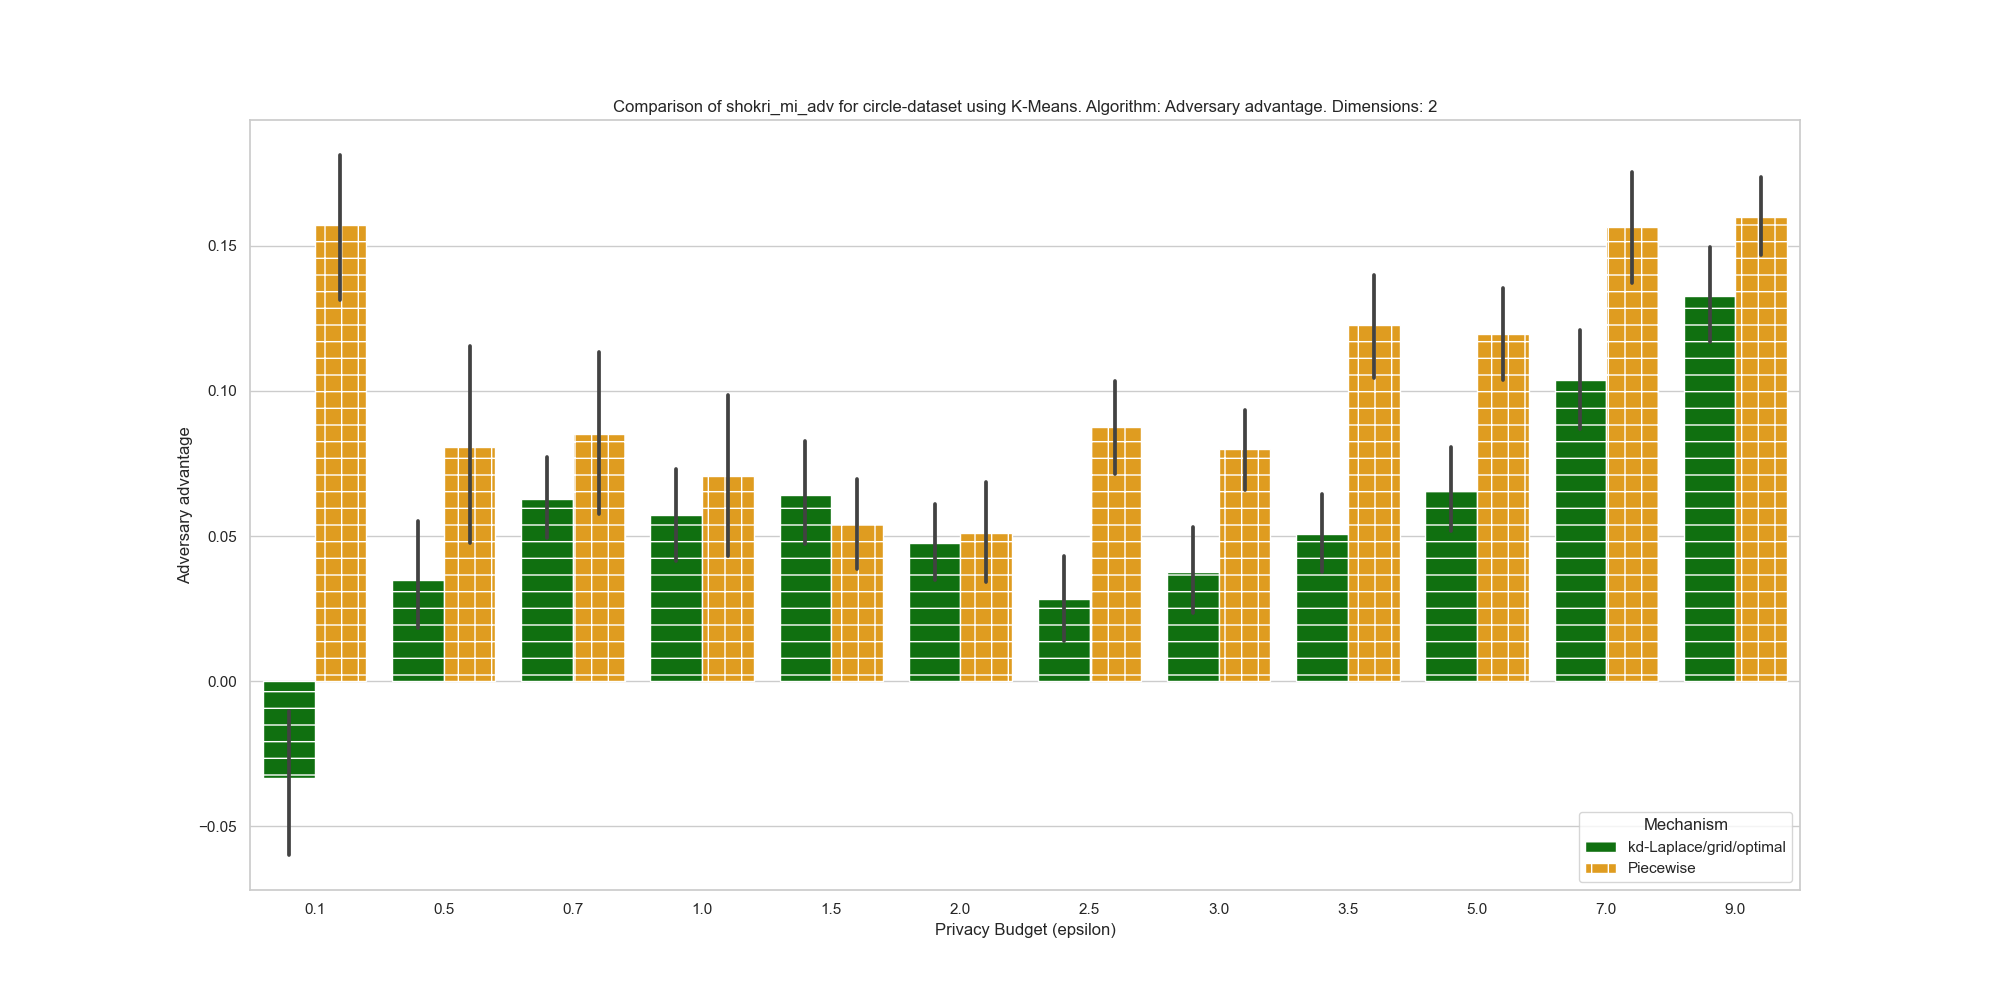
\includegraphics[width=\textwidth]{Results/RQ3/circle-dataset/shokri_mi_adv_circle-dataset_comparison.png}
    \end{minipage}
    \label{fig:advantage_circle-dataset_comparison}
    \caption{The AMI (left) and adversary advantage (right) for the circle-dataset}
\end{figure}
There's a noticeable difference between the Piecewise and kd-Laplace/grid/optimal mechanisms in the circle dataset. For the AMI, Piecewise scores are significantly higher at epsilon 7 to 9. In comparison, kd-Laplace/grid/optimal scores are lower than 0.2 for most other epsilons. Regarding the adversary advantage, kd-Laplace/grid-optimal scores are lower than Piecewise, except for epsilon 1 and 1.5.
\begin{figure}[H]
    \begin{minipage}[c]{0.55\textwidth}
        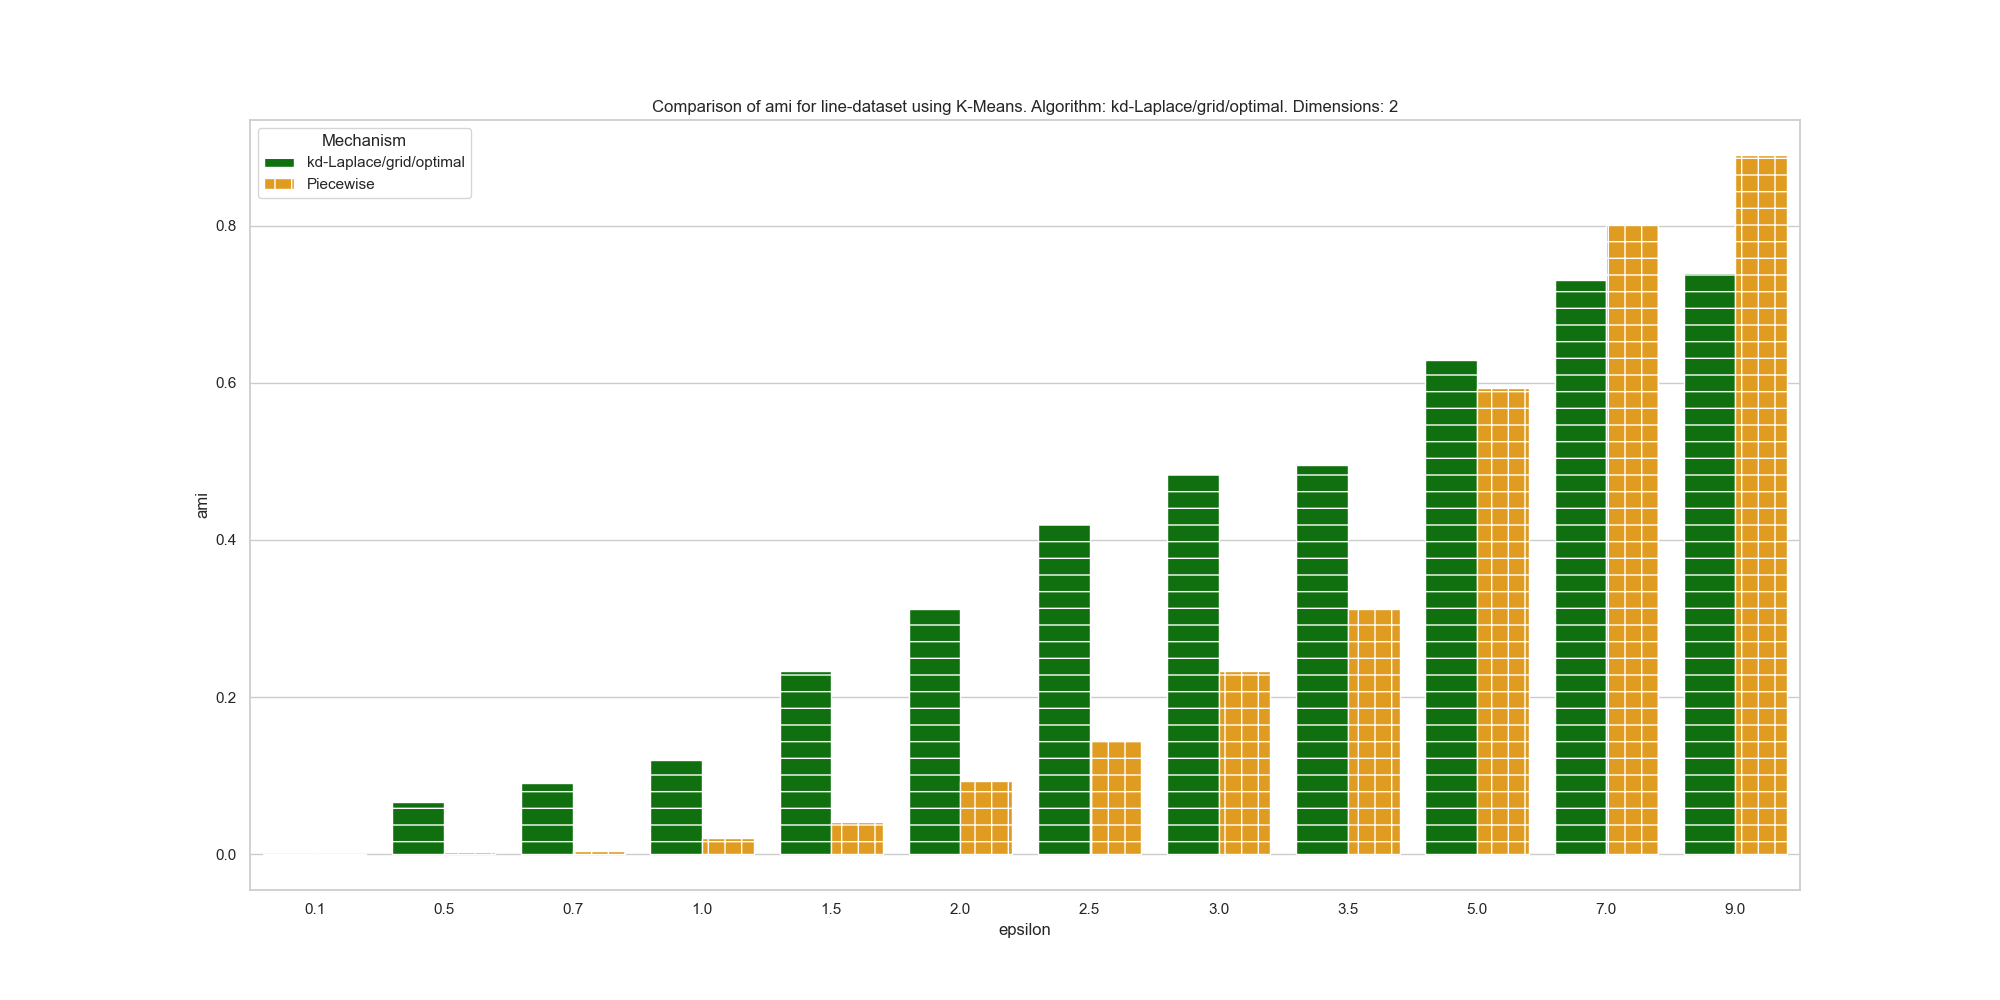
\includegraphics[width=\textwidth]{Results/RQ3/line-dataset/ami_line-dataset_comparison.png}
    \end{minipage}
    \begin{minipage}[c]{0.55\textwidth}
        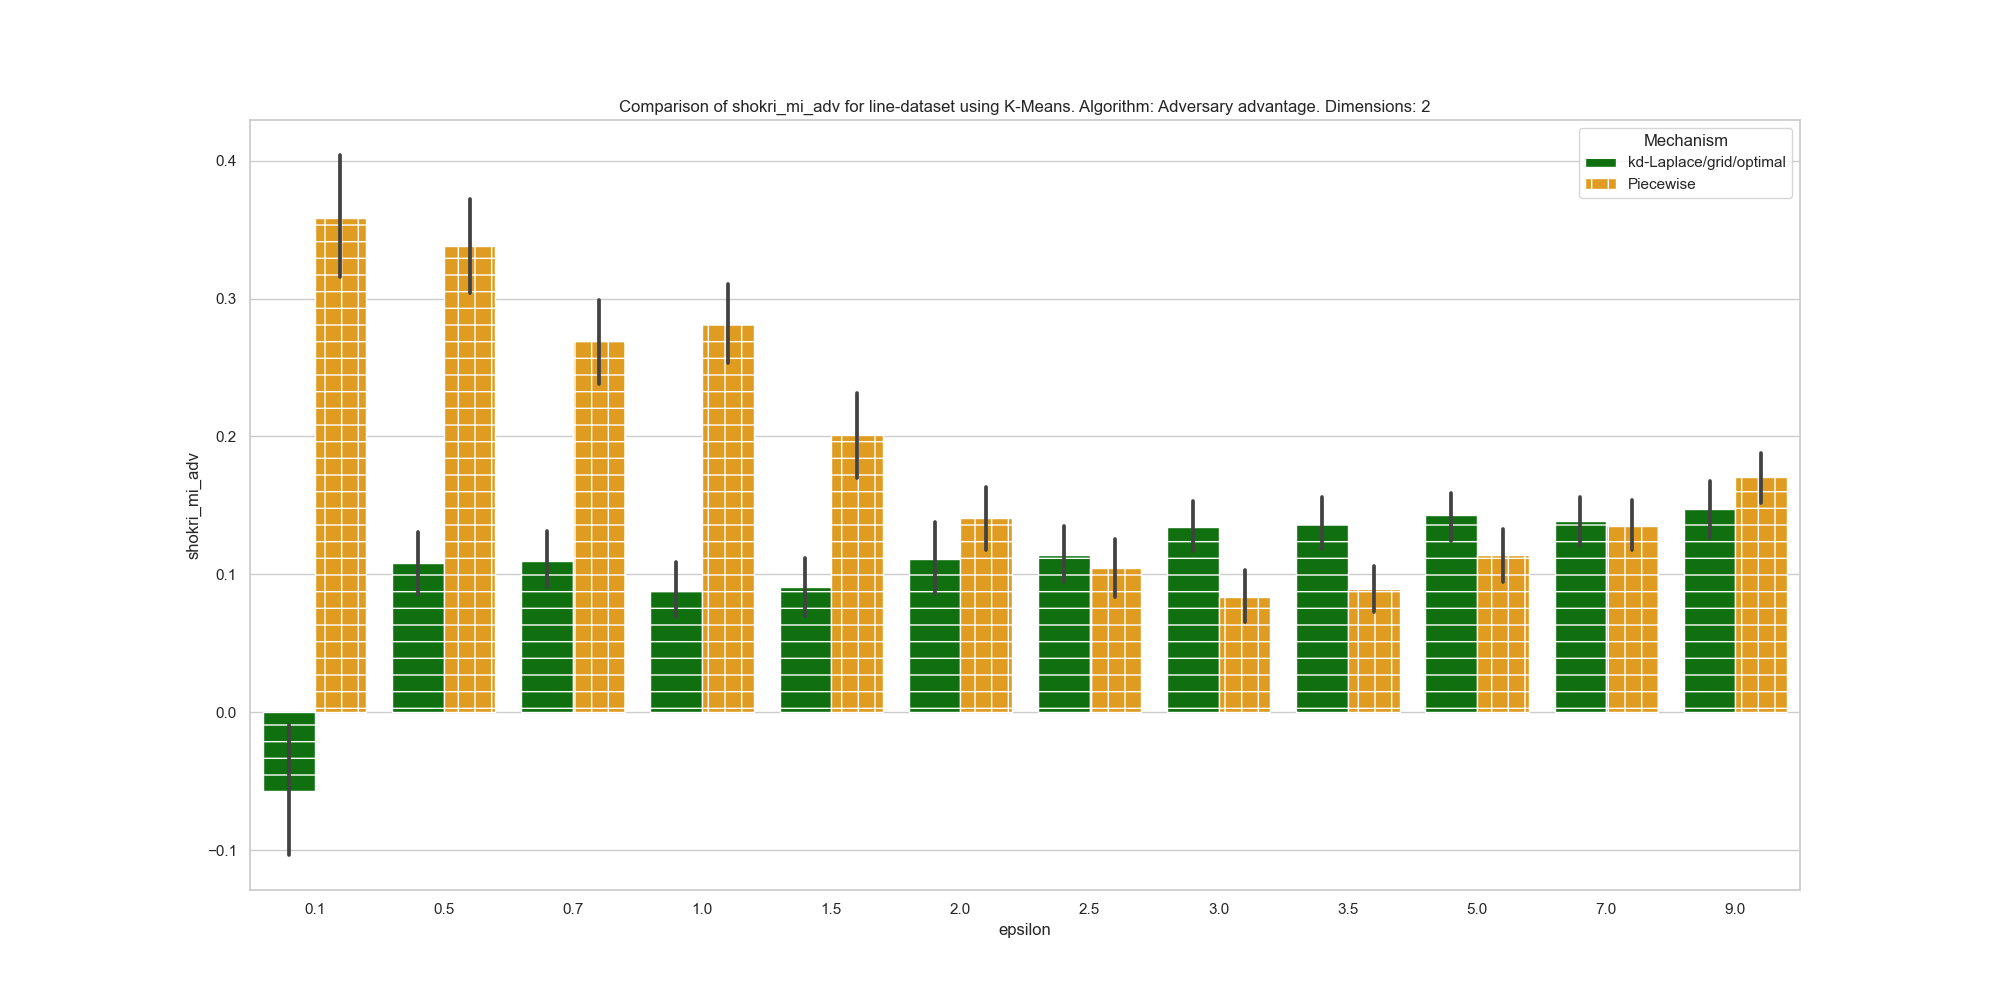
\includegraphics[width=\textwidth]{Results/RQ3/line-dataset/shokri_mi_adv_line-dataset_comparison.png}
    \end{minipage}
    \label{fig:advantage_line-dataset_comparison}
    \caption{The AMI (left) and adversary advantage (right) for the line dataset}
\end{figure}
In the line dataset, Piecewise outperforms kd-Laplace/grid/optimal for epsilon values above 5 for the AMI metric. For epsilons between 0.1 and 5, kd-Laplace/grid/optimal scores are higher. Regarding adversary advantage, Piecewise performs worse for epsilons between 0.1 and 1.5, while kd-Laplace/grid/optimal scores worse for epsilons 2 to 7.
\begin{figure}[H]
    \begin{minipage}[c]{0.55\textwidth}
        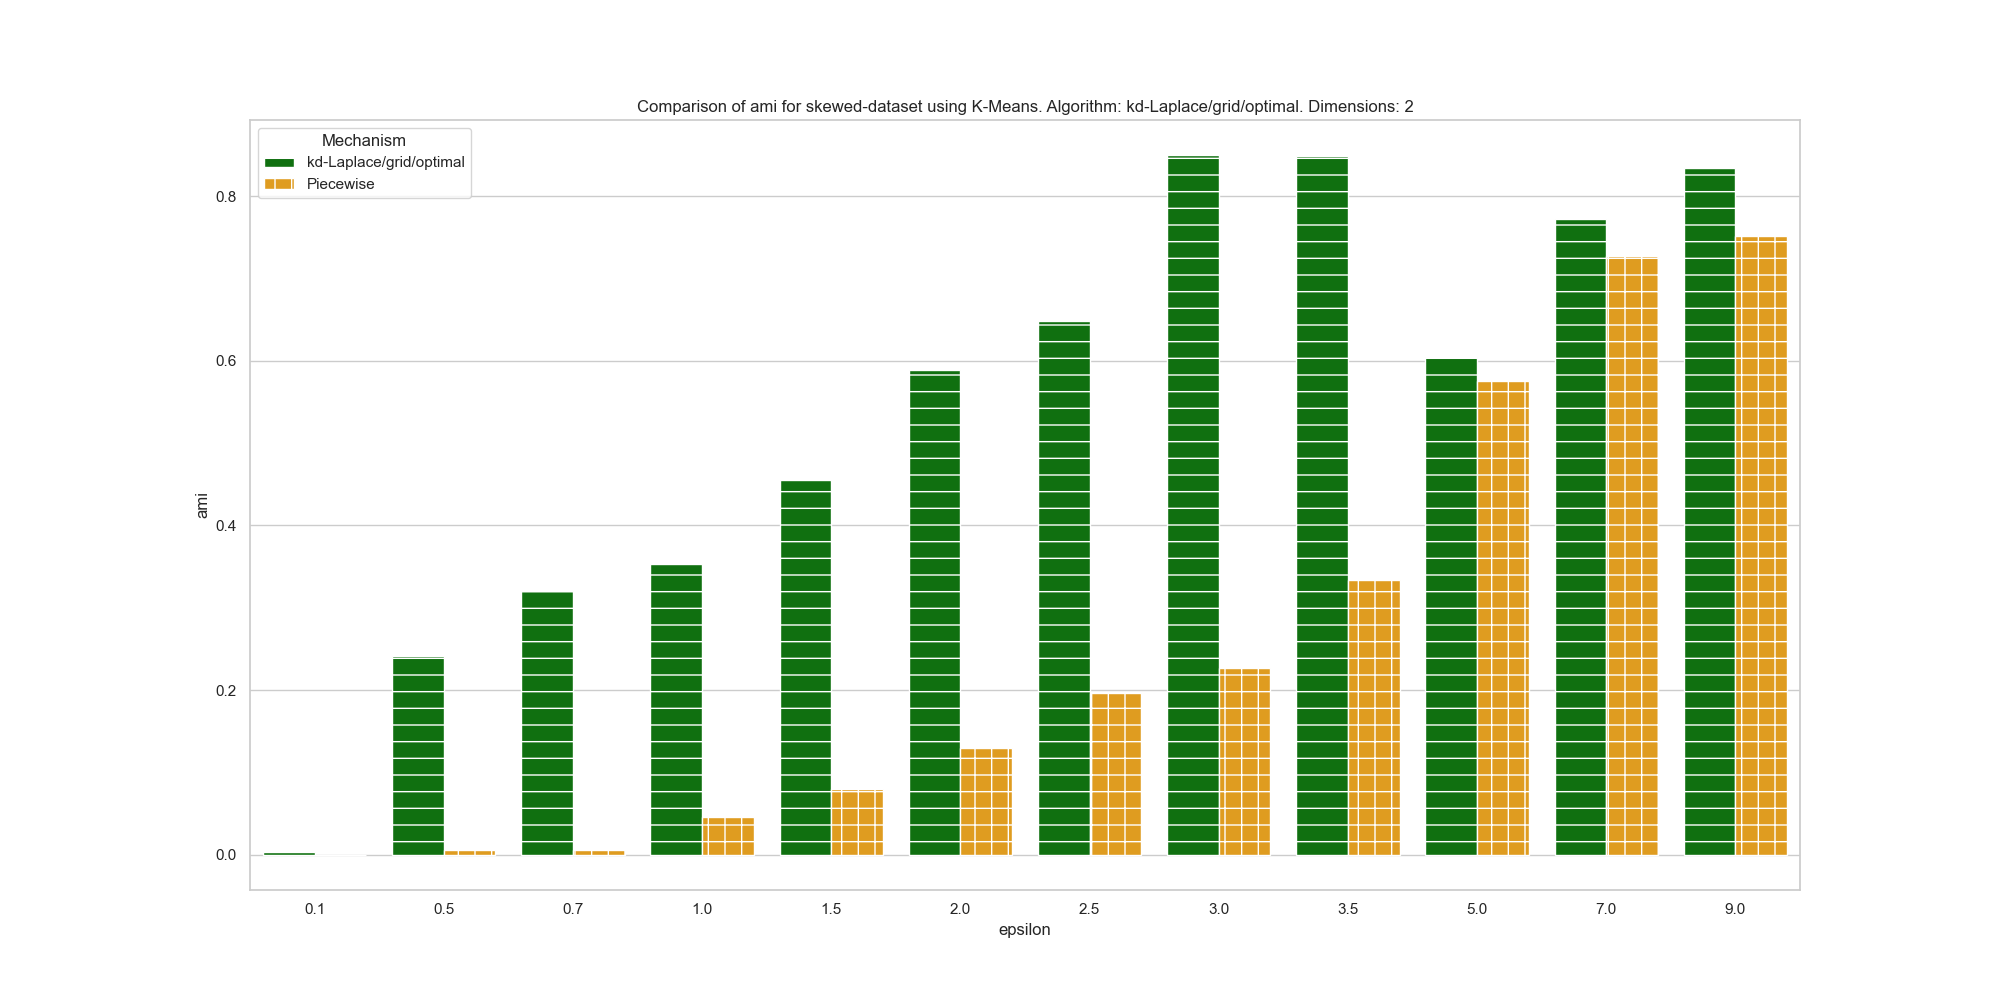
\includegraphics[width=\textwidth]{Results/RQ3/skewed-dataset/ami_skewed-dataset_comparison.png}
    \end{minipage}
    \begin{minipage}[c]{0.55\textwidth}
        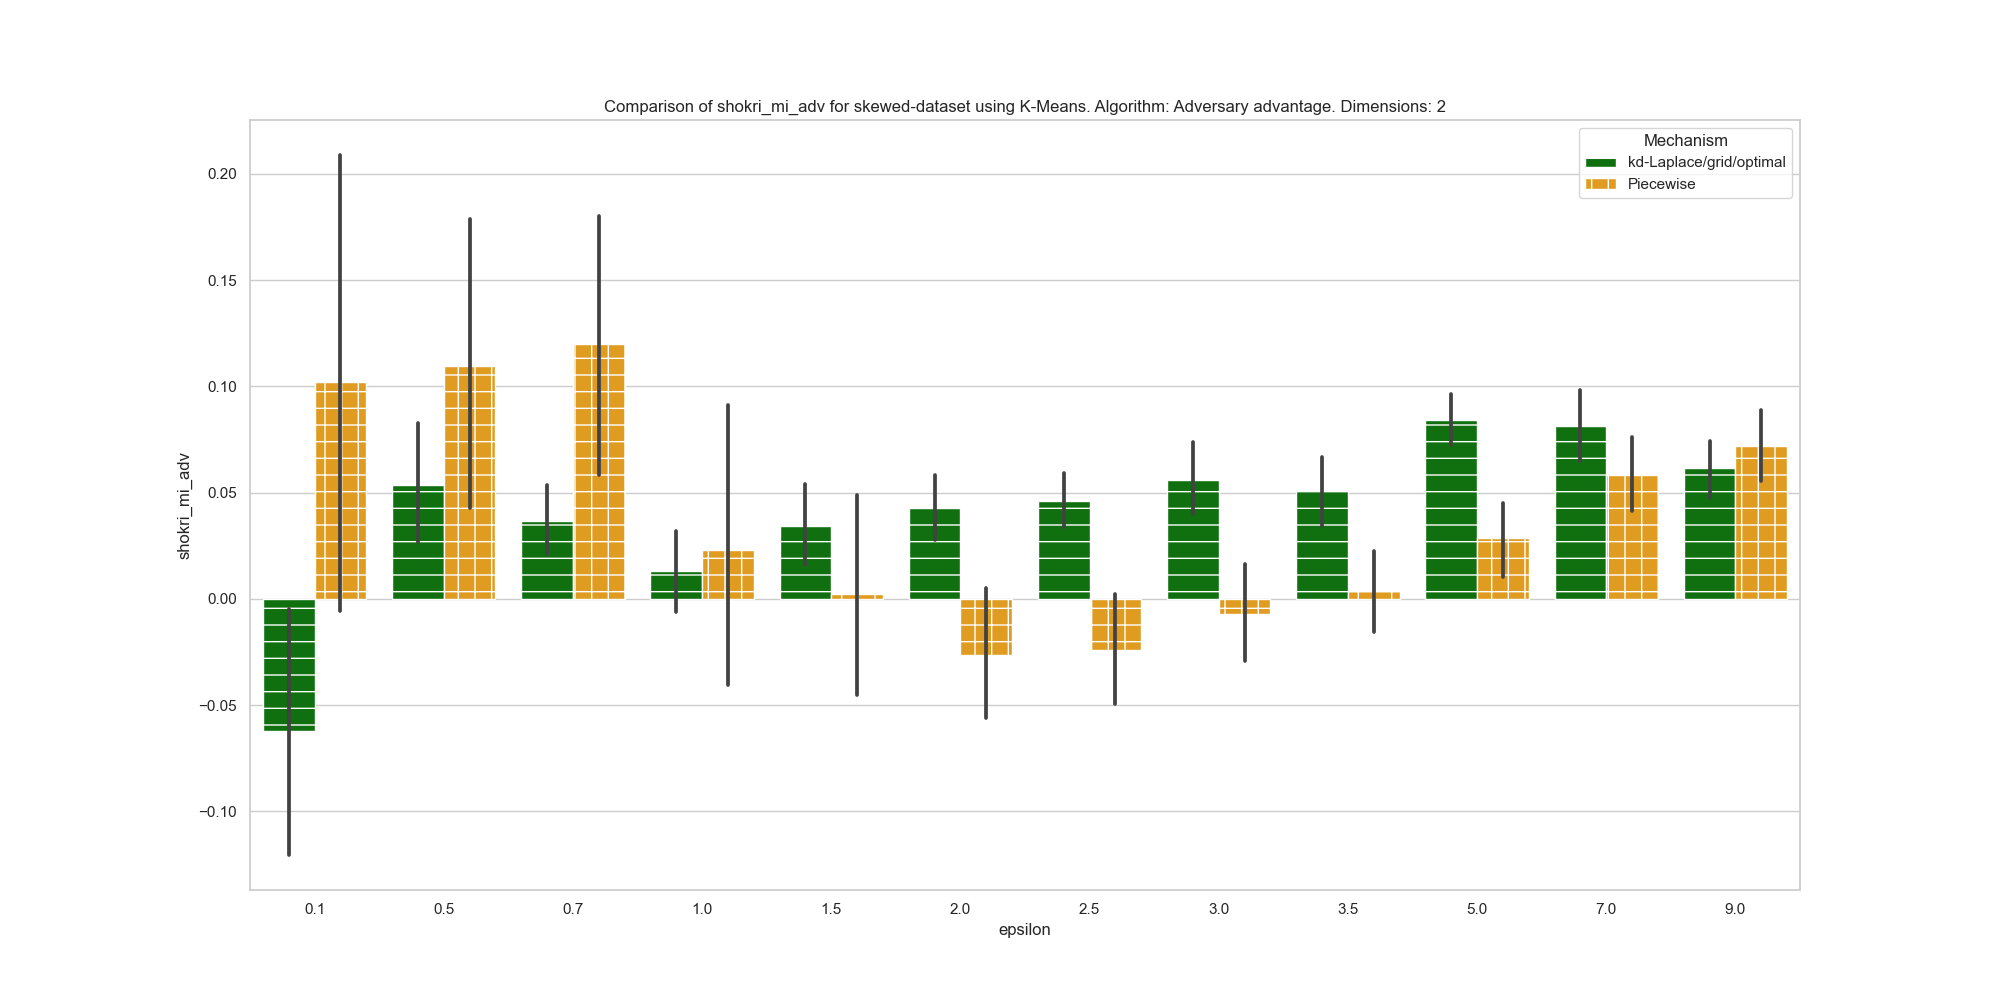
\includegraphics[width=\textwidth]{Results/RQ3/skewed-dataset/shokri_mi_adv_skewed-dataset_comparison.png}
    \end{minipage}
    \label{fig:advantage_skewed-dataset_comparison}
    \caption{The AMI (left) and adversary advantage (right) for the skewed dataset}

\end{figure}
Kd-Laplace/grid/optimal is better than Piecewise for skewed datasets, across all epsilon values, with AMI scores ranging from 0.6 to 0.8. For adversary advantage, Kd-Laplace/grid/optimal outperforms Piecewise between 0.1 and 1.0 epsilon values. The adversary advantage stays low for both mechanisms (below 0.1).


